\documentclass[12pt,a4paper,oneside,openany]{abntex2}
\usepackage[T1]{fontenc}
\usepackage[utf8]{inputenc}
\usepackage[brazil]{babel}
\usepackage{newtxtext,newtxmath}
\usepackage{microtype}
\usepackage{graphicx}
\usepackage{booktabs}
\usepackage{longtable}
\usepackage{tabularx}
\usepackage{array}
\usepackage{float}
\usepackage{caption}
\usepackage{setspace}
\usepackage{indentfirst}
\usepackage{hyperref}
\usepackage{enumitem}
\usepackage{geometry}
\usepackage{needspace}
\usepackage{xurl}
\urlstyle{same}
\usepackage[section]{placeins}
\raggedbottom
\clubpenalty=10000
\widowpenalty=10000
\displaywidowpenalty=10000
\setcounter{topnumber}{3}
\renewcommand{\topfraction}{0.9}
\renewcommand{\textfraction}{0.1}
\renewcommand{\floatpagefraction}{0.7}
\geometry{top=3cm,left=3cm,right=2cm,bottom=2cm}
\setlength{\parindent}{1.25cm}
\setlength{\parskip}{0pt}
\OnehalfSpacing
\counterwithout{table}{chapter}
\captionsetup{font={footnotesize,singlespacing},labelfont=normal,justification=centering,labelsep=endash,skip=3pt}
\addto\captionsbrazil{%
\renewcommand{\listfigurename}{LISTA DE FIGURAS}%
\renewcommand{\tablename}{Quadro}%
\renewcommand{\listtablename}{LISTA DE QUADROS}%
\renewcommand{\contentsname}{SUMÁRIO}%
\renewcommand{\resumoname}{RESUMO}%
\renewcommand{\agradecimentosname}{AGRADECIMENTOS}%
\renewcommand{\listadesiglasname}{LISTA DE ABREVIATURAS E SIGLAS}%
}
\makepagestyle{tcc}
\makeevenhead{tcc}{}{}{\thepage}
\makeoddhead{tcc}{}{}{\thepage}
\makeevenfoot{tcc}{}{}{}
\makeoddfoot{tcc}{}{}{}
\hypersetup{hidelinks,pdfauthor={Eduardo Henrique Guimarães Marques},pdftitle={Desenvolvimento de Plataforma Web para Apoio à Análise de EEG com Inteligência Artificial Explicável}}

\makeatletter
\renewcommand{\ABNTEXchapterfont}{\bfseries}
\renewcommand{\ABNTEXchapterfontsize}{\normalsize}
\renewcommand{\ABNTEXsectionfont}{\normalfont}
\renewcommand{\ABNTEXsectionfontsize}{\normalsize}
\renewcommand{\ABNTEXsubsectionfont}{\normalfont}
\renewcommand{\ABNTEXsubsectionfontsize}{\normalsize}
\setlength{\beforechapskip}{0pt}
\setlength{\midchapskip}{0pt}
\setlength{\afterchapskip}{9pt}
\setbeforesecskip{0pt}
\setaftersecskip{5pt}
\setbeforesubsecskip{0pt}
\setaftersubsecskip{5pt}
\makeatother

\begin{document}
\selectlanguage{brazil}
\frenchspacing
\pretextual
\begin{capa}
{\linespread{1.15}\selectfont
\begin{center}
INSTITUTO FEDERAL DE EDUCAÇÃO, CIÊNCIA E TECNOLOGIA DE GOIÁS -- CÂMPUS URUAÇU\par
DEPARTAMENTO DE ÁREAS ACADÊMICAS\par
CURSO DE TECNOLOGIA EM ANÁLISE E DESENVOLVIMENTO DE SISTEMAS\par
\vspace*{110pt}
EDUARDO HENRIQUE GUIMARÃES MARQUES\par
\vspace*{130pt}
\textbf{DESENVOLVIMENTO DE PLATAFORMA WEB PARA APOIO À ANÁLISE DE EEG COM INTELIGÊNCIA ARTIFICIAL EXPLICÁVEL}\par
\vfill
URUAÇU/GO\par
2026\par
\end{center}
}
\end{capa}

\begin{folhaderosto}
{\linespread{1.15}\selectfont
\begin{center}
EDUARDO HENRIQUE GUIMARÃES MARQUES\par
\vspace*{120pt}
\textbf{DESENVOLVIMENTO DE PLATAFORMA WEB PARA APOIO À ANÁLISE DE EEG COM INTELIGÊNCIA ARTIFICIAL EXPLICÁVEL}\par
\vspace*{90pt}
\hspace*{8.5cm}\begin{minipage}{7.2cm}
\fontsize{10}{12}\selectfont
\begin{SingleSpace}
Trabalho de Conclusão de Curso apresentado ao curso de Tecnologia em Análise e Desenvolvimento de Sistemas do Departamento de Áreas Acadêmicas do Instituto Federal de Educação, Ciência e Tecnologia de Goiás -- Câmpus Uruaçu como requisito parcial para conclusão do curso.

\vspace{0.8cm}
Orientador: Dr. Lynwood Livi de Souza
\end{SingleSpace}
\end{minipage}
\par\vfill
URUAÇU/GO\par
2026\par
\end{center}
}
\end{folhaderosto}

\begin{agradecimentos}
Agradeço primeiramente a Deus, pela saúde, força e perseverança concedidas ao longo de toda a minha caminhada acadêmica.

Aos meus pais e à minha família, pelo apoio incondicional, compreensão e incentivo constante em cada etapa da minha formação.

Ao meu orientador, Prof. Dr. Lynwood Livi de Souza, pela orientação criteriosa, paciência, disponibilidade e pelas valiosas contribuições técnicas e científicas que guiaram a evolução deste trabalho desde a iniciação tecnológica até a conclusão deste curso.

Ao Instituto Federal de Educação, Ciência e Tecnologia de Goiás (IFG) – Câmpus Uruaçu, e a todos os professores do Curso de Tecnologia em Análise e Desenvolvimento de Sistemas, pelos ensinamentos transmitidos e pela dedicação à educação pública e de qualidade.

Aos colegas de curso e amigos que compartilharam desafios, aprendizados e momentos importantes durante a graduação, e aos membros da banca examinadora, pela disponibilidade e pelas contribuições para o aperfeiçoamento deste trabalho.
\end{agradecimentos}

\begin{resumo}
A interpretação de exames de Eletroencefalograma (EEG) no diagnóstico da epilepsia exige a inspeção visual de longas séries temporais multicanais, processo sujeito à fadiga e à variabilidade entre avaliadores. Embora modelos de aprendizado profundo possam reconhecer padrões complexos, sua aplicação clínica enfrenta a fragmentação entre ferramentas e a dificuldade de inspecionar as decisões das redes neurais. Este trabalho desenvolveu e avaliou o protótipo funcional de uma plataforma web integrada (EEG-XAI) voltada ao apoio à triagem e à análise neurofisiológica. A solução adota arquitetura cliente-servidor mediada por API REST e combina uma interface em React, TypeScript e Recharts com um núcleo de processamento em Python, FastAPI, MNE-Python, TensorFlow/Keras e PostgreSQL. No motor preditivo, implementou-se a arquitetura híbrida CNN-BiLSTM v43, com fusão tardia de 23 canais e sequências de 15 características tempo-frequência por canal, incluindo entropia espectral. Para aumentar a inspecionabilidade, o Gradient SHAP foi integrado ao pipeline e suas relevâncias positivas foram projetadas sobre o traçado, por canal e intervalo temporal, para a sequência de pico. Nos experimentos com registros contínuos da base pública CHB-MIT, os grupos de treino e calibração foram separados antes do janelamento. Na calibração, o modelo atingiu F1 por EDF de 95,7\%, F1 localizado de 90,9\% e detecção de 15 em 20 eventos ictais, com 0,55 falso alarme por hora. Na avaliação histórica de desenvolvimento, obteve F1 por EDF de 82,4\%, F1 localizado de 46,2\% e detecção de 4 em 9 eventos, evidenciando a dificuldade de generalização interpaciente. Conclui-se que a plataforma integra ingestão de EDF, navegação multicanal, localização temporal de trechos suspeitos, explicabilidade visual e emissão de laudos, oferecendo apoio computacional à revisão médica sem substituir o diagnóstico clínico.

\vspace{\onelineskip}
\noindent\textbf{Palavras-chave}: eletroencefalograma; epilepsia; aprendizado profundo; CNN-BiLSTM; inteligência artificial explicável; SHAP.
\end{resumo}

\begin{resumo}[ABSTRACT]
\begin{otherlanguage*}{english}
Interpreting Electroencephalogram (EEG) exams for epilepsy diagnosis requires visual inspection of long multichannel time series, a process subject to fatigue and inter-observer variability. Although deep learning models can recognize complex patterns, their clinical application faces fragmented workflows and limited decision inspectability. This work developed and evaluated a functional integrated web platform prototype (EEG-XAI) to support neurophysiological triage and analysis. The solution adopts a REST API-mediated client-server architecture and combines a React, TypeScript, and Recharts interface with a processing core based on Python, FastAPI, MNE-Python, TensorFlow/Keras, and PostgreSQL. Its predictive engine implements the v43 hybrid CNN-BiLSTM architecture with late fusion across 23 channels and sequences of 15 time-frequency features per channel, including spectral entropy. To increase inspectability, Gradient SHAP was integrated into the pipeline, and positive relevance values for the peak sequence were projected onto the trace by channel and time interval. In experiments with continuous recordings from the public CHB-MIT dataset, training and calibration groups were separated before windowing. In calibration, the model achieved an EDF-level F1-score of 95.7\%, a localized F1-score of 90.9\%, and detected 15 of 20 ictal events, with 0.55 false alarms per hour. In the historical development evaluation, it achieved an EDF-level F1-score of 82.4\%, a localized F1-score of 46.2\%, and detected 4 of 9 events, highlighting the difficulty of inter-patient generalization. The platform integrates EDF ingestion, multichannel navigation, temporal localization of suspicious segments, visual explainability, and medical reporting, providing computational support for specialist review without replacing clinical diagnosis.

\vspace{\onelineskip}
\noindent\textbf{Keywords}: electroencephalogram; epilepsy; deep learning; CNN-BiLSTM; explainable artificial intelligence; SHAP.
\end{otherlanguage*}
\end{resumo}

\pdfbookmark[0]{\listfigurename}{lof}
\listoffigures*
\cleardoublepage
\pdfbookmark[0]{LISTA DE QUADROS}{loq}
\listoftables*
\cleardoublepage

\begin{siglas}
\item[ANVISA] Agência Nacional de Vigilância Sanitária
\item[API] Application Programming Interface (Interface de Programação de Aplicações)
\item[BiLSTM] Bidirectional Long Short-Term Memory (Memória de Longo e Curto Prazo Bidirecional)
\item[CDSS] Clinical Decision Support Systems (Sistemas de Suporte à Decisão Clínica)
\item[CHB-MIT] Children's Hospital Boston - Massachusetts Institute of Technology
\item[CNN] Convolutional Neural Network (Rede Neural Convolucional)
\item[CPF] Cadastro de Pessoas Físicas
\item[CRM] Conselho Regional de Medicina
\item[EDF] European Data Format
\item[EEG] Eletroencefalograma
\item[eMAG] Modelo de Acessibilidade em Governo Eletrônico
\item[FROC] Free-Response Receiver Operating Characteristic
\item[HTTP] Hypertext Transfer Protocol
\item[IA] Inteligência Artificial
\item[IFG] Instituto Federal de Educação, Ciência e Tecnologia de Goiás
\item[I/O] Input/Output (Entrada/Saída)
\item[IoU] Intersection over Union (Interseção sobre União)
\item[JSON] JavaScript Object Notation
\item[JWT] JSON Web Token
\item[LGPD] Lei Geral de Proteção de Dados Pessoais
\item[LSTM] Long Short-Term Memory (Memória de Longo e Curto Prazo)
\item[MER] Modelo Entidade-Relacionamento
\item[MLP] Multi-Layer Perceptron (Perceptron Multicamadas)
\item[P\&D] Pesquisa e Desenvolvimento
\item[PIBITI] Programa Institucional de Bolsas de Iniciação em Desenvolvimento Tecnológico e Inovação
\item[RDC] Resolução da Diretoria Colegiada
\item[REST] Representational State Transfer
\item[RF] Requisito Funcional
\item[RNF] Requisito Não Funcional
\item[SADC] Sistema de Apoio à Decisão Clínica
\item[SHAP] Shapley Additive exPlanations
\item[SOA] Service-Oriented Architecture (Arquitetura Orientada a Serviços)
\item[SPA] Single Page Application
\item[UI] User Interface (Interface de Usuário)
\item[WCAG] Web Content Accessibility Guidelines
\item[WHO] World Health Organization (Organização Mundial da Saúde)
\item[XAI] Explainable Artificial Intelligence (Inteligência Artificial Explicável)
\end{siglas}

\pdfbookmark[0]{\contentsname}{toc}
\tableofcontents*
\cleardoublepage

\cleardoublepage
\textual
\pagestyle{tcc}\aliaspagestyle{chapter}{tcc}
\chapter{INTRODUÇÃO}
O Eletroencefalograma (EEG) constitui uma ferramenta fundamental para o diagnóstico e o monitoramento da epilepsia, pois registra com elevada resolução temporal a atividade elétrica cerebral. A análise de registros extensos, contudo, permanece predominantemente visual, demanda tempo especializado e está sujeita à fadiga e à variabilidade entre avaliadores (Tatum, 2014; Roy et al., 2019). Esse cenário reforça a necessidade de ferramentas computacionais capazes de apoiar a triagem sem substituir a decisão médica.

Embora técnicas de Deep Learning apresentem potencial para reconhecer padrões complexos em EEG, sua incorporação ao fluxo clínico enfrenta barreiras técnicas e operacionais. Entre elas estão a fragmentação entre ferramentas de armazenamento e visualização, a dependência de soluções proprietárias, a dificuldade de processar exames multicanais extensos e a opacidade das redes neurais profundas. Um classificador isolado não resolve integralmente o problema: o especialista também precisa importar o exame, navegar pelos canais, localizar os eventos suspeitos, avaliar a explicação do modelo e registrar seu próprio parecer.

Diante dessa lacuna, o presente trabalho desenvolveu um protótipo funcional de plataforma web para apoio à triagem e à análise de EEG. A solução centraliza a ingestão de arquivos EDF, a visualização multicanal, a inferência temporal por uma rede CNN-BiLSTM e a apresentação de trechos suspeitos. A arquitetura cliente-servidor mediada por API REST separa a interface do núcleo de processamento e permite evoluir cada componente de forma independente.

A explicabilidade é incorporada por meio do método SHAP, que relaciona a decisão da rede às características, aos canais e aos intervalos temporais analisados. O sistema deve ser compreendido como ferramenta experimental de segunda opinião, com potencial para apoiar a produtividade e direcionar a revisão do especialista, e não como substituto do diagnóstico clínico. Por lidar com informações de saúde, sua evolução também deve considerar acessibilidade, privacidade, segurança e o enquadramento regulatório aplicável a Software como Dispositivo Médico.

No Brasil, a eventual disponibilização de software com finalidade médica deve considerar a regulamentação aplicável a Software como Dispositivo Médico, incluindo a RDC nº 657, de 24 de março de 2022, da Agência Nacional de Vigilância Sanitária. O protótipo desenvolvido neste trabalho não foi submetido à regularização sanitária. No âmbito da interface, as recomendações do eMAG e das WCAG constituem referências para evolução da acessibilidade, sem que se alegue conformidade formal antes de uma auditoria específica.

Em termos operacionais, a pergunta central é: como reunir, em uma aplicação web, a inspeção de um EEG extenso e a indicação automática de intervalos que merecem revisão? O resultado entregue combina duas contribuições: um fluxo funcional de software e uma avaliação quantitativa do detector temporal. O médico recebe o traçado, os intervalos suspeitos e as contribuições estimadas pelo modelo, podendo confrontá-los antes de registrar seu parecer. O desempenho do detector é avaliado separadamente do funcionamento da aplicação.

\Needspace{12\baselineskip}\section{OBJETIVOS}
\subsection{Objetivo Geral}
Desenvolver e avaliar um protótipo funcional de plataforma web para apoio à triagem e à análise de exames de Eletroencefalograma (EEG), integrando uma arquitetura híbrida CNN-BiLSTM e técnicas de Inteligência Artificial Explicável (XAI) para localizar temporalmente eventos suspeitos e fornecer informações de apoio à revisão do especialista.

\subsection{Objetivos Específicos}
Os objetivos específicos a seguir foram definidos para viabilizar o alcance do objetivo geral:

\begin{itemize}[leftmargin=1.25cm,itemsep=0pt,topsep=0pt]
\item Levantar e documentar requisitos funcionais e não funcionais relacionados à ingestão, ao processamento, à visualização, à segurança e à interpretabilidade de sinais de EEG.
\item Implementar uma interface web responsiva, desenvolvida em React, para importação de EDF, navegação temporal, zoom e seleção dinâmica de canais.
\item Desenvolver um módulo de ingestão capaz de validar arquivos EDF, extrair seus metadados e preservar a identidade dos canais durante a análise.
\item Estruturar o janelamento temporal depois da separação dos pacientes entre treino e calibração, ampliando a quantidade de exemplos sem provocar vazamento de dados.
\item Investigar Entropia de Shannon e Dinâmica Simbólica como características candidatas e selecionar, por avaliação experimental, a representação de entrada da CNN-BiLSTM temporal.
\item Integrar o método SHAP para representar a relevância das características por canal e por intervalo temporal sobre o traçado do EEG.
\item Avaliar o modelo em registros públicos da CHB-MIT por EDF, evento e localização temporal, utilizando precisão, sensibilidade, F1, IoU e falsos alarmes por hora.
\end{itemize}
\Needspace{12\baselineskip}\section{Justificativa}
A leitura manual de EEG é extensa e depende de conhecimento especializado, enquanto classificadores isolados não oferecem necessariamente o fluxo de ingestão, visualização, explicação e registro do parecer. O projeto busca enfrentar essa lacuna por meio de uma plataforma integrada, preservando a supervisão humana e apresentando a saída da IA como trecho suspeito, e não como diagnóstico final.

A proposta fundamenta-se na experiência adquirida no projeto de iniciação tecnológica Identificação de Padrões Genéticos para Diagnóstico de Doenças Utilizando Inteligência Artificial, posteriormente direcionado à análise de sinais bioelétricos (Moreira et al., 2025). O trabalho anterior demonstrou a viabilidade de extrair características matemáticas de séries temporais; o presente projeto amplia essa contribuição ao incorporar tais técnicas a um fluxo web completo.

A disponibilização por navegador reduz a dependência de instalações proprietárias em cada estação de trabalho e permite centralizar o processamento computacional no servidor. Essa estratégia não elimina custos de infraestrutura, mas favorece manutenção, atualização e acesso controlado. A integração entre visualização, modelo temporal e XAI também contribui para que a predição seja inspecionada no contexto do sinal original.

A relevância acadêmica decorre da aplicação conjunta de Engenharia de Software, processamento de sinais, aprendizado profundo e interpretabilidade. O resultado esperado é um protótipo verificável, acompanhado de métricas e limitações explícitas, que possa servir de base para estudos posteriores de generalização interpaciente, usabilidade e validação com especialistas.

\Needspace{12\baselineskip}\section{Organização do Trabalho}
Este trabalho encontra-se estruturado em sete capítulos. O Capítulo 1 introduz o contexto clínico e computacional da análise de EEG, definindo os objetivos geral e específicos, bem como a justificativa da pesquisa. O Capítulo 2 apresenta o referencial teórico, abordando os fundamentos neurofisiológicos, a engenharia de software orientada a serviços, a persistência de dados biomédicos, as arquiteturas híbridas de aprendizado profundo com explicabilidade (XAI) e a transformação digital no apoio diagnóstico. O Capítulo 3 descreve a metodologia adotada, detalhando o levantamento de requisitos, as tecnologias utilizadas, os incrementos de desenvolvimento, os protocolos de teste e a implementação. O Capítulo 4 documenta a engenharia do software, contemplando os requisitos funcionais e não funcionais, os casos de uso, a arquitetura cliente-servidor, o fluxograma operacional, o modelo de dados e os protótipos de baixa fidelidade. O Capítulo 5 apresenta os resultados alcançados, englobando a interface real implementada, o protocolo experimental na base CHB-MIT, o desempenho do modelo v43, a análise de estabilidade entre seeds e a verificação dos artefatos. O Capítulo 6 discute as implicações dos achados, as limitações técnicas e as ameaças à validade do estudo. Por fim, o Capítulo 7 sintetiza as conclusões do trabalho e aponta direções para pesquisas futuras.

\chapter{REFERENCIAL TEÓRICO}
\Needspace{12\baselineskip}\section{Contexto Neurofisiológico e Desafios da Análise Computacional}
O Eletroencefalograma (EEG) é reconhecido como recurso fundamental para o diagnóstico e o monitoramento de epilepsia e outras desordens cerebrais, caracterizando-se como exame não invasivo, de baixo custo e elevada resolução temporal (Niedermeyer; Lopes da Silva, 2005; Craik et al., 2019). A duração dos registros e a quantidade de canais produzem grande volume de dados, o que aumenta a carga de revisão dos especialistas.

Apesar da importância do exame, a interpretação do EEG ainda é predominantemente manual e visual. Relatórios e estudos da área indicam que a análise de longas séries temporais (exames que podem durar de 20 minutos a dias) é um processo exaustivo, sujeito à fadiga e à subjetividade do especialista (Tatum, 2014; Roy et al., 2019). A leitura visual convencional pode ser lenta, apresentar variabilidade entre avaliadores e dificultar a detecção de eventos sutis ou raros em meio a artefatos (Aboalayon et al., 2016).

Diante da complexidade não linear dos sinais biológicos, a Inteligência Artificial passou a ser investigada como recurso de apoio à decisão clínica (Topol, 2019). Nesse contexto, sistemas de apoio à decisão (CDSS - Clinical Decision Support Systems) podem contribuir para a triagem em larga escala, desde que seu desempenho e seus riscos sejam avaliados no cenário de uso (Sutton et al., 2020). A adoção de algoritmos de Deep Learning pode auxiliar a análise porque:

\begin{itemize}[leftmargin=1.25cm,itemsep=0pt,topsep=0pt]
\item Aumenta a Sensibilidade: redes profundas podem identificar relações não lineares e padrões distribuídos no sinal que são difíceis de representar por regras fixas; o desempenho, contudo, depende da base, do protocolo de validação e da população avaliada (Acharya et al., 2018; Roy et al., 2019).
\item Automatiza a Triagem: soluções tecnológicas podem reduzir o espaço de busca ao destacar segmentos para revisão, permitindo que o médico concentre a inspeção nos intervalos sinalizados pelo sistema. O tempo efetivo de processamento depende do hardware, da duração do registro e do método empregado (Esteva et al., 2019).
\item Padroniza a Análise: ao aplicar critérios computacionais consistentes, a tecnologia pode reduzir parte da variabilidade operacional e fornecer uma segunda leitura que não sofre fadiga, embora permaneça sujeita aos vieses dos dados e do processo de desenvolvimento (Faust et al., 2018).
\end{itemize}
Portanto, uma plataforma web de apoio não busca substituir o médico, mas organizar o fluxo de triagem e apresentar evidências computacionais para revisão. A utilidade clínica efetiva depende de validação externa, avaliação com especialistas e controle dos falsos alarmes.

\Needspace{12\baselineskip}\section{Desenvolvimento Ágil e Arquitetura Orientada a Serviços}
O desenvolvimento adotou uma abordagem incremental adaptada a um projeto individual de Pesquisa e Desenvolvimento. Em vez de reproduzir integralmente papéis coletivos de Scrum ou XP, o trabalho foi organizado em ciclos de implementação, experimento, avaliação e revisão com a orientação acadêmica. O Git foi utilizado para versionar o código e manter a rastreabilidade das alterações.

Os ciclos curtos permitiram comparar arquiteturas, estratégias de amostragem e regras temporais antes da integração ao produto. Cada alteração relevante foi confrontada com uma referência controlada, reduzindo o risco de promover um modelo apenas por melhora pontual em uma única métrica.

A arquitetura segue o modelo cliente-servidor mediado por API REST. O frontend React envia requisições ao backend FastAPI, responsável pela persistência, pelo processamento dos arquivos EDF e pela execução da IA. Esse desacoplamento permite manter a interface responsiva enquanto as tarefas computacionalmente intensivas são executadas no servidor.

\Needspace{12\baselineskip}\section{Tecnologias Full-Stack e Persistência de Dados Biomédicos}
A solução foi organizada em camadas para atender aos requisitos de processamento e interatividade. No servidor e no módulo de Inteligência Artificial, Python foi escolhido pela disponibilidade de bibliotecas como TensorFlow e MNE-Python para aprendizado profundo e processamento de sinais (Van Rossum; Drake, 2009; McKinney, 2012). Na interface web, React foi adotado para construir uma Single Page Application (SPA) com atualização de estado, navegação e gráficos interativos, incluindo zoom e seleção de canais (Meta Platforms, 2024; Banks; Porcello, 2020).

Na versão final, o PostgreSQL armazena os dados cadastrais e metadados dos exames, enquanto os arquivos EDF e os artefatos de IA permanecem no sistema de arquivos, com seus caminhos referenciados pela aplicação. A conexão e a leitura dos registros foram verificadas no fluxo local da API. Não foram utilizados pgvector nem banco vetorial.

\Needspace{12\baselineskip}\section{Inteligência Artificial Híbrida e Explicabilidade (XAI)}
A aplicação de IA na saúde enfrenta o problema da opacidade algorítmica. Em sistemas de apoio, uma métrica elevada não é suficiente para justificar confiança: também é necessário conhecer a origem dos dados, o protocolo de validação, as limitações do modelo e os elementos que influenciaram cada predição (Amann et al., 2020; Adadi; Berrada, 2018).

No TCC I, a proposta de CNN-LSTM partia da análise temporal do EEG e previa Entropia de Shannon e Dinâmica Simbólica como entradas possíveis. Durante a implementação, diferentes representações foram avaliadas. A versão final utiliza uma CNN-BiLSTM sobre sequências de características tempo-frequência extraídas por canal, e não sobre todas as amostras brutas da onda. A parte convolucional aprende padrões nessa representação; a parte recorrente modela sua evolução temporal. Assim, a arquitetura implementada mantém o objetivo de detectar intervalos suspeitos, mas não corresponde literalmente à entrada bruta descrita na proposta inicial (Hochreiter; Schmidhuber, 1997; Yamashita et al., 2018).

O trabalho anterior de Moreira et al. (2025) integra o contexto acadêmico que motivou a investigação de características matemáticas e modelos de IA. Seus resultados numéricos não são utilizados aqui como evidência de desempenho em EEG, pois não foi possível conferir no relatório original o protocolo e os valores atribuídos a essa comparação. A escolha da CNN-BiLSTM e de sua representação de entrada fundamenta-se nos experimentos controlados descritos neste trabalho, sem transferir acurácias de outro estudo para a avaliação da CHB-MIT.

Para aumentar a inspecionabilidade dessa análise, foi integrado o método SHAP (Shapley Additive exPlanations). Proposto por Lundberg e Lee (2017), o SHAP baseia-se na teoria dos jogos para atribuir valores de importância às características de entrada. O uso de XAI neste contexto:

\begin{itemize}[leftmargin=1.25cm,itemsep=0pt,topsep=0pt]
\item Favorece a Interpretabilidade: o sistema associa os valores de relevância às características, aos canais e aos intervalos temporais da sequência analisada, permitindo confrontar a saída do modelo com o traçado exibido.
\item Apoia a Revisão Clínica: a explicação não comprova uma justificativa fisiológica nem valida automaticamente a predição. Ela oferece uma indicação adicional para que o especialista examine se a região destacada é compatível com evento ictal, padrão interictal ou artefato.
\end{itemize}
A combinação entre modelo temporal e XAI é, portanto, utilizada para tornar a saída computacional mais inspecionável, mantendo explícita a necessidade de supervisão humana e validação externa.

\Needspace{12\baselineskip}\section{Transformação Digital no Diagnóstico}
A transformação digital em saúde depende de sistemas capazes de trocar e apresentar dados de forma consistente. Neste trabalho, a interoperabilidade foi delimitada ao suporte ao formato EDF e à comunicação por API REST. Integrações hospitalares baseadas em HL7 FHIR ou DICOM não foram implementadas e permanecem como possibilidade de evolução.

A centralização web pode reduzir fragmentação operacional ao reunir cadastro, exame, visualização, análise e laudo em uma única interface. Entretanto, rapidez, segurança e benefício clínico não devem ser presumidos; essas propriedades precisam ser demonstradas por testes técnicos e estudos com usuários.

Nesse contexto, a plataforma proposta se alinha à digitalização do fluxo de análise, mantendo o especialista responsável pela interpretação e pelo laudo. A automação fornece trechos suspeitos e explicações, mas não garante eliminação de erros nem maior precisão clínica sem validação apropriada.

\chapter{METODOLOGIA}
O desenvolvimento foi organizado nas etapas apresentadas na Figura 1, desde o levantamento de requisitos até a integração e a verificação técnica do protótipo.

\begin{figure}[htbp]
\centering
\caption{Etapas executadas no desenvolvimento e na avaliação do projeto.}
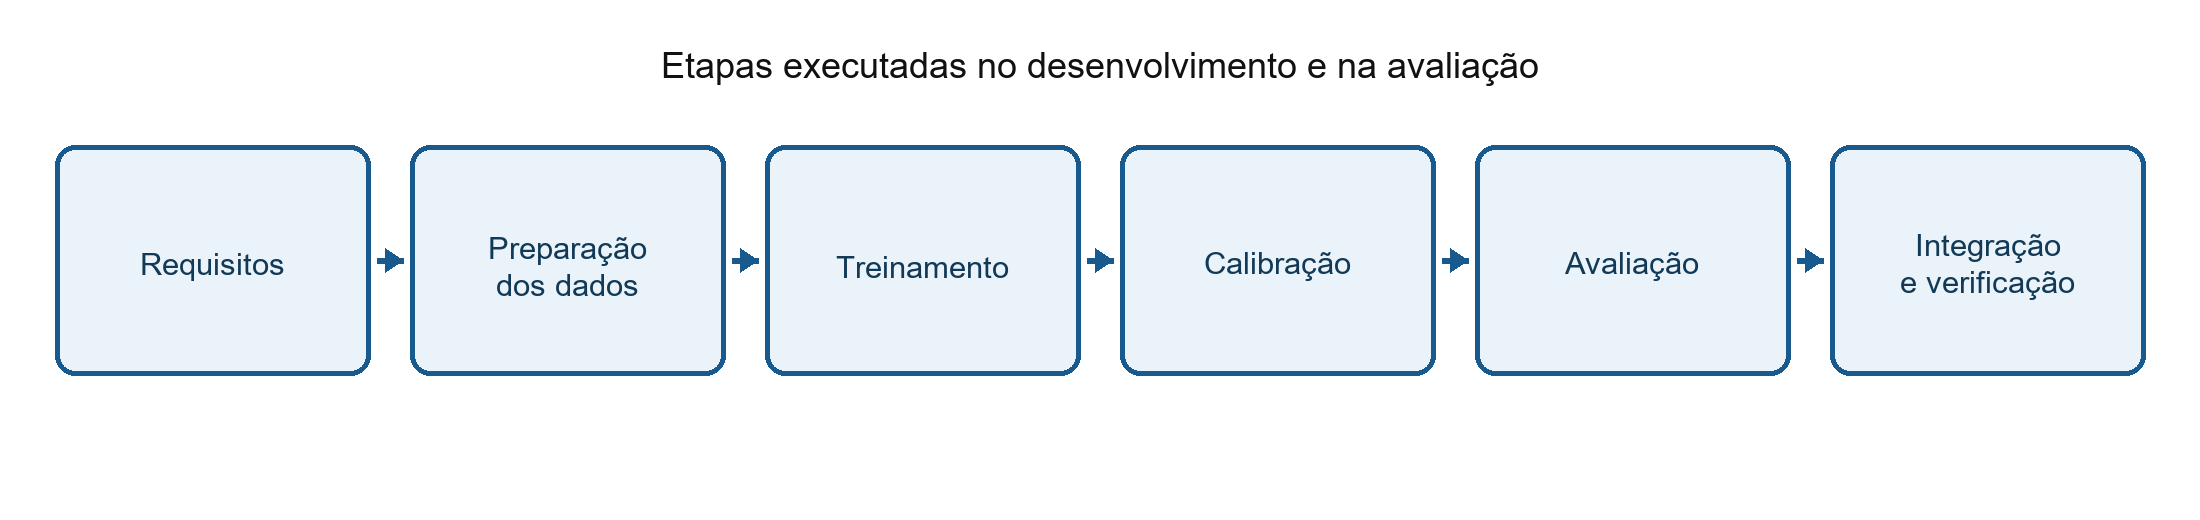
\includegraphics[width=13.60cm,height=0.72\textheight,keepaspectratio]{images/figura_11.png}\par
{\fontsize{10}{12}\selectfont Fonte: Elaborado pelo autor (2026).\par}
\end{figure}
\Needspace{12\baselineskip}\section{Levantamento de Requisitos}
O levantamento de requisitos foi conduzido por revisão bibliográfica sobre análise computacional de EEG, análise documental do formato EDF, estudo do fluxo proposto no projeto anterior e refinamentos realizados durante a orientação acadêmica.

Foram priorizados requisitos de ingestão, processamento de registros multicanais, visualização temporal, segurança, persistência e interpretabilidade. Não foram realizadas entrevistas estruturadas nem validação formal com neurologistas; por isso, os requisitos clínicos da versão atual são tratados como requisitos de um protótipo acadêmico.

O benchmarking teve caráter bibliográfico e conceitual. Foram comparadas características descritas na literatura e em ferramentas de processamento de EEG, com atenção a visualização, seleção de canais, suporte a EDF e explicabilidade. Ferramentas que não tenham sido avaliadas de forma documentada não são apresentadas como objetos de comparação empírica.

Como resultado, foram definidos os módulos de autenticação, pacientes, ingestão de EDF, visualização multicanal, análise preditiva, explicabilidade, configurações e emissão de laudo. A validação desses requisitos com profissionais da neurologia permanece como trabalho futuro.

\Needspace{12\baselineskip}\section{Desenvolvimento}
O desenvolvimento foi conduzido em ciclos incrementais individuais de implementação, teste e revisão. A orientação acadêmica apoiou a avaliação das entregas e o Git registrou a evolução do código. Nos ciclos de IA, hiperparâmetros e arquiteturas foram comparados por experimentos controlados antes da integração.

O sistema utiliza arquitetura full-stack orientada a serviços, separando o cliente React do servidor FastAPI. Essa separação mantém responsabilidades claras e permite que o processamento matemático ocorra no backend sem transferir os arquivos brutos ou o modelo para o navegador.

\Needspace{12\baselineskip}\section{Tecnologias e ferramentas utilizadas}
A implementação utilizou ferramentas com versões registradas para favorecer a reprodutibilidade do ambiente.

O backend foi desenvolvido com Python 3.11.9, FastAPI 0.115.6 e SQLAlchemy 2.0.36. Na configuração final, o PostgreSQL realiza a persistência relacional; EDFs, modelos e mapas permanecem no sistema de arquivos. A conexão com a API e a leitura dos registros foram verificadas após a migração dos dados locais. O ambiente Python é isolado por venv.

O frontend foi desenvolvido com React 19.2.7, TypeScript, Vite 6.3.5 e Recharts 3.9.0. O Recharts foi adotado por sua integração declarativa com React; D3.js não integra a versão final do protótipo.

O pipeline utiliza TensorFlow 2.16.2, MNE-Python 1.8.0, NumPy 1.26.4 e SHAP 0.46.0. O Git registra as alterações e o arquivo de dependências do Python, juntamente com o package-lock do frontend, apoia a reprodução do ambiente. Docker não foi adotado nesta versão.

\Needspace{12\baselineskip}\section{Desenvolvimento incremental}
A implementação foi dividida em incrementos dependentes, mas com atividades parcialmente paralelas. Cada incremento recebeu critérios objetivos de aceite:

\begin{itemize}[leftmargin=1.25cm,itemsep=0pt,topsep=0pt]
\item Incremento I (Infraestrutura e Ingestão): concluído quando a API passou a autenticar usuários, cadastrar pacientes, receber, validar, armazenar e ler arquivos EDF, extraindo canais e taxa de amostragem.
\item Incremento II (Núcleo de Inteligência): o extrator histórico implementou Entropia de Shannon e medidas de Dinâmica Simbólica, que foram investigadas como alternativas de representação. Após os experimentos, a CNN-BiLSTM final passou a receber 15 características tempo-frequência por canal, incluindo entropia espectral, mas não aquelas características históricas. A rede produz escores de suspeita ictal por passo temporal. A separação dos grupos ocorreu antes do janelamento e da amostragem.
\item Incremento III (Interface e Explicabilidade): concluído com a integração entre backend e frontend, incluindo visualização multicanal, seleção de canais, trechos suspeitos, sobreposição SHAP, configurações médicas e emissão de laudo.
\end{itemize}
A cada ciclo foram executados testes automatizados e verificações sobre arquivos EDF reais. Alterações experimentais na IA somente foram promovidas quando apresentaram benefício no protocolo controlado de calibração.

\Needspace{12\baselineskip}\section{Testes}
A verificação contemplou o comportamento do software e a avaliação científica do modelo, mantendo métricas de janela, EDF, evento e localização temporal em níveis distintos.

\begin{itemize}[leftmargin=1.25cm,itemsep=0pt,topsep=0pt]
\item Dados e métricas de IA: a base final foi a CHB-MIT (Shoeb, 2009), com registros contínuos multicanais em EDF e anotações temporais das crises. Foram destinados ao treino 77 EDFs de 17 grupos de pacientes e à calibração 13 EDFs de chb16, chb19, chb20 e chb24. A separação ocorreu por paciente antes do janelamento. Foram avaliados precisão, sensibilidade e F1 por EDF e por evento, F1 localizado, IoU temporal e falsos alarmes por hora.
\item Desempenho e carga: o processamento ponta a ponta foi verificado em EDF real de longa duração. O tempo aceitável para uso clínico não foi definido por profissionais da área; portanto, o trabalho não adota um limite arbitrário. Uma avaliação formal deve registrar hardware, duração do exame, tempo total, uso de memória e concorrência.
\item Usabilidade e interpretabilidade: foram realizados testes técnicos da interface, do alinhamento temporal e da projeção do SHAP. Não foi conduzido estudo formal com médicos ou técnicos; essa ausência é apresentada como limitação e trabalho futuro.
\end{itemize}
Precisão é a fração de predições positivas corretas; sensibilidade (recall) é a fração dos casos positivos reais detectados; F1 é a média harmônica entre ambas (F1 = 2PR/(P+R), com P = precisão e R = recall). Na análise por EDF, cada arquivo constitui uma unidade. Na análise por evento, uma crise foi considerada detectada quando algum candidato válido apresentou simultaneamente pelo menos 1 segundo de interseção e sobreposição correspondente a 25\% da duração do evento real; candidatos válidos sem essa correspondência foram contabilizados como falsos alarmes. A métrica FA/h corresponde ao número desses falsos alarmes dividido pelas horas não ictais analisadas, isto é, a duração total descontados os intervalos anotados como crise.

A IoU temporal foi calculada pela razão entre a duração da interseção e a duração da união dos intervalos real e previsto. O F1 localizado não é um F1 calculado amostra a amostra: ele mantém o EDF como unidade, mas somente considera correta a predição positiva de um EDF ictal quando o trecho principal selecionado satisfaz os mesmos critérios de sobreposição temporal. Assim, essa métrica penaliza arquivos classificados como positivos cujo candidato principal foi posicionado fora da crise. Já o F1 por evento considera todas as crises anotadas e todos os candidatos válidos, razão pela qual pode divergir do F1 localizado.

Para explicitar as unidades utilizadas, as métricas por EDF são definidas nas Equações~\ref{eq:precisao} a~\ref{eq:f1}. VP indica arquivo ictal classificado como positivo, FP indica arquivo não ictal classificado como positivo e FN indica arquivo ictal classificado como negativo.
\begin{equation}\label{eq:precisao}
P=\frac{VP}{VP+FP}
\end{equation}
\begin{equation}\label{eq:recall}
R=\frac{VP}{VP+FN}
\end{equation}
\begin{equation}\label{eq:f1}
F_1=\frac{2PR}{P+R}
\end{equation}
Para intervalos $A$ (referência) e $B$ (previsão), com $|\cdot|$ representando duração, a sobreposição e a taxa de falsos alarmes são dadas por:
\begin{equation}\label{eq:iou}
\mathrm{IoU}(A,B)=\frac{|A\cap B|}{|A\cup B|}
\end{equation}
\begin{equation}\label{eq:fah}
\mathrm{FA/h}=\frac{N_{\mathrm{alarmes\ sem\ correspondencia}}}{T_{\mathrm{nao\ ictal}}/3600}.
\end{equation}
Na Equação~\ref{eq:fah}, o tempo é medido em segundos. No avaliador utilizado, a sensibilidade por evento é a quantidade de crises detectadas dividida pelo total de crises, e a precisão por evento é calculada como crises detectadas divididas pela soma de crises detectadas e falsos alarmes. Não há pareamento exclusivo um a um: dois candidatos que correspondam à mesma crise não são necessariamente penalizados como duplicatas. Essa convenção é mantida para interpretar os resultados históricos. Os intervalos de referência do avaliador são reconstruídos dos rótulos das janelas; portanto, seus limites temporais estão sujeitos à discretização do janelamento.

\Needspace{12\baselineskip}\section{Implementação}
A versão avaliada foi implantada localmente como protótipo de pesquisa, com frontend, API, banco de dados e artefatos de IA executados no ambiente de desenvolvimento.

A implantação em nuvem não foi validada. Embora a arquitetura permita execução em servidor, acesso remoto, escalabilidade, criptografia de transporte e operação multiusuário exigem configuração e avaliação próprias antes de qualquer uso externo.

A API disponibiliza documentação Swagger/OpenAPI gerada pelo FastAPI. O repositório também registra variáveis de configuração, comandos de treinamento, calibração, avaliação e verificação dos artefatos.

A avaliação utilizou registros públicos reais e desidentificados da CHB-MIT. Não foram coletados exames de hospital local nem recrutados participantes. Eventual estudo com dados identificáveis ou interação com pacientes e profissionais deverá ser submetido às instâncias éticas e institucionais aplicáveis.

\chapter{SOFTWARE}
\Needspace{12\baselineskip}\section{Descrição}
O software configura-se como um protótipo funcional de plataforma web de apoio à análise de EEG. Seu público-alvo potencial inclui neurologistas, neurofisiologistas e pesquisadores, mas a versão atual não foi validada clinicamente nem regularizada para uso assistencial. A proposta responde ao esforço envolvido na revisão de registros extensos e à necessidade de reunir visualização, análise computacional, explicabilidade e laudo em um fluxo único.

A plataforma recebe arquivos EDF vinculados ao paciente, extrai metadados e apresenta os canais em uma linha temporal interativa. O pipeline CNN-BiLSTM produz escores temporais de suspeita ictal e agrega sequências sobrepostas em trechos suspeitos. O Gradient SHAP estima a contribuição das características da sequência de pico, e a interface projeta as relevâncias positivas por canal e intervalo de segundos. Essa explicação não corresponde a uma atribuição por amostra bruta e deve ser interpretada como apoio à inspeção, não como justificativa fisiológica conclusiva.

\Needspace{12\baselineskip}\section{Levantamento de Requisitos}
A engenharia de requisitos baseou-se em revisão bibliográfica, análise documental do EDF, experiência do projeto anterior e refinamento com a orientação acadêmica. Não houve entrevista estruturada nem validação formal com neurologistas. Assim, os requisitos clínicos representam hipóteses de projeto para um protótipo e deverão ser avaliados com profissionais antes de uma eventual evolução assistencial.

\Needspace{12\baselineskip}\section{Requisitos Funcionais e Não Funcionais}
Conforme abordado por Sommerville (2011), a especificação de requisitos é um pilar fundamental da Engenharia de Software, definindo com clareza as expectativas dos usuários e as restrições operacionais sob as quais o sistema deve atuar. Os requisitos dividem-se tradicionalmente em funcionais, que estabelecem detalhadamente as ações declarativas, as reações a entradas específicas e os serviços explícitos que o software é obrigado a executar, e requisitos não funcionais, os quais não se ligam diretamente aos serviços individuais do sistema, mas sim às propriedades emergentes de qualidade, confiabilidade, desempenho, compatibilidade e segurança corporativa.

A partir da análise estrutural da plataforma e do pipeline de triagem neurofisiológica estabelecido na metodologia, foram definidos os seguintes requisitos de engenharia para o sistema:

\textbf{Requisitos Funcionais:}

\noindent \textbf{1 – Autenticar Usuário:} O sistema deve fornecer uma interface de login para que o médico neurologista insira suas credenciais e acesse a plataforma de forma restrita.\par
\noindent \textbf{2 – Gerenciar Pacientes:} O sistema deve permitir a inclusão, alteração, consulta e exclusão de dados cadastrais básicos e prontuários clínicos dos pacientes.\par
\noindent \textbf{3 – Importar Exame (.EDF):} O sistema deve fornecer mecanismos para o upload e a ingestão de arquivos de sinais biomédicos estruturados no formato padrão universal .EDF.\par
\noindent \textbf{4 – Extrair Metadados do Sinal:} O sistema deve decodificar o cabeçalho (header) do arquivo binário carregado e extrair automaticamente informações como taxa de amostragem e os rótulos dos canais de eletrodos.\par
\noindent \textbf{5 – Visualizar Sinais de EEG:} O sistema deve plotar graficamente na tela do usuário as séries temporais contínuas e multicanais correspondentes às ondas cerebrais captadas.\par
\noindent \textbf{6 – Manipulação Interativa de Ondas:} O sistema deve permitir que o médico execute comandos responsivos de zoom horizontal e vertical e isole montagens de canais focais diretamente no painel.\par
\noindent \textbf{7 – Solicitar Análise Preditiva: }O sistema deve acionar o modelo CNN-BiLSTM sobre um exame EDF já importado para gerar escores de suspeita ictal por intervalo e destacar trechos para revisão médica.\par
\noindent \textbf{8 – Exibir Justificativa Visual (XAI): }O sistema deve sobrepor um mapa de calor gerado com os valores do algoritmo SHAP sobre o traçado original do EEG, destacando em vermelho os intervalos e canais que contribuíram para o escore da rede neural.\par
\noindent \textbf{9 – Emitir Laudo Médico:} O sistema deve disponibilizar um campo de texto descritivo para que o especialista redija e formalize o laudo definitivo do exame, integrando a triagem analítica.\par
\textbf{Requisitos Não Funcionais:}

\noindent \textbf{1 – Desempenho (Processamento Assíncrono):} A execução do pipeline de engenharia de features matemáticas e inferência da rede neural profunda não deve bloquear ou congelar a interface de visualização do usuário (client-side).\par
\noindent \textbf{2 – Compatibilidade e Portabilidade:} O software deve ser executado e renderizado com total fidelidade diretamente através de navegadores web modernos compatíveis com os padrões HTML5 e JavaScript.\par
\noindent \textbf{3 – Segurança e Privacidade: }O sistema deve restringir rotas clínicas a usuários autenticados, armazenar senhas por hash e evitar exposição desnecessária de dados. A versão atual não implementa consentimento, política automatizada de retenção, criptografia específica dos EDF em repouso ou trilha completa de auditoria; esses controles são necessários antes do uso com dados identificáveis.\par
\noindent \textbf{4 – Usabilidade e Responsividade:} A interface analítica deve ser projetada com foco em ergonomia e usabilidade médica, garantindo a exibição fluida e nítida das séries temporais de alta densidade em monitores de alta resolução.\par
\noindent \textbf{5 – Confiabilidade e Robustez de I/O:} A arquitetura de persistência híbrida deve suportar o armazenamento íntegro e a rápida velocidade de entrada e saída (I/O) exigida por arquivos pesados de Big Data na saúde.\par
\Needspace{12\baselineskip}\section{Casos de uso}
Segundo Pressman e Maxim (2016), os casos de uso descrevem as interações entre atores e funcionalidades do sistema. Neste protótipo, o médico é o ator principal; a extração de características e a inferência são operações internas acionadas após a solicitação de análise de um exame previamente importado.

Ao solicitar a análise preditiva, o médico seleciona um exame previamente importado. A extração de métricas e a execução do modelo constituem operações internas obrigatórias do sistema, e não casos de uso iniciados diretamente pelo médico. A visualização da explicação permanece opcional durante a revisão do resultado.

\begin{figure}[htbp]
\centering
\caption{Diagrama de Casos de Uso da Plataforma Web.}
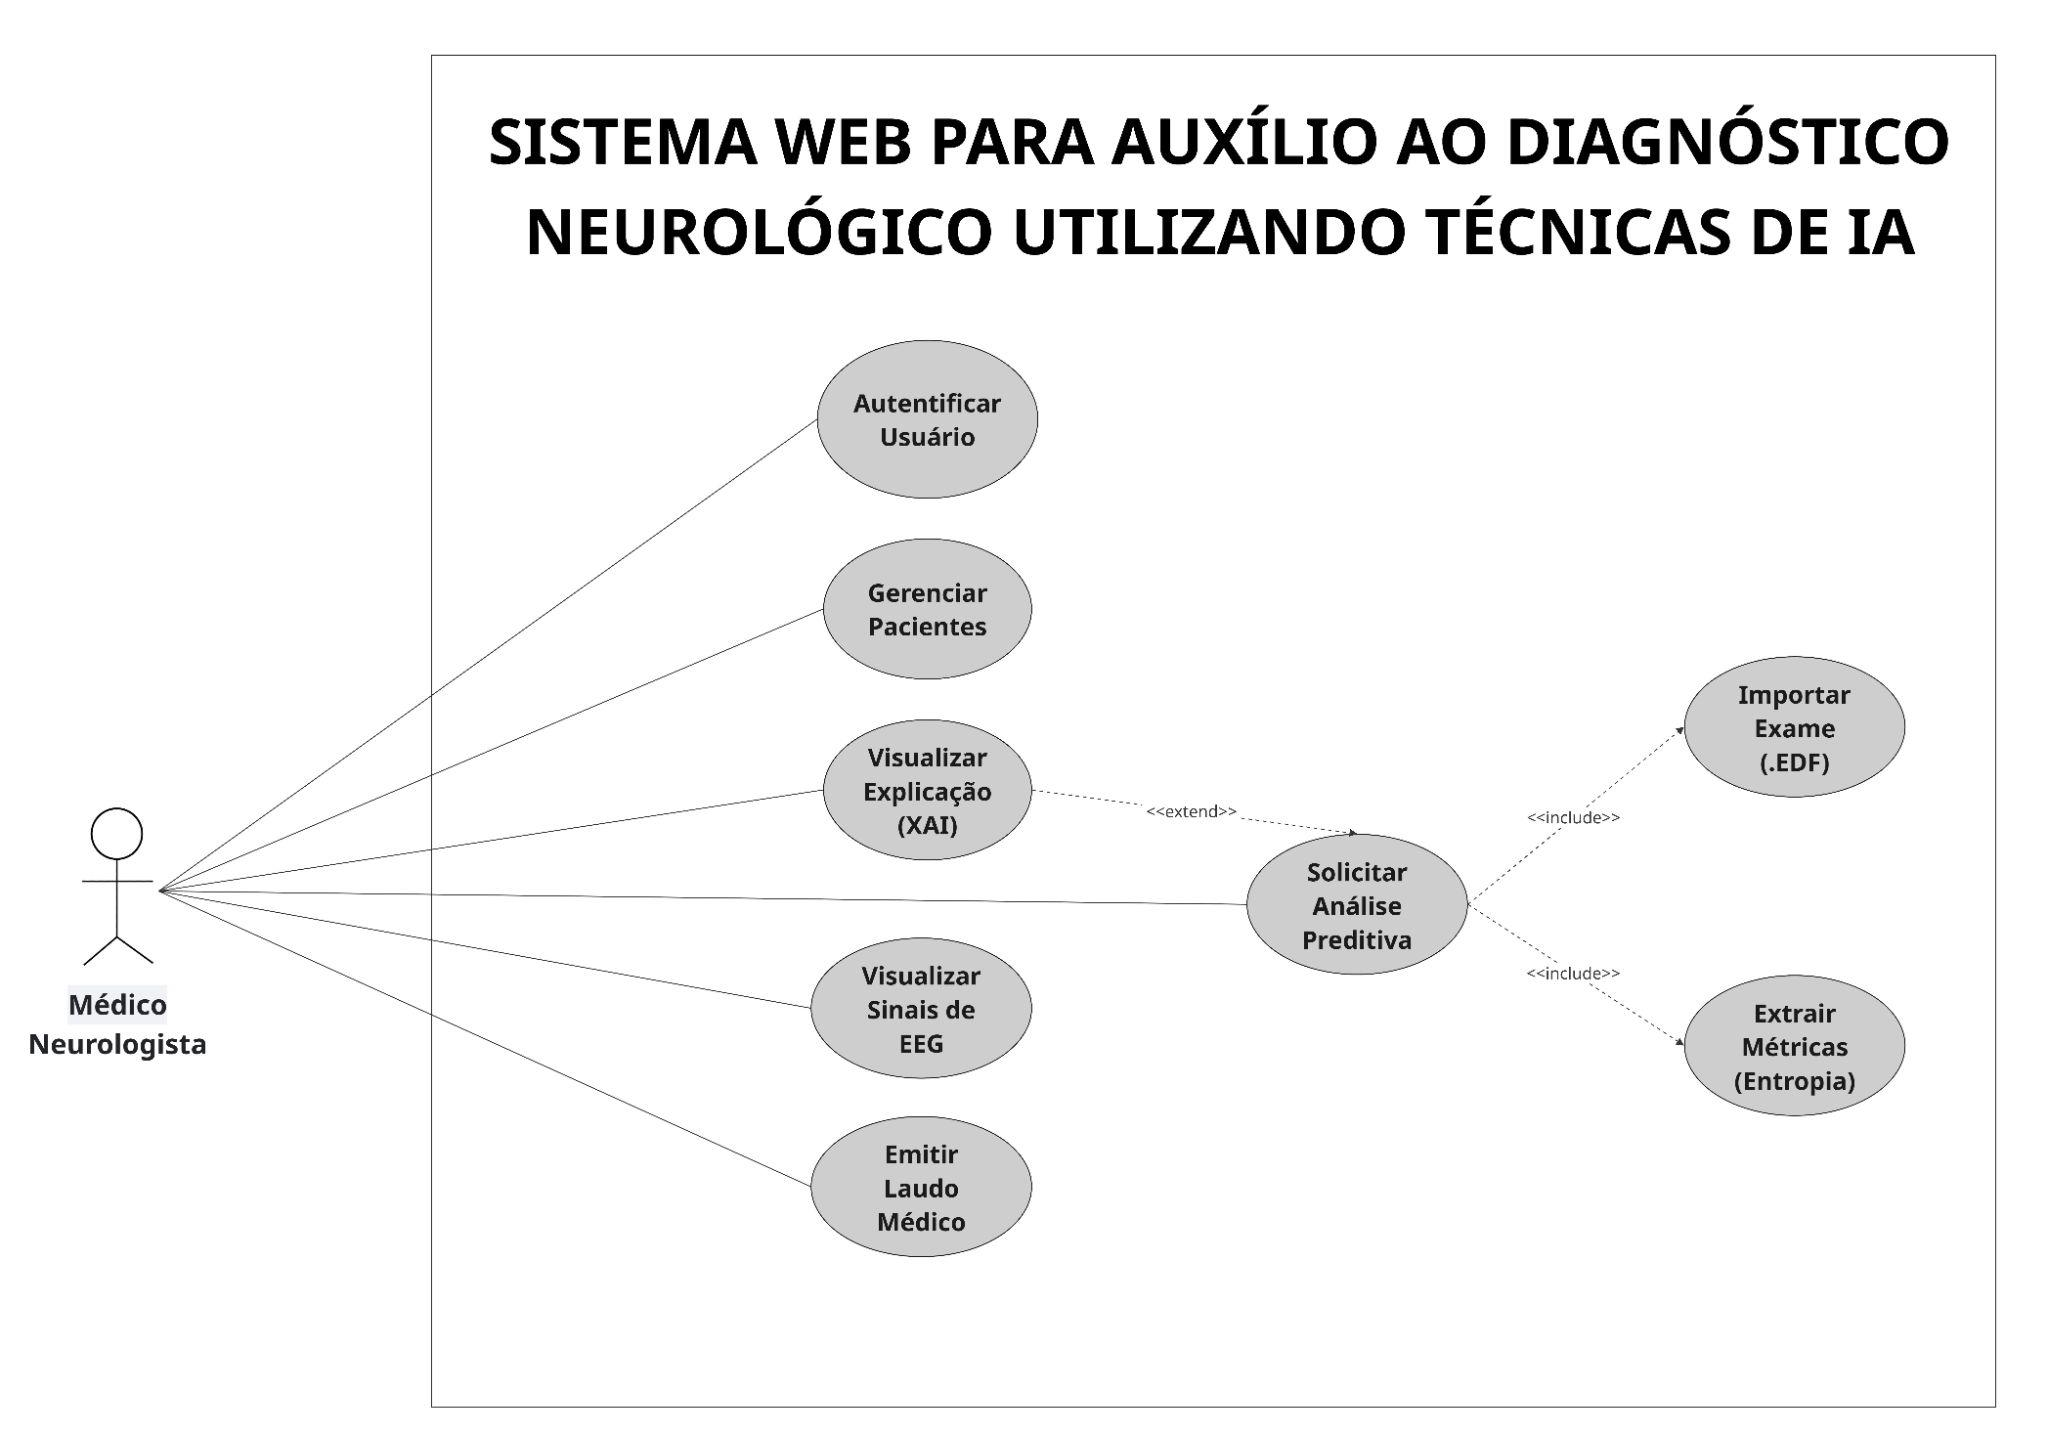
\includegraphics[width=13.60cm,height=0.72\textheight,keepaspectratio]{images/figura_01.jpg}\par
{\fontsize{10}{12}\selectfont Fonte: Elaborado pelo autor (2026).\par}
\end{figure}
\FloatBarrier\Needspace{9\baselineskip}
\captionof{table}{Documentação do caso de uso: Autenticar Usuário}\nopagebreak[4]
\begingroup
\fontsize{10}{12}\selectfont
\setlength{\tabcolsep}{3pt}
\renewcommand{\arraystretch}{1.15}
\addtocounter{table}{-1}
\begin{longtable}{|>{\raggedright\arraybackslash}p{0.460\textwidth}|>{\raggedright\arraybackslash}p{0.460\textwidth}|}
\hline
\textbf{Nome do caso de uso} & \textbf{Autenticar Usuário} \\ \hline
\endfirsthead
\hline
\textbf{Nome do caso de uso} & \textbf{Autenticar Usuário} \\ \hline
\endhead
Caso de uso geral & - \\ \hline
Ator principal & Médico Neurologista \\ \hline
Atores secundários & - \\ \hline
Resumo & Este caso de uso descreve o processo de autenticação de segurança, permitindo que o médico insira suas credenciais para obter acesso seguro ao painel de controle da plataforma. \\ \hline
Pré-condições & O médico deve estar previamente cadastrado no banco de dados do sistema. \\ \hline
Pós-condições & O usuário é autenticado, um token de sessão JWT é gerado e o painel principal é carregado no frontend. \\ \hline
Ações do ator & Ações do sistema \\ \hline
1 – Acessar a tela inicial da plataforma web e preencher os campos de e-mail e senha. &  \\ \hline
 & 2 – Receber os dados de login através da API FastAPI de forma assíncrona. \\ \hline
3 – Clicar no botão "Entrar". &  \\ \hline
 & 4 – Validar as credenciais comparando a senha informada com o hash criptográfico armazenado no PostgreSQL. Se válidas, liberar o acesso à área restrita. \\ \hline
Restrições/Validações & 1 – Não permitir campos em branco no formulário de login. \\ \hline
Restrições/Validações & 2 – Bloquear a autenticação caso a combinação de e-mail e senha seja inválida. \\ \hline
\end{longtable}
\endgroup
\nopagebreak[4]{\centering\fontsize{10}{12}\selectfont Fonte: Elaborado pelo autor (2026).\par}
\FloatBarrier\Needspace{9\baselineskip}
\captionof{table}{Documentação do caso de uso: Gerenciar Pacientes}\nopagebreak[4]
\begingroup
\fontsize{10}{12}\selectfont
\setlength{\tabcolsep}{3pt}
\renewcommand{\arraystretch}{1.15}
\addtocounter{table}{-1}
\begin{longtable}{|>{\raggedright\arraybackslash}p{0.460\textwidth}|>{\raggedright\arraybackslash}p{0.460\textwidth}|}
\hline
\textbf{Nome do caso de uso} & \textbf{Gerenciar Pacientes} \\ \hline
\endfirsthead
\hline
\textbf{Nome do caso de uso} & \textbf{Gerenciar Pacientes} \\ \hline
\endhead
Caso de uso geral & - \\ \hline
Ator principal & Médico Neurologista \\ \hline
Atores secundários & - \\ \hline
Resumo & Este caso de uso descreve o processo de inclusão, alteração ou consulta dos dados cadastrais e prontuários médicos dos pacientes na plataforma. \\ \hline
Pré-condições & O médico deve estar devidamente autenticado no sistema. \\ \hline
Pós-condições & Os registros do paciente são atualizados ou salvos de maneira consistente no banco de dados relacional. \\ \hline
Ações do ator & Ações do sistema \\ \hline
1 – Selecionar a opção de menu "Pacientes" e clicar em "Novo Cadastro". &  \\ \hline
 & 2 – Exibir o formulário de cadastro de paciente na interface React.js. \\ \hline
3 – Preencher as informações obrigatórias (Nome, Data de Nascimento, Gênero e CPF) e clicar em "Salvar". &  \\ \hline
 & 4 – Validar a integridade das informações e persistir os dados na tabela correspondente do PostgreSQL, exibindo mensagem de sucesso. \\ \hline
Restrições/Validações & 1 – Impedir a gravação de dados caso o CPF informado seja inválido ou já conste no sistema. \\ \hline
Restrições/Validações & 2 – Validar se os campos obrigatórios foram preenchidos corretamente. \\ \hline
\end{longtable}
\endgroup
\nopagebreak[4]{\centering\fontsize{10}{12}\selectfont Fonte: Elaborado pelo autor (2026).\par}
\FloatBarrier\Needspace{9\baselineskip}
\captionof{table}{Documentação do caso de uso: Importar Exame (.EDF)}\nopagebreak[4]
\begingroup
\fontsize{10}{12}\selectfont
\setlength{\tabcolsep}{3pt}
\renewcommand{\arraystretch}{1.15}
\addtocounter{table}{-1}
\begin{longtable}{|>{\raggedright\arraybackslash}p{0.460\textwidth}|>{\raggedright\arraybackslash}p{0.460\textwidth}|}
\hline
\textbf{Nome do caso de uso} & \textbf{Importar Exame (.EDF)} \\ \hline
\endfirsthead
\hline
\textbf{Nome do caso de uso} & \textbf{Importar Exame (.EDF)} \\ \hline
\endhead
Caso de uso geral & - \\ \hline
Ator principal & Médico Neurologista \\ \hline
Atores secundários & - \\ \hline
Resumo & Este caso de uso descreve a ingestão de arquivos biomédicos padronizados no formato .EDF para o servidor, vinculando o exame ao prontuário do paciente selecionado. \\ \hline
Pré-condições & O médico deve estar autenticado e o paciente correspondente selecionado em tela. \\ \hline
Pós-condições & O arquivo binário do exame é armazenado no sistema de arquivos estruturado e seus metadados são indexados no banco de dados. \\ \hline
Ações do ator & Ações do sistema \\ \hline
1 – Clicar na opção "Importar Novo Exame" dentro do perfil do paciente. &  \\ \hline
 & 2 – Abrir a caixa de seleção de arquivos locais do sistema operacional. \\ \hline
3 – Selecionar o arquivo com extensão .edf desejado e confirmar o envio. &  \\ \hline
 & 4 – Transferir o arquivo via requisição Multipart e executar o processamento assíncrono do cabeçalho (header) do arquivo via biblioteca MNE-Python, extraindo canais e taxa de amostragem. \\ \hline
Restrições/Validações & 1 – Recusar arquivos que não possuam estritamente a extensão .edf. \\ \hline
Restrições/Validações & 2 – Verificar a integridade do cabeçalho binário do arquivo para atestar que o sinal não está corrompido antes do salvamento. \\ \hline
\end{longtable}
\endgroup
\nopagebreak[4]{\centering\fontsize{10}{12}\selectfont Fonte: Elaborado pelo autor (2026).\par}
\FloatBarrier\Needspace{9\baselineskip}
\captionof{table}{Documentação do caso de uso: Visualizar Sinais de EEG}\nopagebreak[4]
\begingroup
\fontsize{10}{12}\selectfont
\setlength{\tabcolsep}{3pt}
\renewcommand{\arraystretch}{1.15}
\addtocounter{table}{-1}
\begin{longtable}{|>{\raggedright\arraybackslash}p{0.460\textwidth}|>{\raggedright\arraybackslash}p{0.460\textwidth}|}
\hline
\textbf{Nome do caso de uso} & \textbf{Visualizar Sinais de EEG} \\ \hline
\endfirsthead
\hline
\textbf{Nome do caso de uso} & \textbf{Visualizar Sinais de EEG} \\ \hline
\endhead
Caso de uso geral & - \\ \hline
Ator principal & Médico Neurologista \\ \hline
Atores secundários & - \\ \hline
Resumo & Este caso de uso descreve a plotagem gráfica e interativa das séries temporais multicanais das ondas cerebrais de EEG na interface web do usuário. \\ \hline
Pré-condições & O arquivo do exame já deve ter sido importado com sucesso na plataforma. \\ \hline
Pós-condições & Os traçados de sinais elétricos são exibidos de forma reativa e fluida em tela, permitindo manipulações visuais pelo usuário. \\ \hline
Ações do ator & Ações do sistema \\ \hline
1 – Selecionar o exame de EEG correspondente na linha do tempo do paciente. &  \\ \hline
 & 2 – Buscar os blocos de vetores temporais do arquivo de sinais e renderizar os canais na tela usando os componentes gráficos da aplicação. \\ \hline
3 – Executar interações na tela, como comandos de zoom horizontal/vertical e seleção dinâmica de montagens de canais específicos. &  \\ \hline
 & 4 – Atualizar as escalas dos eixos, recalculando a renderização visual das ondas cerebrais em tempo real conforme os filtros acionados. \\ \hline
Restrições/Validações & 1 – O sistema deve limitar a quantidade de pontos simultâneos renderizados na tela para evitar gargalos de memória e travamentos na interface React.js. \\ \hline
\end{longtable}
\endgroup
\nopagebreak[4]{\centering\fontsize{10}{12}\selectfont Fonte: Elaborado pelo autor (2026).\par}
\FloatBarrier\Needspace{9\baselineskip}
\captionof{table}{Documentação do caso de uso: Solicitar Análise Preditiva}\nopagebreak[4]
\begingroup
\fontsize{10}{12}\selectfont
\setlength{\tabcolsep}{3pt}
\renewcommand{\arraystretch}{1.15}
\addtocounter{table}{-1}
\begin{longtable}{|>{\raggedright\arraybackslash}p{0.460\textwidth}|>{\raggedright\arraybackslash}p{0.460\textwidth}|}
\hline
\textbf{Nome do caso de uso} & \textbf{Solicitar Análise Preditiva} \\ \hline
\endfirsthead
\hline
\textbf{Nome do caso de uso} & \textbf{Solicitar Análise Preditiva} \\ \hline
\endhead
Caso de uso geral & - \\ \hline
Ator principal & Médico Neurologista \\ \hline
Atores secundários & - \\ \hline
Resumo & Este caso de uso detalha o acionamento do pipeline de inteligência artificial para realizar a triagem temporal e destacar segmentos com atividade compatível com os eventos ictais aprendidos a partir das anotações da CHB-MIT. \\ \hline
Pré-condições & O arquivo EDF correspondente deve estar previamente importado e carregado no backend. \\ \hline
Pós-condições & Os escores temporais, os trechos suspeitos e os metadados da análise são persistidos e disponibilizados na interface. \\ \hline
Ações do ator & Ações do sistema \\ \hline
1 – Clicar no comando "Solicitar Análise da IA" localizado no painel de visualização do exame. &  \\ \hline
 & 2 – Extrair 15 características tempo-frequência por canal e por janela, incluindo entropia espectral, para formar sequências temporais. \\ \hline
 & 3 – Alimentar a rede CNN-BiLSTM com as sequências de características para estimar o escore de suspeita ictal em cada passo temporal. \\ \hline
 & 4 – Persistir o resultado e destacar graficamente no painel os trechos que devem ser revisados pelo especialista. \\ \hline
Restrições/Validações & 1 – Executar a análise em segundo plano para que a requisição inicial não permaneça bloqueada durante todo o processamento. \\ \hline
\end{longtable}
\endgroup
\nopagebreak[4]{\centering\fontsize{10}{12}\selectfont Fonte: Elaborado pelo autor (2026).\par}
\FloatBarrier\Needspace{9\baselineskip}
\captionof{table}{Documentação do caso de uso: Visualizar Explicação (XAI)}\nopagebreak[4]
\begingroup
\fontsize{10}{12}\selectfont
\setlength{\tabcolsep}{3pt}
\renewcommand{\arraystretch}{1.15}
\addtocounter{table}{-1}
\begin{longtable}{|>{\raggedright\arraybackslash}p{0.460\textwidth}|>{\raggedright\arraybackslash}p{0.460\textwidth}|}
\hline
\textbf{Nome do caso de uso} & \textbf{Visualizar Explicação (XAI)} \\ \hline
\endfirsthead
\hline
\textbf{Nome do caso de uso} & \textbf{Visualizar Explicação (XAI)} \\ \hline
\endhead
Caso de uso geral & - \\ \hline
Ator principal & Médico Neurologista \\ \hline
Atores secundários & - \\ \hline
Resumo & Este caso de uso descreve a exibição das contribuições computacionais estimadas pelo Gradient SHAP para a sequência de pico analisada pela rede neural. \\ \hline
Pré-condições & A análise preditiva descrita no Quadro 5 deve estar concluída e possuir uma sequência de pico válida. \\ \hline
Pós-condições & Gráficos explicativos com mapas de calor coloridos são sobrepostos às ondas de EEG para inspeção do médico. \\ \hline
Ações do ator & Ações do sistema \\ \hline
1 – Acionar a opção de exibição do mapa SHAP no painel de resultados preditivos. &  \\ \hline
 & 2 – Associar os valores positivos de Gradient SHAP às features, aos canais e aos intervalos temporais da sequência de pico. \\ \hline
 & 3 – Projetar as relevâncias por canal e intervalo de segundos sobre o traçado exibido, mantendo explícito que a explicação não é calculada por amostra bruta. \\ \hline
Restrições/Validações & 1 – O mapa deve utilizar o mesmo mapeamento de sequência, passo temporal, canais e intervalos empregado na inferência da sequência de pico. A seleção de outro candidato na interface não recalcula automaticamente uma nova explicação SHAP. \\ \hline
\end{longtable}
\endgroup
\nopagebreak[4]{\centering\fontsize{10}{12}\selectfont Fonte: Elaborado pelo autor (2026).\par}
\FloatBarrier\Needspace{9\baselineskip}
\captionof{table}{Documentação do caso de uso: Emitir Laudo Médico}\nopagebreak[4]
\begingroup
\fontsize{10}{12}\selectfont
\setlength{\tabcolsep}{3pt}
\renewcommand{\arraystretch}{1.15}
\addtocounter{table}{-1}
\begin{longtable}{|>{\raggedright\arraybackslash}p{0.460\textwidth}|>{\raggedright\arraybackslash}p{0.460\textwidth}|}
\hline
\textbf{Nome do caso de uso} & \textbf{Emitir Laudo Médico} \\ \hline
\endfirsthead
\hline
\textbf{Nome do caso de uso} & \textbf{Emitir Laudo Médico} \\ \hline
\endhead
Caso de uso geral & - \\ \hline
Ator principal & Médico Neurologista \\ \hline
Atores secundários & - \\ \hline
Resumo & Este caso de uso descreve o processo de conclusão do exame, permitindo que o especialista insira seu parecer final baseando-se em suas conclusões e na segunda opinião fornecida pela IA. \\ \hline
Pré-condições & O médico deve ter revisado as análises visuais e preditivas geradas no prontuário do paciente. \\ \hline
Pós-condições & O laudo clínico final é salvo em formato definitivo e o status do exame é modificado para "Concluído". \\ \hline
Ações do ator & Ações do sistema \\ \hline
1 – Acessar o campo de digitação textual para o laudo médico final. &  \\ \hline
2 – Digitar as impressões clínicas e decidir se confirma ou desconsidera os alertas emitidos pela triagem do algoritmo inteligente. &  \\ \hline
3 – Clicar na ação "Emitir Laudo Finalizado". & 4 – Salvar o texto associado ao exame, alterar o status para Concluído e impedir novas edições. \\ \hline
Restrições/Validações & 1 – Impedir a emissão se o texto estiver vazio. 2 – Informar que não há rascunho persistente, campos estruturados ou assinatura digital nesta versão. \\ \hline
\end{longtable}
\endgroup
\nopagebreak[4]{\centering\fontsize{10}{12}\selectfont Fonte: Elaborado pelo autor (2026).\par}
\Needspace{12\baselineskip}\section{Arquitetura do Sistema}
A aplicação adota uma organização cliente-servidor: a interface React se comunica com a API FastAPI por HTTP, enquanto o servidor mantém as regras de negócio, a persistência e o processamento de EEG. Essa separação facilita a manutenção dos componentes (Richards, 2015). A análise de IA é solicitada separadamente após a importação do EDF e executada em segundo plano.

O frontend é uma aplicação React e TypeScript. O traçado multicanal utiliza Recharts e oferece navegação temporal, seleção de canais e sobreposição de trechos suspeitos. O backend, em Python e FastAPI, utiliza MNE-Python na leitura do EDF e TensorFlow/Keras na inferência da CNN-BiLSTM. Os metadados são persistidos no PostgreSQL configurado para a versão final.

Após o envio do EDF, a API valida e armazena o arquivo e registra o exame. Quando o médico solicita a análise, o pipeline extrai 15 características por canal em janelas temporais e forma sequências para a CNN-BiLSTM, que produz escores de suspeita ictal ao longo do tempo. A explicação Gradient SHAP é calculada para a sequência de pico e projetada por canal e intervalo de segundos na interface. Essa projeção não atribui relevância a cada amostra bruta do sinal e não substitui a interpretação médica.

\Needspace{12\baselineskip}\section{Fluxograma}
Para mapear de maneira lógica a dinâmica operacional e a rastreabilidade dos dados na plataforma web proposta, desenvolveu-se o fluxograma detalhado na Figura 3. Conforme preconizado pelas boas práticas de Engenharia de Software, o fluxo foi segmentado visualmente em três macrocamadas interdependentes e síncronas/assíncronas, diferenciadas por meio de uma paleta de cores funcional para facilitar a compreensão da arquitetura lógica do sistema:

\begin{itemize}[leftmargin=1.25cm,itemsep=0pt,topsep=0pt]
\item Camada de Interface (Em Azul): Representa o frontend em React.js, sendo a camada de interação direta do médico neurologista com o sistema.
\item Camada de Servidor (Em Verde): Representa o backend FastAPI, responsável pela lógica de negócio, validação dos arquivos e persistência dos metadados no PostgreSQL.
\item Camada de Pipeline de IA (Em Roxo): Representa o motor de processamento matemático e inferência de redes neurais profundas em Python.
\end{itemize}
A lógica de processamento mapeada no diagrama cumpre rigorosamente quatro fases sequenciais estruturadas:

\textbf{1. Autenticação e Gestão Cadastral: }O fluxo inicia-se com a validação das credenciais do usuário na tela de login. Na busca pelo prontuário, caso o paciente pesquisado via CPF não conste na base, a interface força o redirecionamento para um formulário de cadastro simplificado, assegurando as restrições de integridade referencial antes da abertura do exame.

\textbf{2. Ingestão e Validação de Arquivo:} O arquivo biomédico com extensão .EDF é submetido pela interface via requisição HTTP POST Multipart. O servidor FastAPI intercepta o arquivo e valida a integridade do seu cabeçalho (header); caso haja inconformidade ou erro de formato, o fluxo é interrompido com uma notificação de erro ao cliente, impedindo a persistência de dados corrompidos.

\textbf{3. Processamento Inteligente em Segundo Plano: }Após a importação, o médico solicita a análise do exame. O servidor executa em segundo plano a extração das 15 características por canal e a inferência CNN-BiLSTM. Os escores são agregados em trechos temporais suspeitos; o SHAP estima as contribuições para a sequência de pico. Os metadados e resultados são registrados no banco relacional configurado, enquanto EDF e imagens permanecem em disco.

Na Figura 3, os blocos roxos representam o pipeline conceitual definido no planejamento inicial. Na implementação final, essas etapas foram consolidadas na extração de 15 características tempo-frequência por canal e na inferência temporal pela rede CNN-BiLSTM.

\textbf{4. Conclusão Clínico-Administrativa: }A interface apresenta o EEG, os trechos suspeitos e, quando disponível, a relevância SHAP por canal e intervalo. O médico pode registrar seu parecer no laudo. A saída da IA é apoio à revisão, não diagnóstico autônomo.

\begin{figure}[htbp]
\centering
\caption{Fluxograma de Execução e Ciclo de Vida dos Dados da Plataforma.}
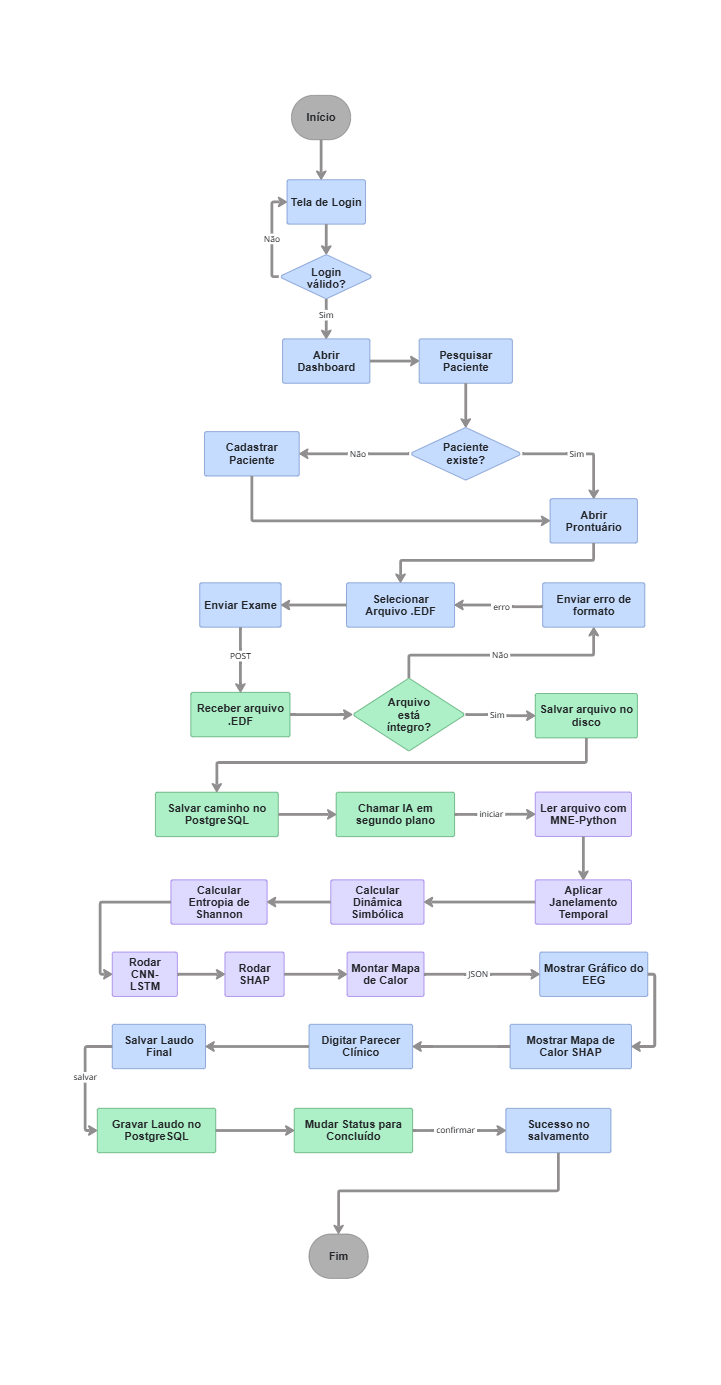
\includegraphics[width=8.47cm,height=0.72\textheight,keepaspectratio]{images/figura_03.png}\par
{\fontsize{10}{12}\selectfont Fonte: Elaborado pelo autor (2026).\par}
\end{figure}
\Needspace{12\baselineskip}\section{Modelo Entidade Relacionamento}
Conforme abordado por Elmasri e Navathe (2011), o Modelo Entidade-Relacionamento (MER) consiste em uma técnica de modelagem conceitual de alto nível amplamente utilizada no design de bancos de dados, permitindo mapear de forma abstrata as estruturas de dados e os requisitos de informação de um ecossistema de software. Essa abordagem viabiliza a representação visual do domínio do sistema por meio da identificação de entidades abstratas ou objetos do mundo real, de seus respectivos atributos qualificadores e dos relacionamentos lógicos estabelecidos entre essas estruturas.

Para representar a persistência implementada no protótipo, o modelo relaciona quatro entidades principais: Usuario, Paciente, Exame e Predicao\_IA. O texto do laudo permanece associado ao Exame, enquanto as saídas do modelo e a referência do SHAP são armazenadas em Predicao\_IA. Não existe entidade específica de auditoria na versão atual.

A entidade Usuario armazena dados profissionais e o hash da senha dos médicos autorizados. Paciente centraliza os dados cadastrais e se relaciona aos exames registrados. Embora o sistema possua autenticação, a implementação atual não equivale a conformidade integral com a LGPD.

A entidade Exame registra o arquivo EDF, os metadados extraídos, o estado do processamento e o texto livre do laudo. Depois da emissão, o laudo torna-se imutável. Não há rascunho persistente, campos clínicos estruturados ou assinatura digital nesta versão.

A entidade Predicao\_IA registra o resultado analítico, o escore, os trechos suspeitos e a referência do mapa SHAP. Arquivos EDF, modelos e imagens permanecem no sistema de arquivos e são referenciados pelo banco.

\begin{figure}[htbp]
\centering
\caption{Modelo Entidade Relacionamento.}
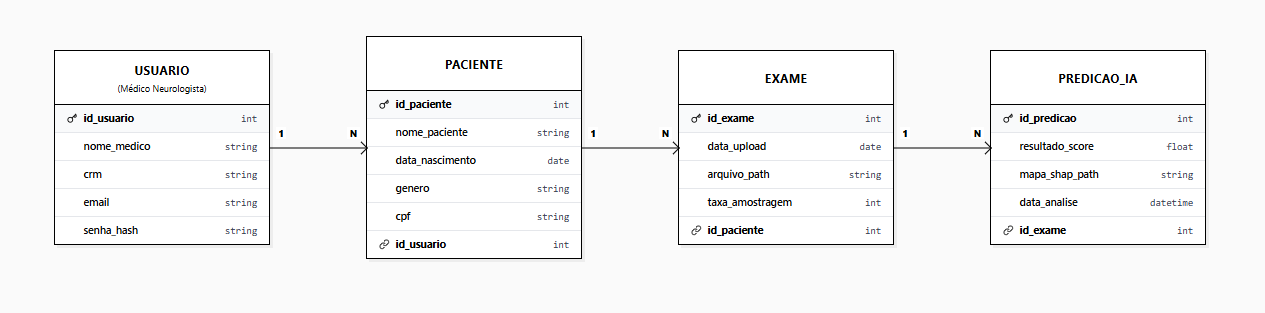
\includegraphics[width=13.60cm,height=0.72\textheight,keepaspectratio]{images/figura_02.png}\par
{\fontsize{10}{12}\selectfont Fonte: Elaborado pelo autor (2026).\par}
\end{figure}
\Needspace{12\baselineskip}\section{Protótipos de baixa fidelidade}
O desenvolvimento de Sistemas de Apoio à Decisão Clínica (SADC) exige uma atenção rigorosa à usabilidade e à interação, visto que a eficácia da ferramenta está diretamente ligada à capacidade do profissional de saúde em interpretar os dados de forma ágil, intuitiva e sem sobrecarga cognitiva. Antes de avançar para a implementação em código, a construção de interfaces de usuário (User Interfaces - UI) requer um planejamento visual rigoroso.

Para esse efeito, a utilização de wireframes e protótipos constitui uma ferramenta metodológica essencial. Segundo Pressman e Maxim (2016), a prototipação de telas permite que os programadores e os futuros usuários visualizem a disposição das informações, o fluxo de navegação e as funcionalidades primárias do software antes da fase de codificação final, mitigando riscos, retrabalho e falhas de comunicação.

Neste contexto, visando materializar a proposta da plataforma Web de apoio à análise neurológica desenvolvida neste projeto, foram elaborados wireframes que representam o fluxo de interação do especialista médico com o sistema. A concepção dessas interfaces teve como premissa principal integrar a complexidade da visualização de sinais de Eletroencefalograma (EEG) e os resultados preditivos do modelo de Inteligência Artificial Explicável (XAI) em um ambiente limpo e responsivo.

As figuras a seguir apresentam as principais telas projetadas, detalhando a jornada do usuário desde a autenticação no sistema, passando pela gestão de prontuários, até a área central de análise visual e emissão de laudos com o suporte da rede neural.

A Figura 5 apresenta a tela de login do sistema, porta de entrada para a plataforma de suporte à decisão clínica. Centralizada e com design minimalista, a interface conta com campos para a inserção do e-mail e da senha de acesso, além do botão de ação principal "Entrar no Sistema". O layout foi projetado com tipografia limpa, priorizando a legibilidade imediata e destacando no rodapé que o acesso é restrito aos profissionais credenciados.

\begin{figure}[htbp]
\centering
\caption{Tela de login do sistema.}
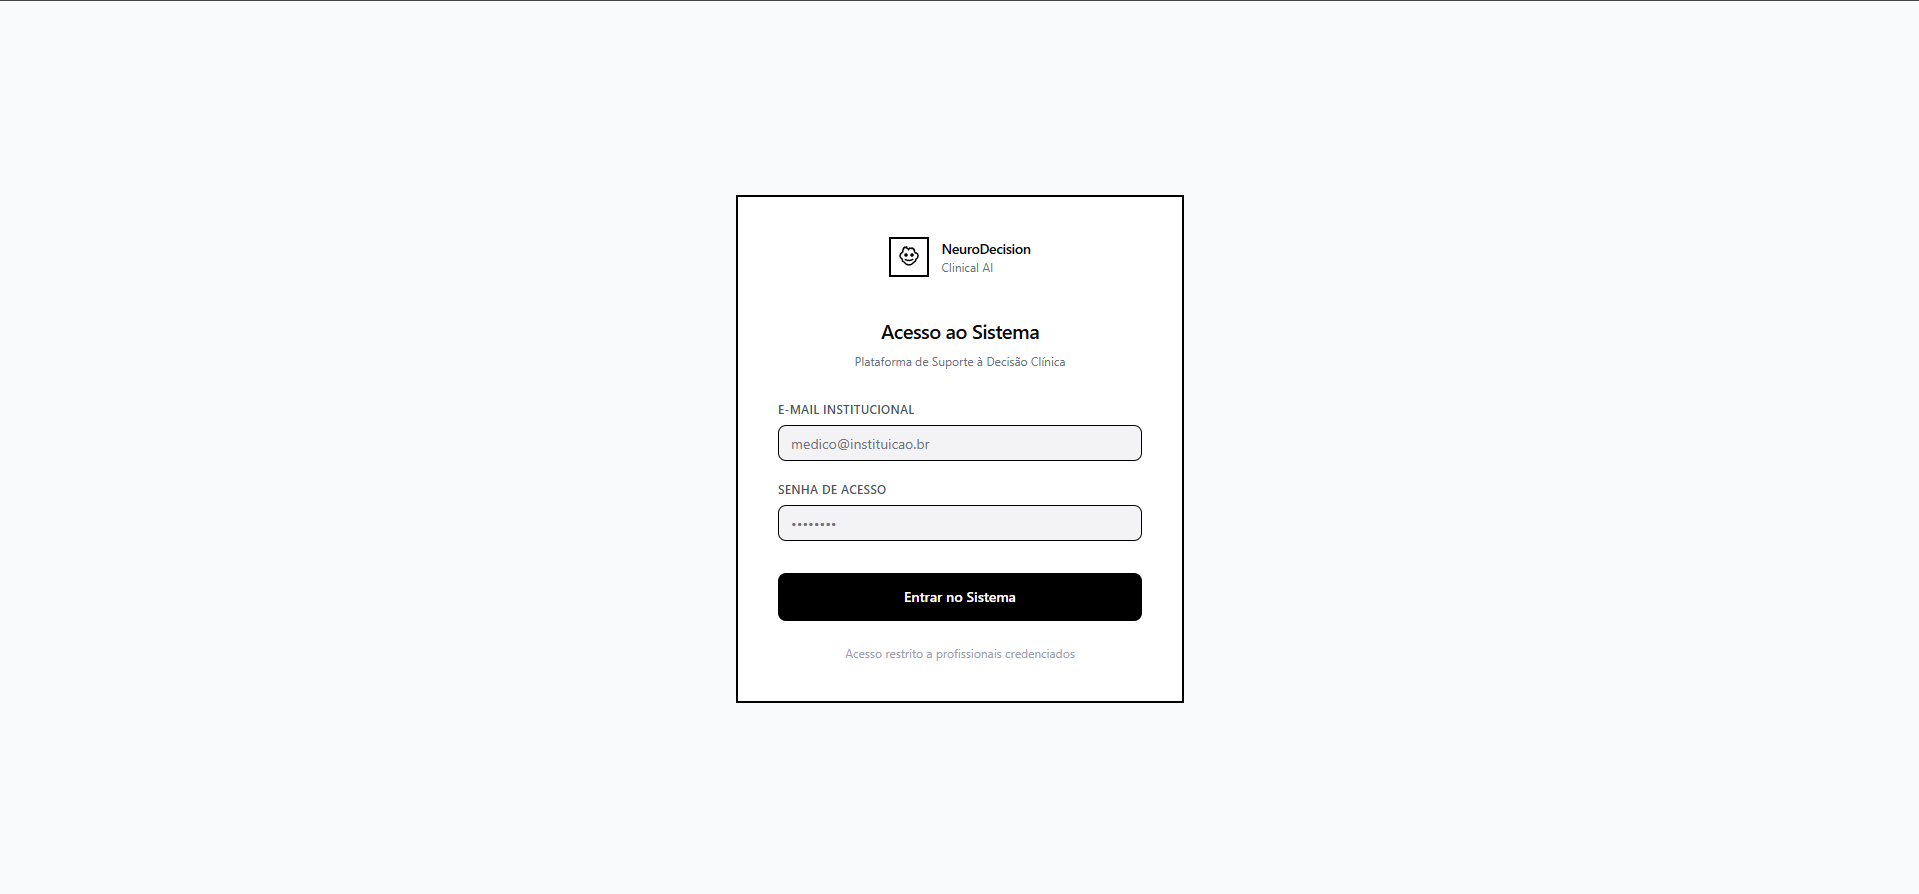
\includegraphics[width=13.60cm,height=0.72\textheight,keepaspectratio]{images/figura_05.png}\par
{\fontsize{10}{12}\selectfont Fonte: Elaborado pelo autor (2026).\par}
\end{figure}
A Figura 6 apresenta a interface de recuperação de senha. Na versão acadêmica, o fluxo é apenas simulado: a API devolve uma resposta neutra, mas não envia mensagem nem redefine credenciais. A recuperação operacional por e-mail permanece como trabalho futuro.

\begin{figure}[htbp]
\centering
\caption{Janela modal de recuperação de senha do sistema.}
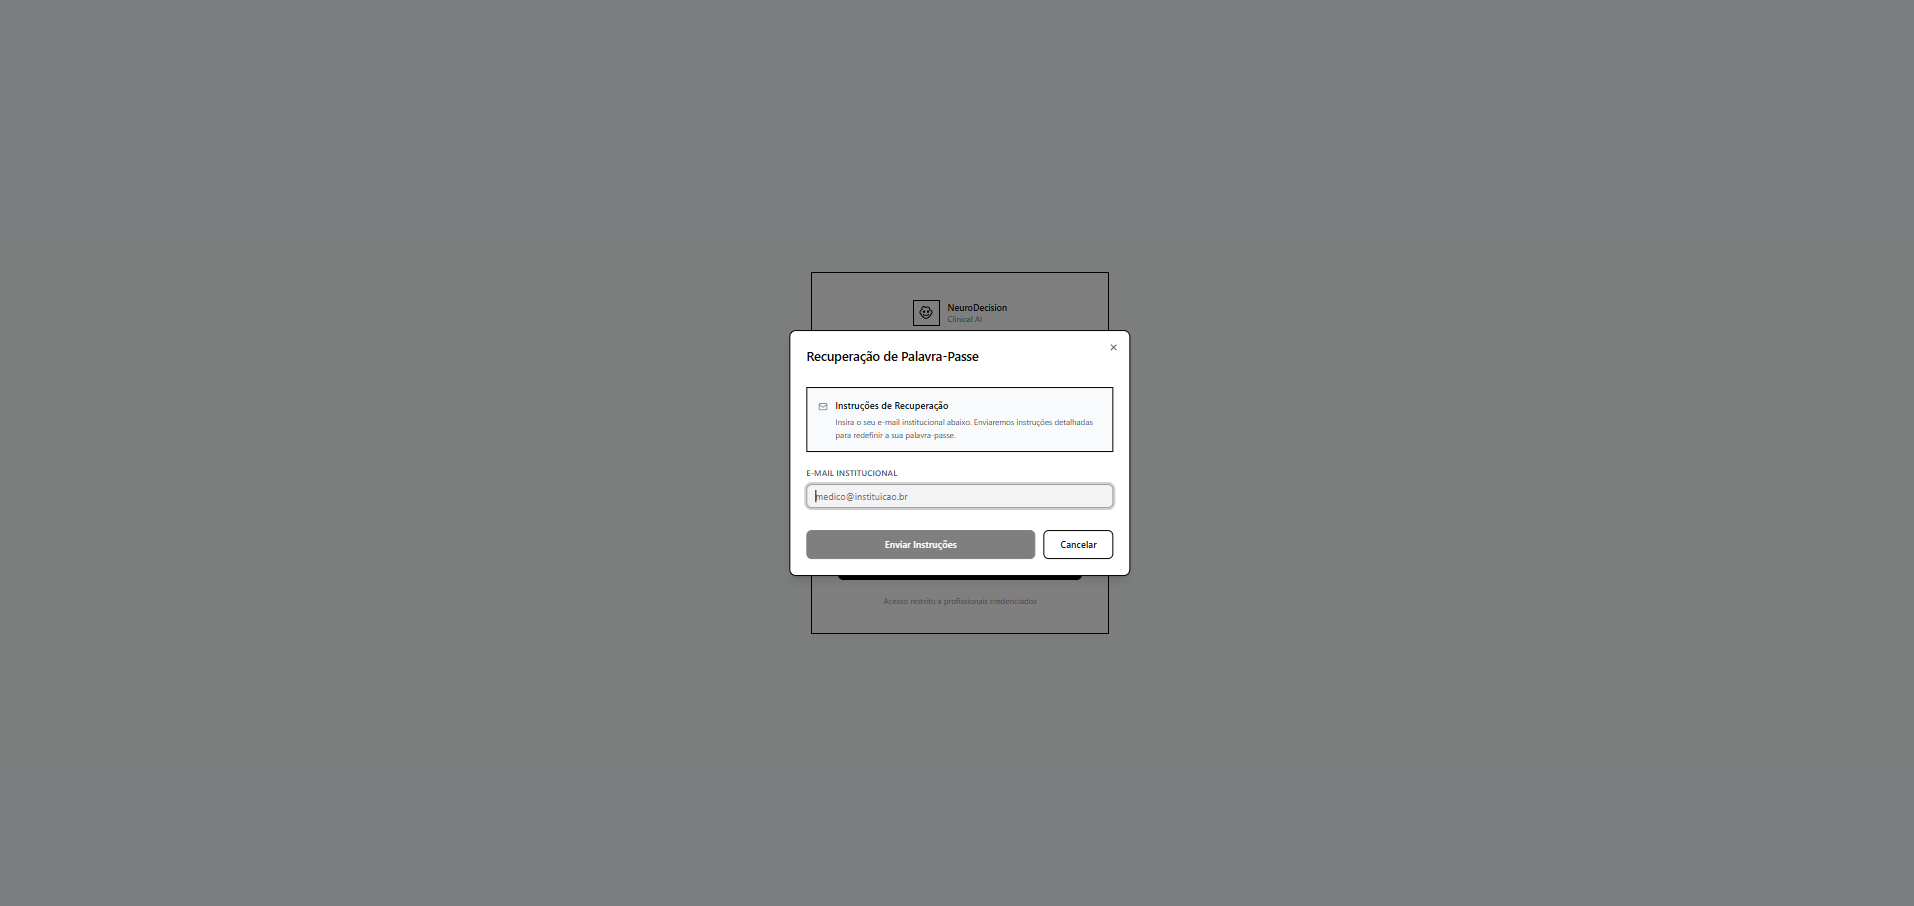
\includegraphics[width=13.60cm,height=0.72\textheight,keepaspectratio]{images/figura_04.png}\par
{\fontsize{10}{12}\selectfont Fonte: Elaborado pelo autor (2026).\par}
\end{figure}
A Figura 7 apresenta a tela inicial do sistema, também denominada Dashboard, que atua como o painel de controle principal para o especialista médico após a autenticação. A interface foi projetada para fornecer uma visão geral do ambiente clínico de forma clara e objetiva. O layout dispõe de um menu de navegação lateral e indicadores numéricos em destaque no topo, que resumem o volume de pacientes, exames em análise, laudos emitidos e um indicador de desempenho experimental do modelo preditivo. Esse indicador não representa a probabilidade de acerto de uma análise individual. O centro da tela é ocupado por uma tabela de atividades recentes para o acompanhamento de status dos exames, finalizando com atalhos de acesso rápido na seção inferior para otimizar o fluxo de trabalho diário do profissional.

\begin{figure}[htbp]
\centering
\caption{Tela inicial (Dashboard) e visão geral do sistema.}
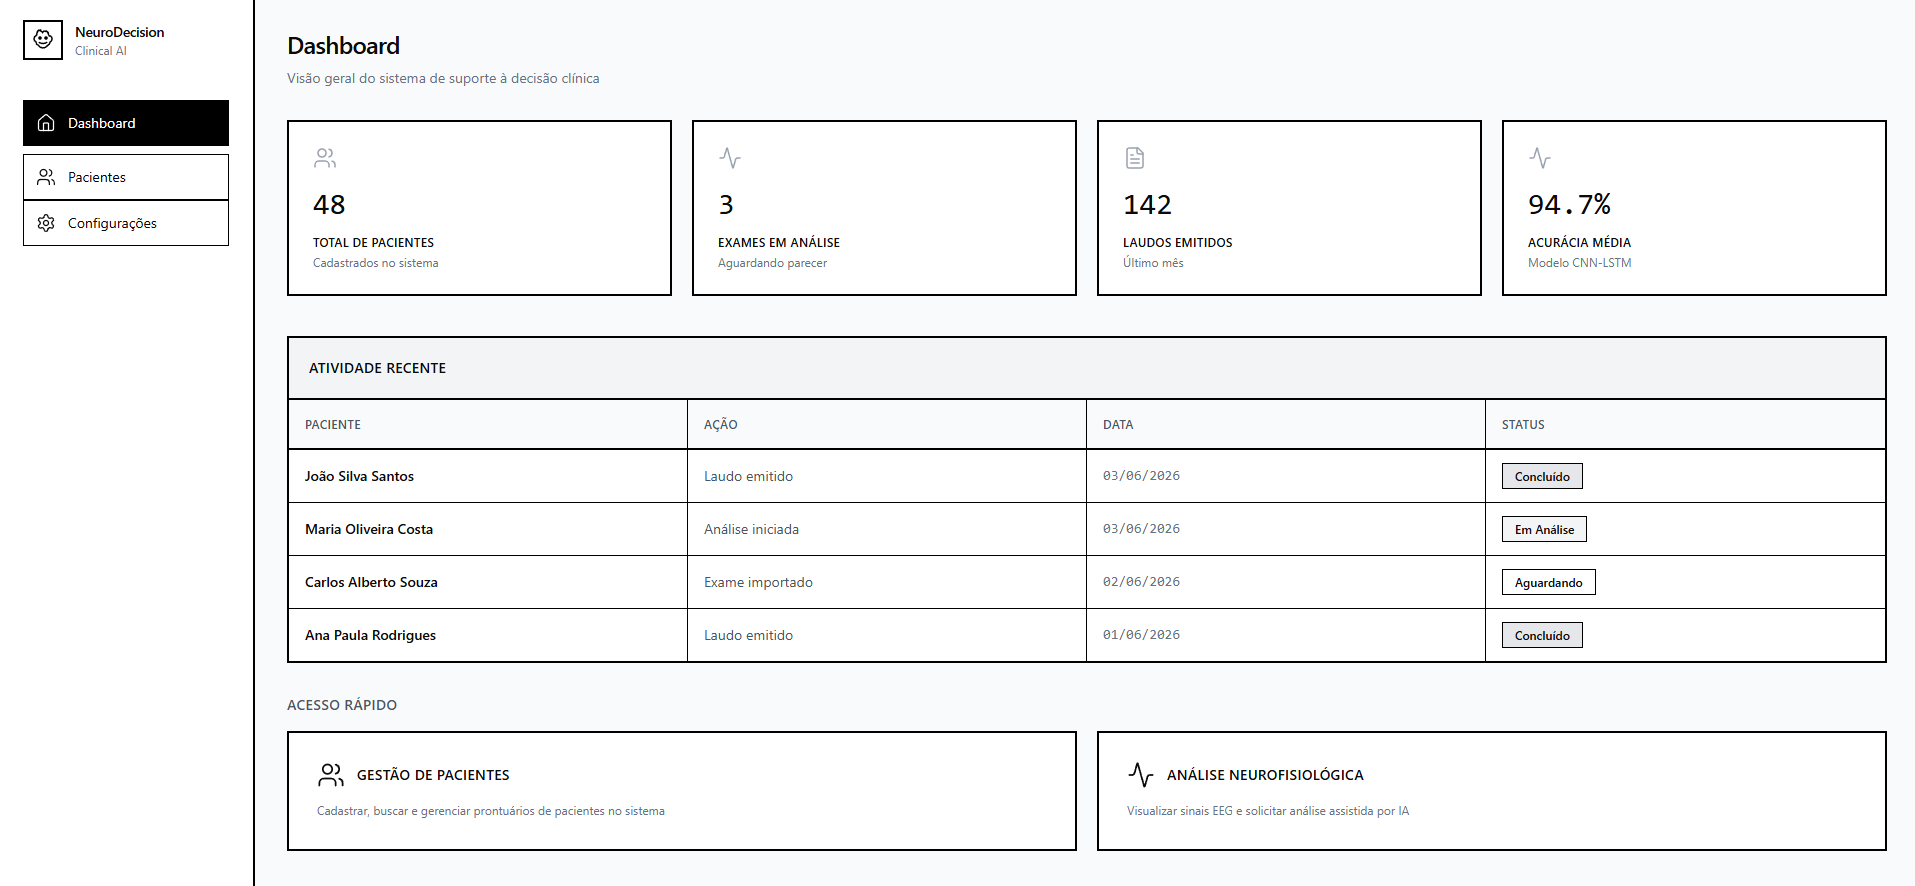
\includegraphics[width=13.60cm,height=0.72\textheight,keepaspectratio]{images/figura_07.png}\par
{\fontsize{10}{12}\selectfont Fonte: Elaborado pelo autor (2026).\par}
\end{figure}
A Figura 8 apresenta a interface de gestão de pacientes, dedicada ao registro e ao acompanhamento dos prontuários. A tela reúne pesquisa, cadastro, histórico de exames e situação do laudo, permitindo organizar o fluxo de trabalho do protótipo.

\begin{figure}[htbp]
\centering
\caption{Interface de gestão de pacientes e prontuários.}
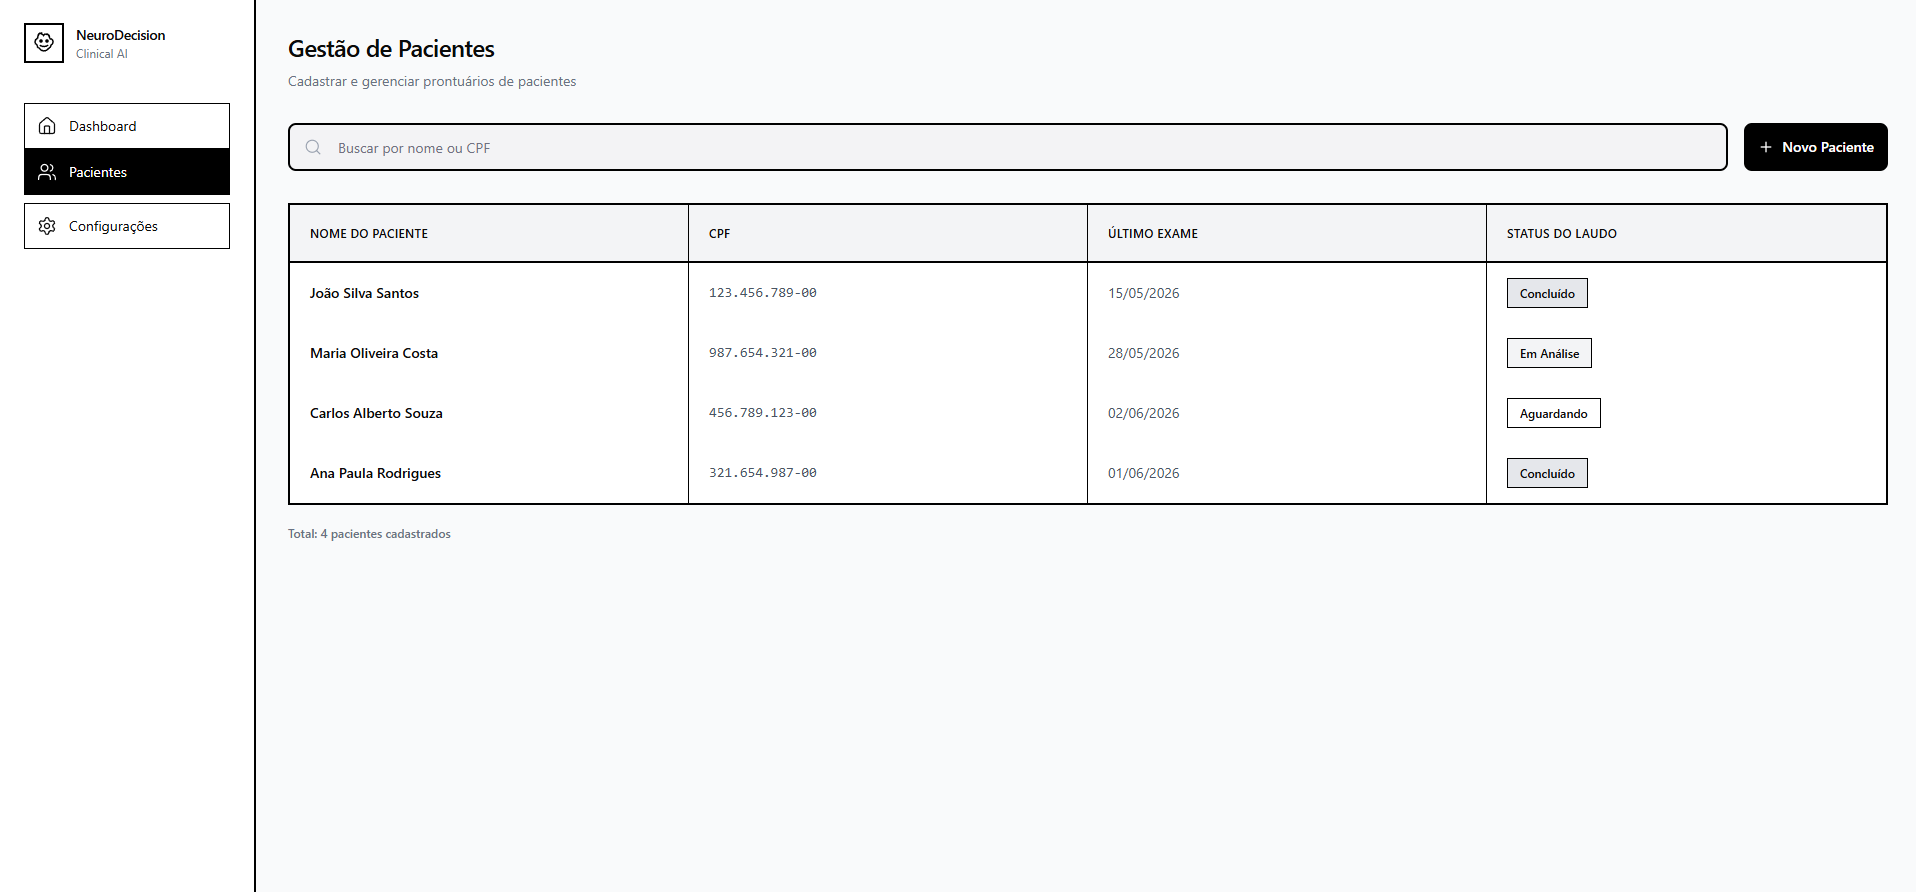
\includegraphics[width=13.60cm,height=0.72\textheight,keepaspectratio]{images/figura_06.png}\par
{\fontsize{10}{12}\selectfont Fonte: Elaborado pelo autor (2026).\par}
\end{figure}
A Figura 9 apresenta a interface de cadastro de um novo paciente, implementada no formato de janela sobreposta (modal). Acionada a partir da tela de gestão, a interface obscurece o plano de fundo para direcionar o foco do usuário ao formulário principal. O layout minimalista é composto por campos de entrada para os dados obrigatórios iniciais, como o nome completo e o CPF, além dos botões de confirmação ("Cadastrar Paciente") e cancelamento da ação. Esta abordagem de design permite a inserção ágil de informações no sistema sem a necessidade de redirecionamento de página, mantendo a fluidez do fluxo de trabalho clínico.

\begin{figure}[htbp]
\centering
\caption{Janela modal de cadastro de novo paciente.}
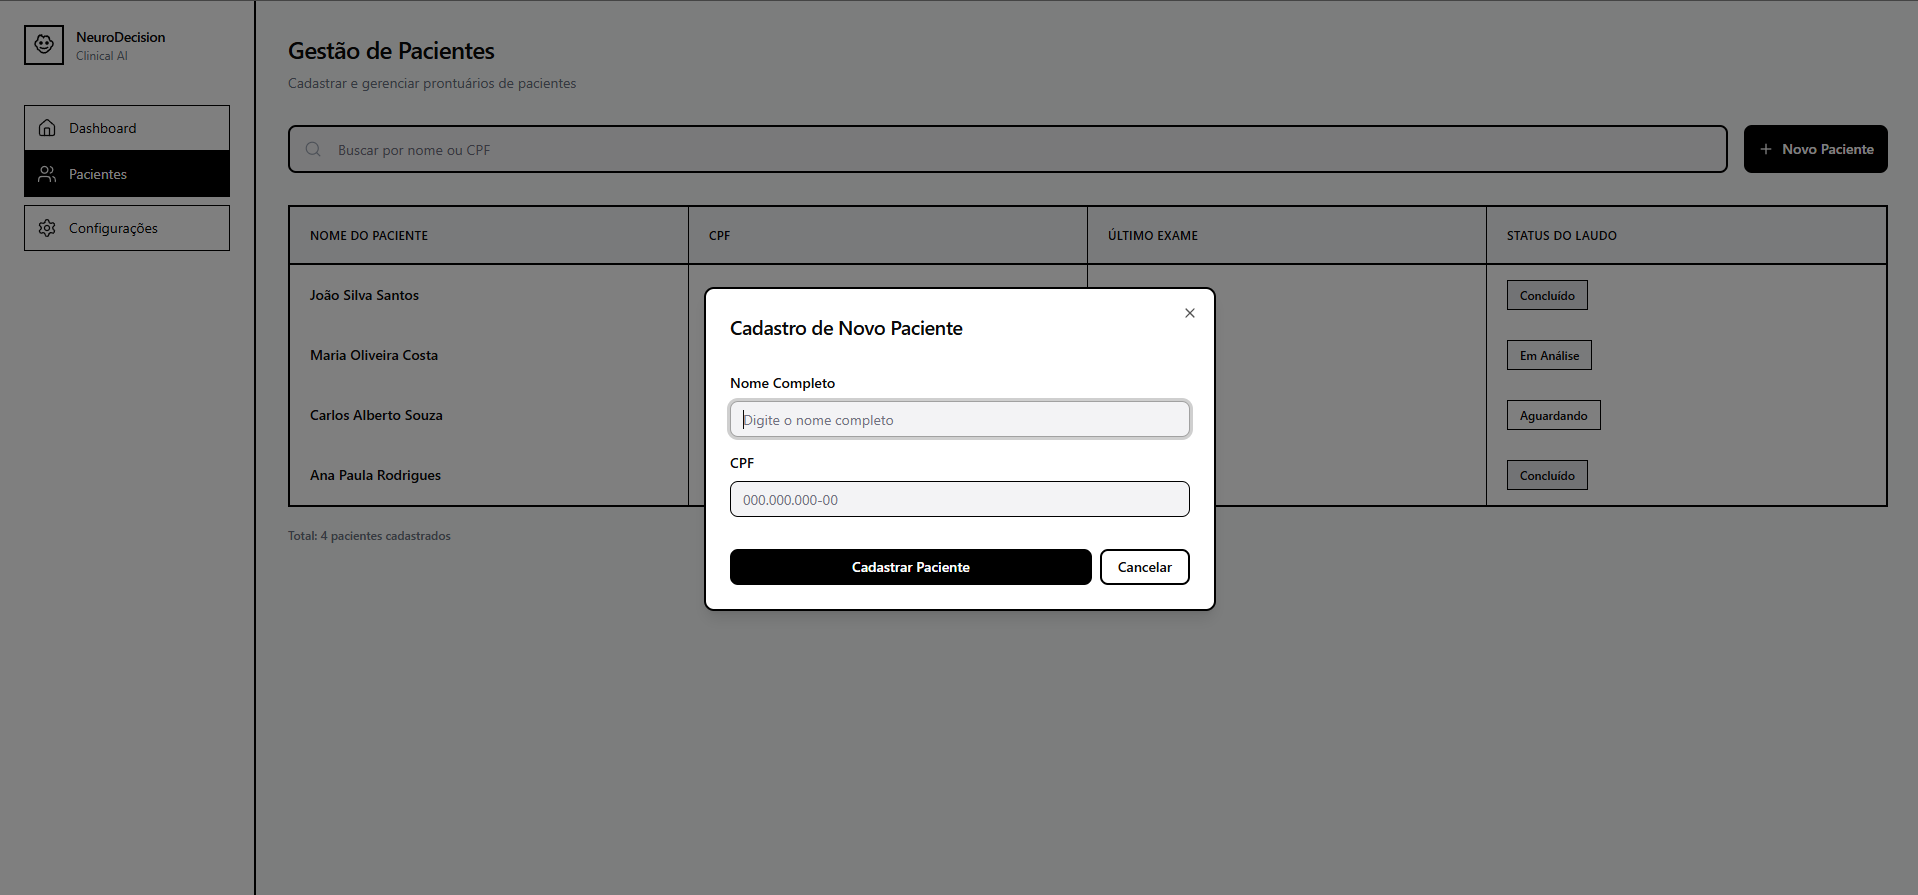
\includegraphics[width=13.60cm,height=0.72\textheight,keepaspectratio]{images/figura_09.png}\par
{\fontsize{10}{12}\selectfont Fonte: Elaborado pelo autor (2026).\par}
\end{figure}
A Figura 10 apresenta a interface central do sistema, dedicada à exploração visual dos sinais de Eletroencefalograma (EEG) e ao suporte à decisão clínica. O layout encontra-se estruturado em três colunas principais que refletem o fluxo de trabalho do neurologista. A seção lateral esquerda exibe os dados do paciente e possibilita a importação de novos exames no formato padrão EDF. A área central renderiza as séries temporais dos canais do EEG, oferecendo controles interativos de escala e amplitude, e prevê uma área de sobreposição gráfica onde atuará a Inteligência Artificial Explicável (mapas de calor gerados pelo método SHAP). Por fim, a coluna direita integra as ferramentas analíticas, disponibilizando a seleção dinâmica de eletrodos, o botão de acionamento do modelo preditivo (CNN-BiLSTM) e um editor de texto estruturado para a consolidação e emissão do laudo médico final.

\begin{figure}[htbp]
\centering
\caption{Interface central de visualização de EEG, análise de IA e laudo.}
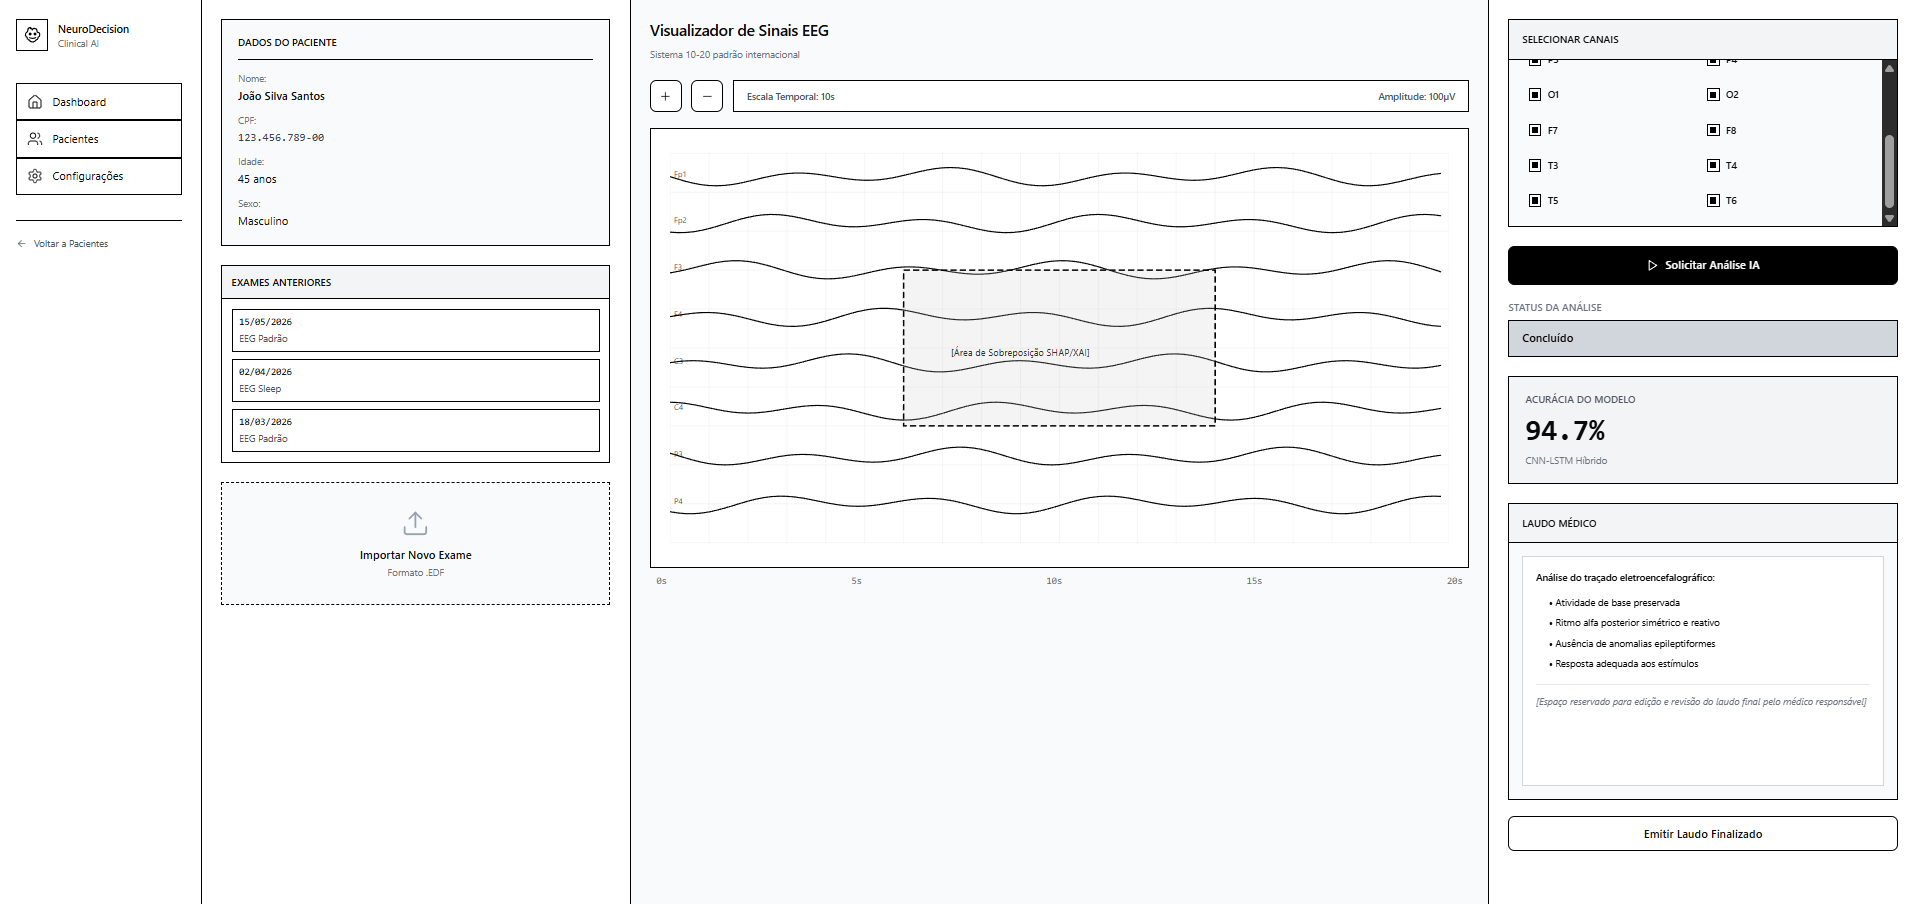
\includegraphics[width=13.60cm,height=0.72\textheight,keepaspectratio]{images/figura_08.png}\par
{\fontsize{10}{12}\selectfont Fonte: Elaborado pelo autor (2026).\par}
\end{figure}
A Figura 11 apresenta a tela de configurações, com dados profissionais, montagem padrão de canais, limiar de confiança e controle de exibição do SHAP. Essas preferências de interface não substituem a calibração científica do modelo.

\begin{figure}[htbp]
\centering
\caption{Interface de configurações do sistema e preferências de análise.}
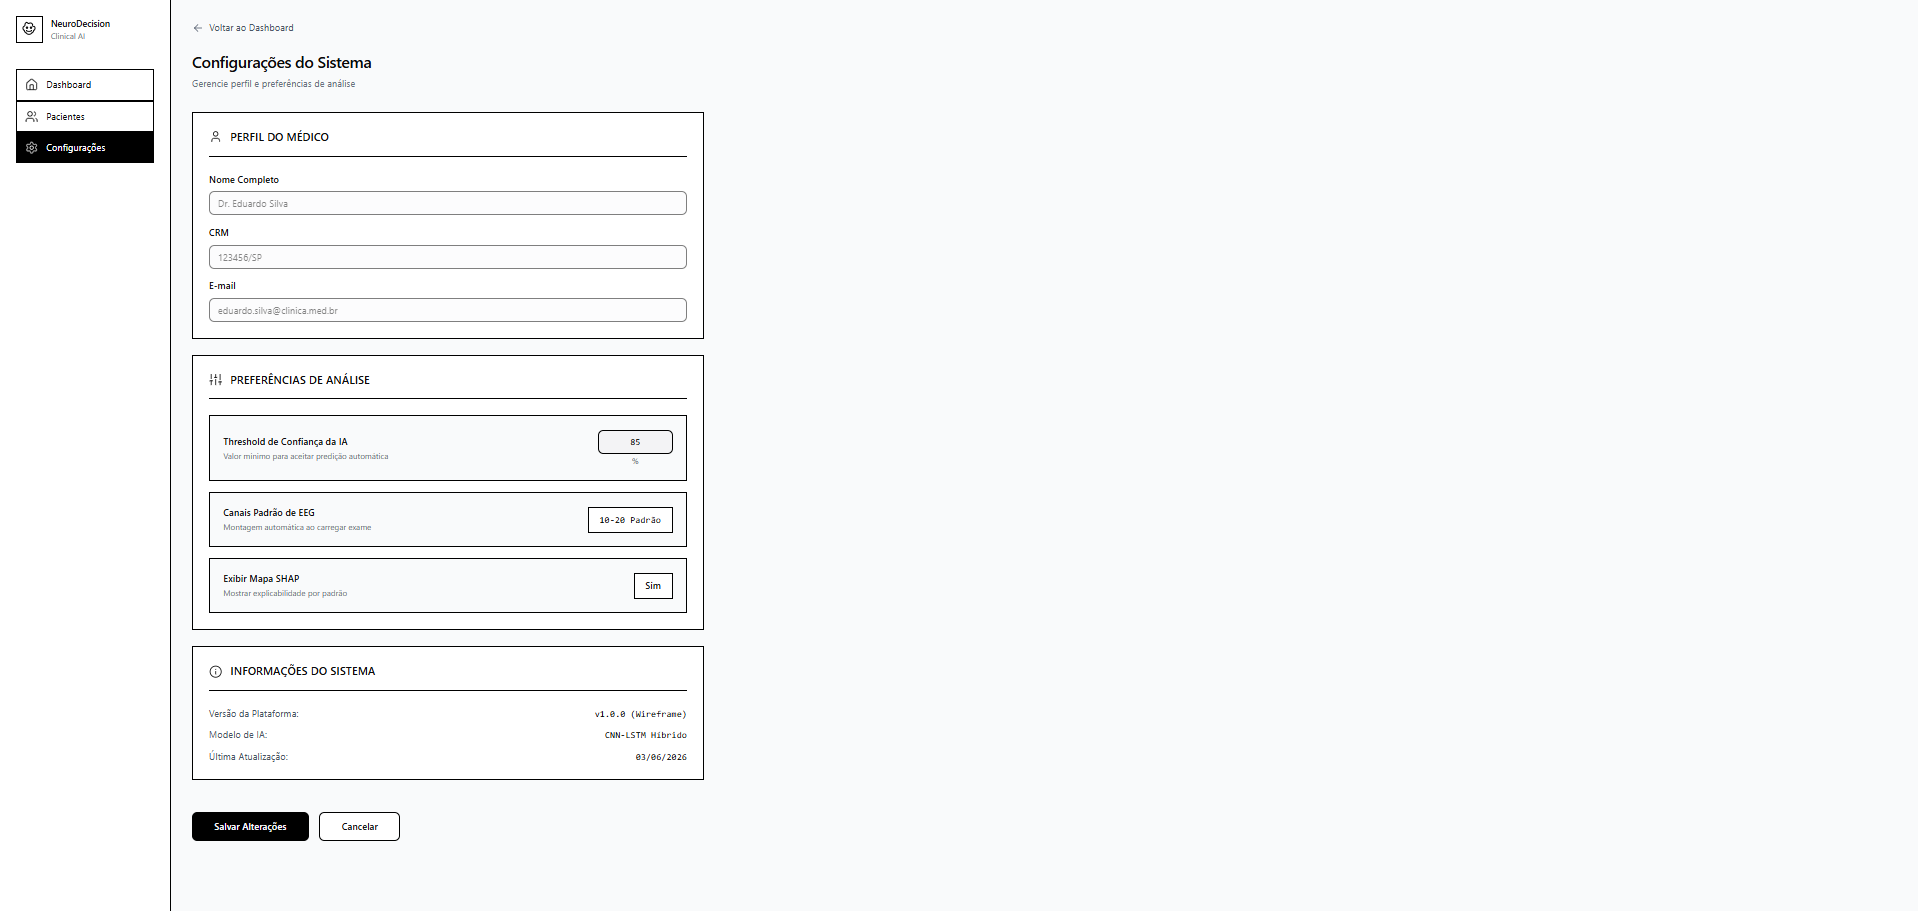
\includegraphics[width=13.60cm,height=0.72\textheight,keepaspectratio]{images/figura_10.png}\par
{\fontsize{10}{12}\selectfont Fonte: Elaborado pelo autor (2026).\par}
\end{figure}
A partir da concepção dessas interfaces de baixa fidelidade, estabeleceram-se as diretrizes visuais e funcionais necessárias para guiar a etapa de codificação do frontend em React.js e sua integração com a API FastAPI, cujas telas reais implementadas são apresentadas na seção de resultados.

\chapter{RESULTADOS}
\Needspace{12\baselineskip}\section{Interface implementada}
As Figuras 12 a 16 documentam a interface implementada no ambiente local: painel principal, gestão de pacientes, configurações, análise multicanal com sobreposição SHAP e redação do laudo médico.

A Figura 12 apresenta o painel principal (Visão geral) da versão implementada após a autenticação médica. A interface exibe a identificação do profissional logado na barra lateral e organiza no topo os indicadores de pacientes cadastrados, exames pendentes e laudos emitidos, além de disponibilizar atalhos de acesso rápido para abertura de prontuários e ajuste das preferências de análise.

\begin{figure}[htbp]
\centering
\caption{Painel principal da versão implementada.}
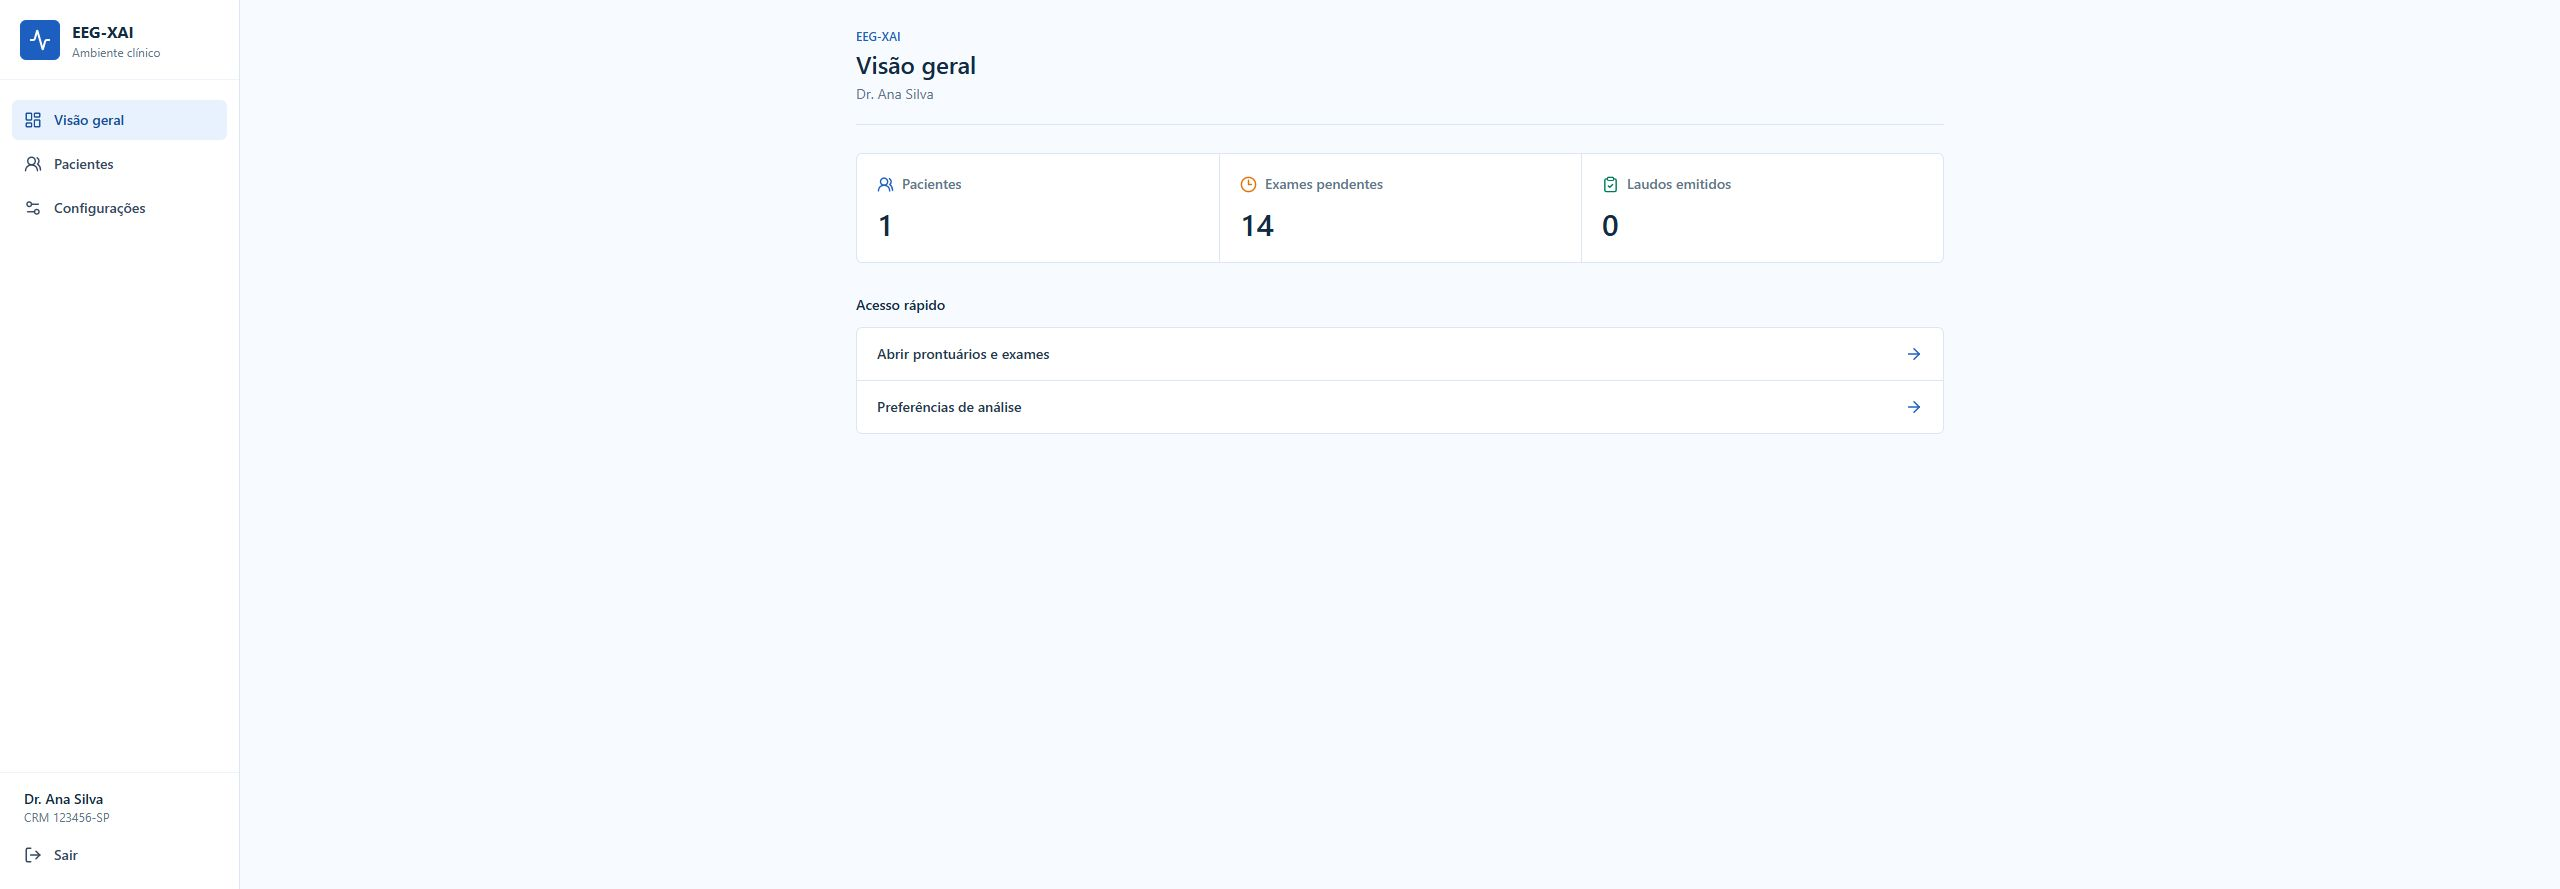
\includegraphics[width=13.60cm,height=0.72\textheight,keepaspectratio]{images/figura_12.png}\par
{\fontsize{10}{12}\selectfont Fonte: Elaborado pelo autor (2026).\par}
\end{figure}
A Figura 13 ilustra a tela implementada para a gestão de pacientes. O módulo disponibiliza um campo de busca filtrada por nome ou CPF, o botão de ação para cadastro de novos registros e a listagem tabular dos pacientes ativos, integrando botões em cada linha para editar dados, excluir registros ou encaminhar diretamente o prontuário para a importação de um novo exame de EEG.

\begin{figure}[htbp]
\centering
\caption{Gestão de pacientes da versão implementada.}
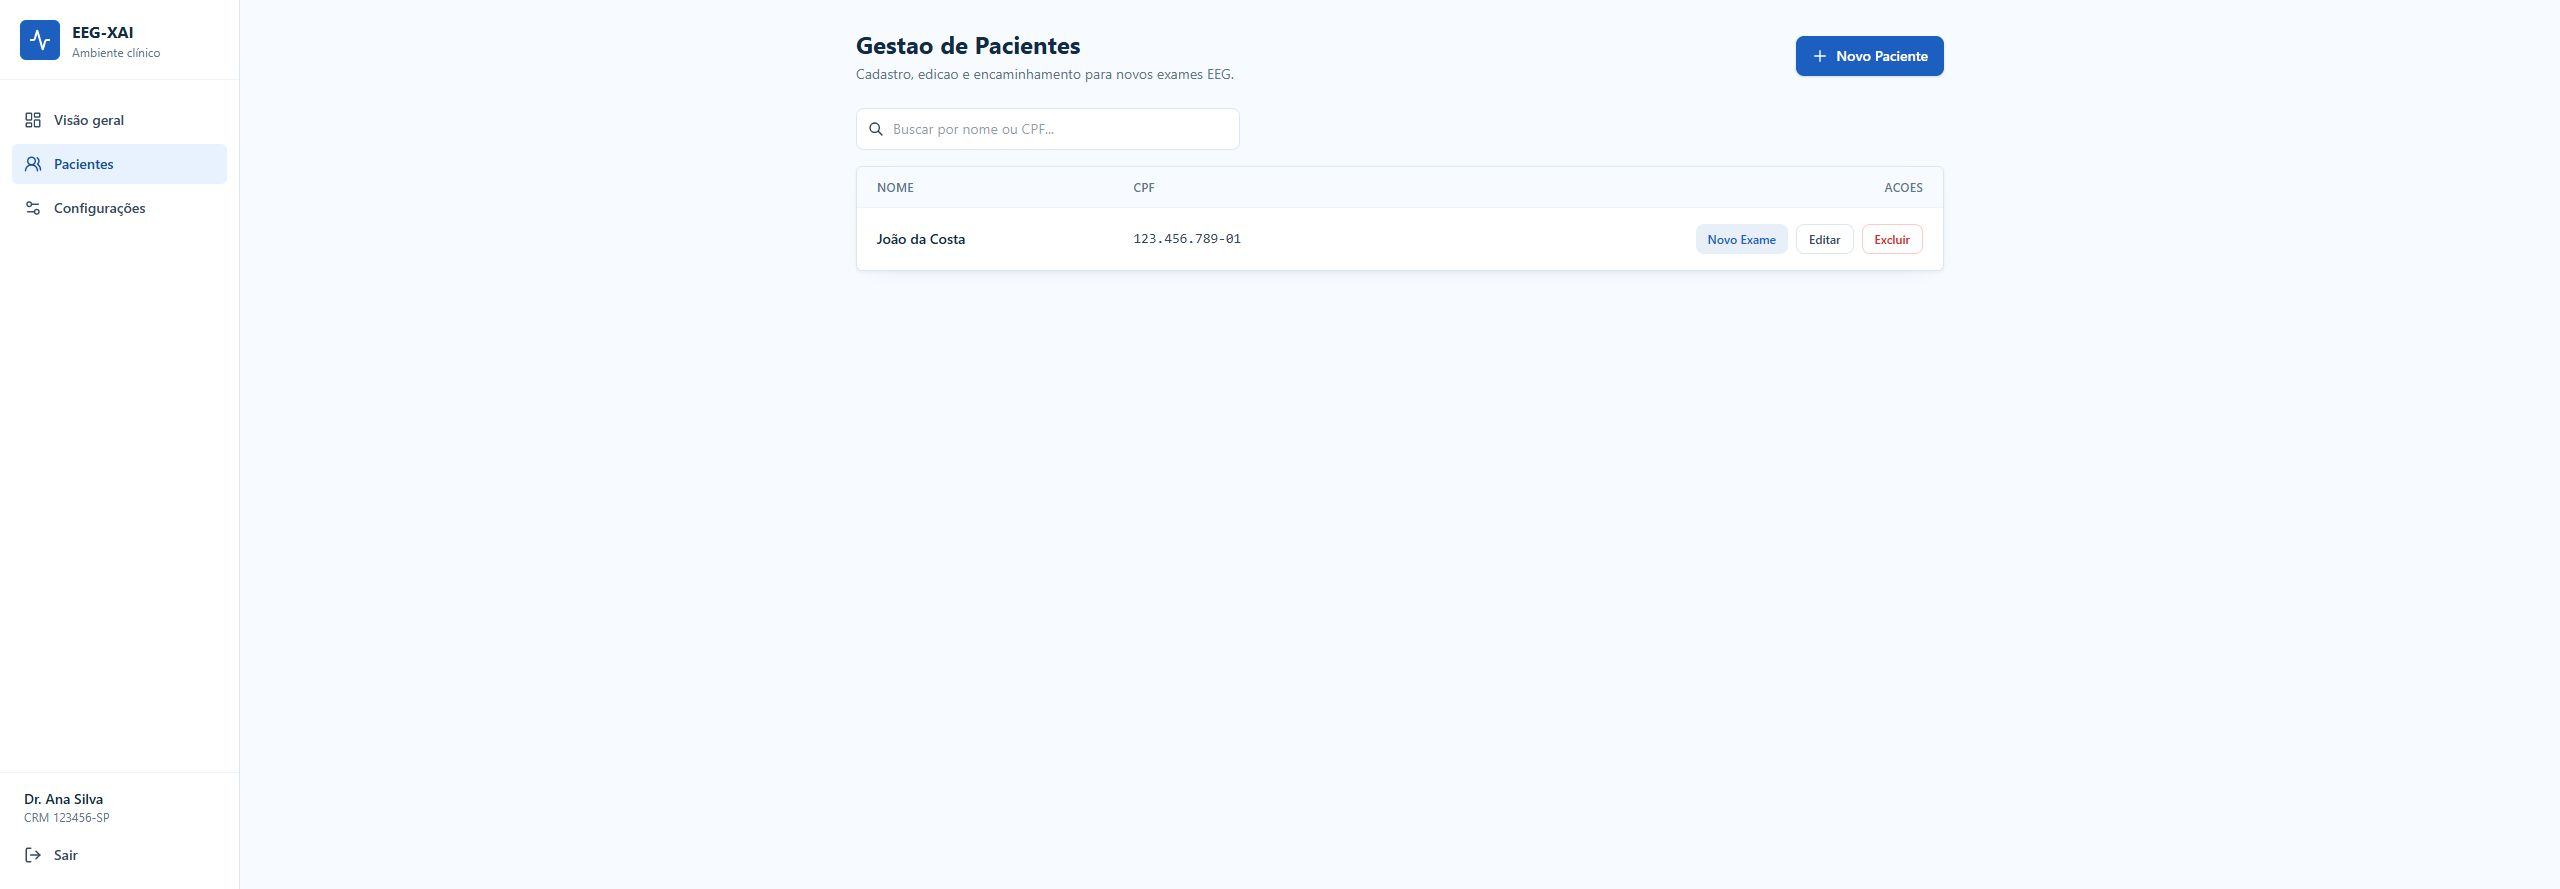
\includegraphics[width=13.60cm,height=0.72\textheight,keepaspectratio]{images/figura_13.png}\par
{\fontsize{10}{12}\selectfont Fonte: Elaborado pelo autor (2026).\par}
\end{figure}
A Figura 14 apresenta a interface implementada para as configurações do sistema. Nela, o especialista gerencia seus dados de perfil (nome, CRM e e-mail), seleciona os canais preferenciais da montagem longitudinal bipolar como referência padrão para novas análises e pode habilitar ou desabilitar a exibição dos mapas SHAP. A preferência ajustável de limiar (threshold) aplica-se somente ao modelo legado; na CNN-BiLSTM v43, a decisão sequencial segue os parâmetros definidos no artefato científico de calibração, independentemente do valor configurado no perfil médico.

\begin{figure}[htbp]
\centering
\caption{Configurações do perfil, montagem, limiar e SHAP.}
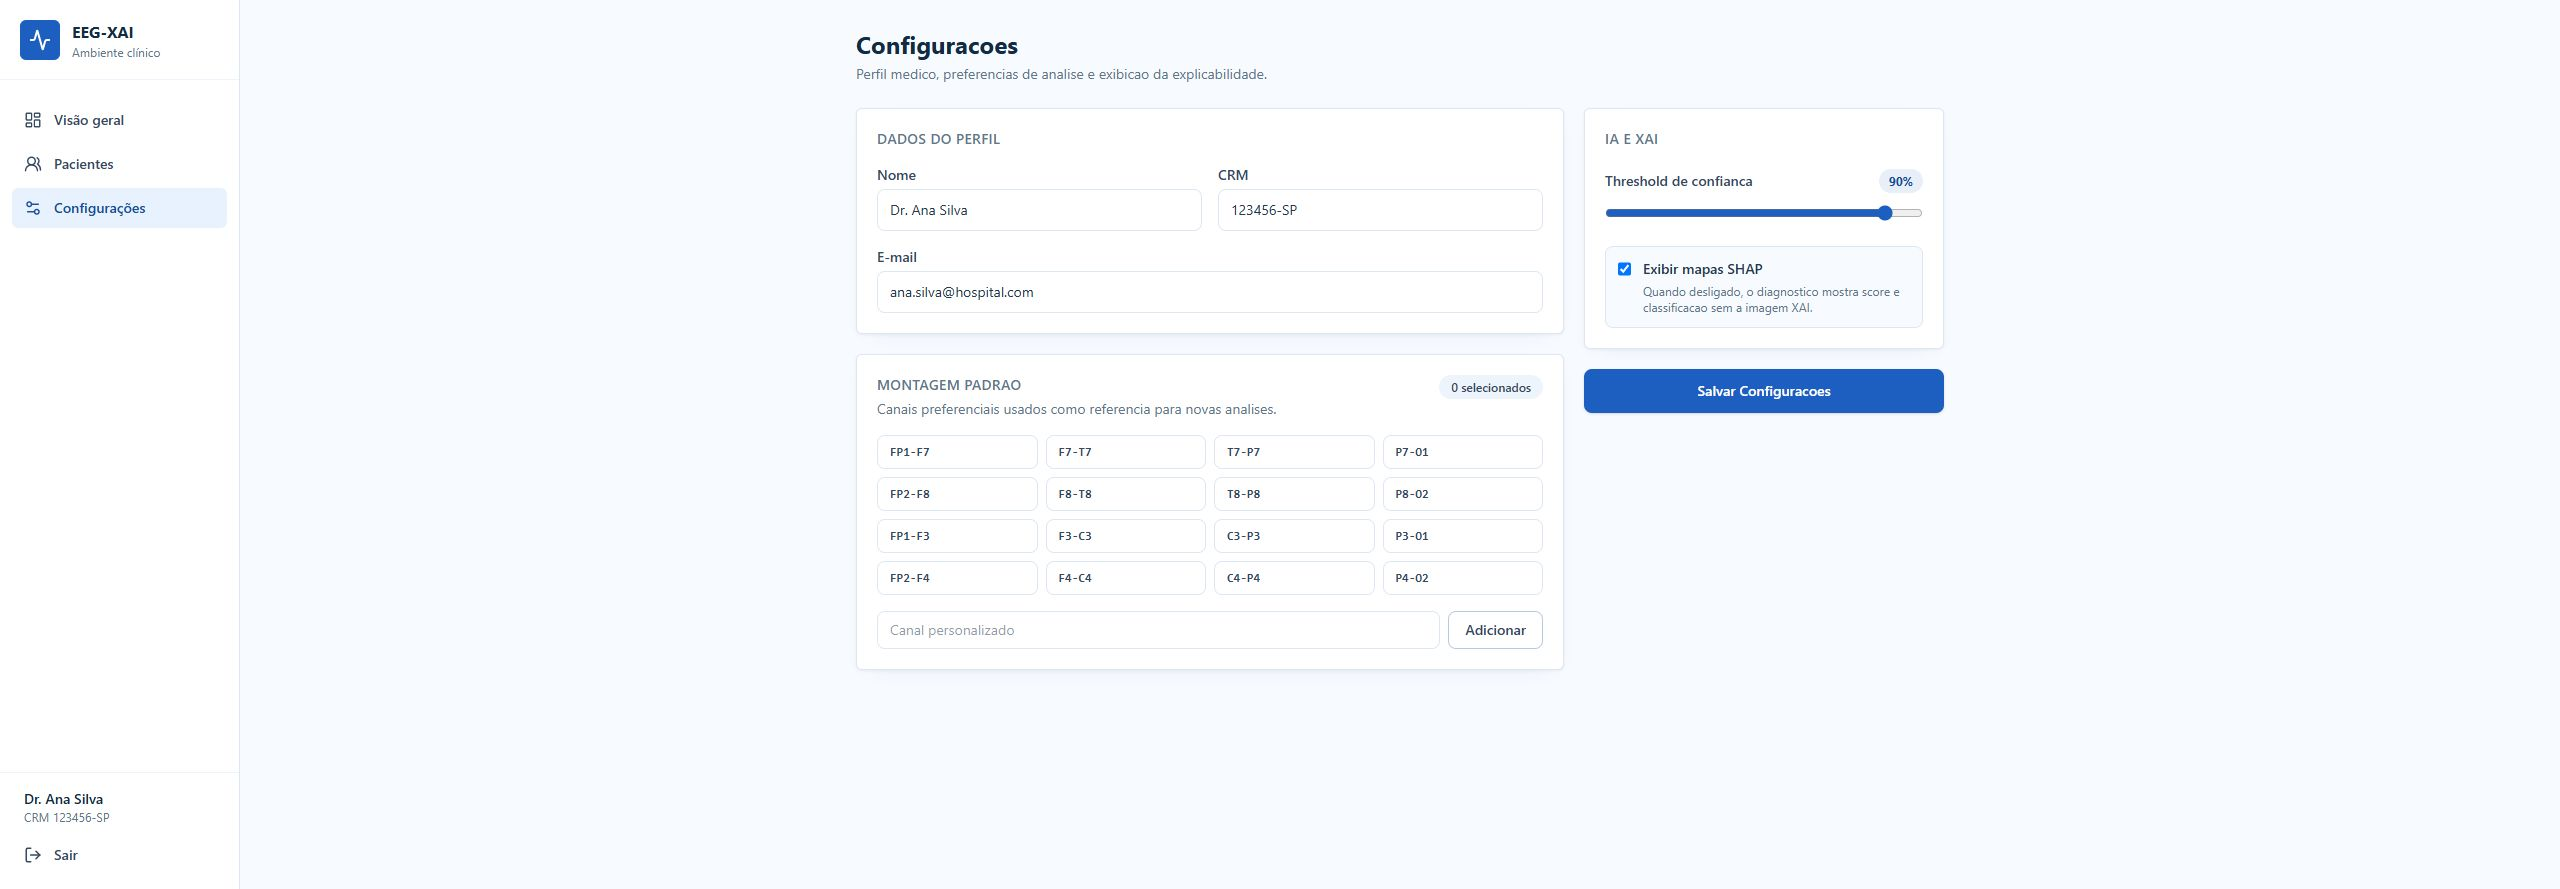
\includegraphics[width=13.60cm,height=0.72\textheight,keepaspectratio]{images/figura_14.png}\par
{\fontsize{10}{12}\selectfont Fonte: Elaborado pelo autor (2026).\par}
\end{figure}
A Figura 15 demonstra a tela central de visualização multicanal de EEG operando sobre um registro real de 23 canais. Na coluna esquerda, a interface reúne os dados cadastrais e o histórico do paciente, juntamente com a área de upload para arquivos no formato .edf. No painel central, o traçado das séries temporais é renderizado com controles superiores de navegação e zoom; nele, a faixa laranja delimita o trecho suspeito e a intensidade vermelha representa a contribuição positiva do Gradient SHAP. A projeção está associada às janelas de características da sequência de pico; portanto, não corresponde a uma atribuição para cada amostra bruta do sinal. Na coluna direita, na aba de Análise, são exibidos o seletor de canais, o status do motor de IA e o Escore de Suspeita acompanhado da observação explícita de que a métrica atua como apoio, e não como diagnóstico.

\begin{figure}[htbp]
\centering
\caption{Visualização multicanal com trecho suspeito e SHAP sobreposto por canal e tempo.}
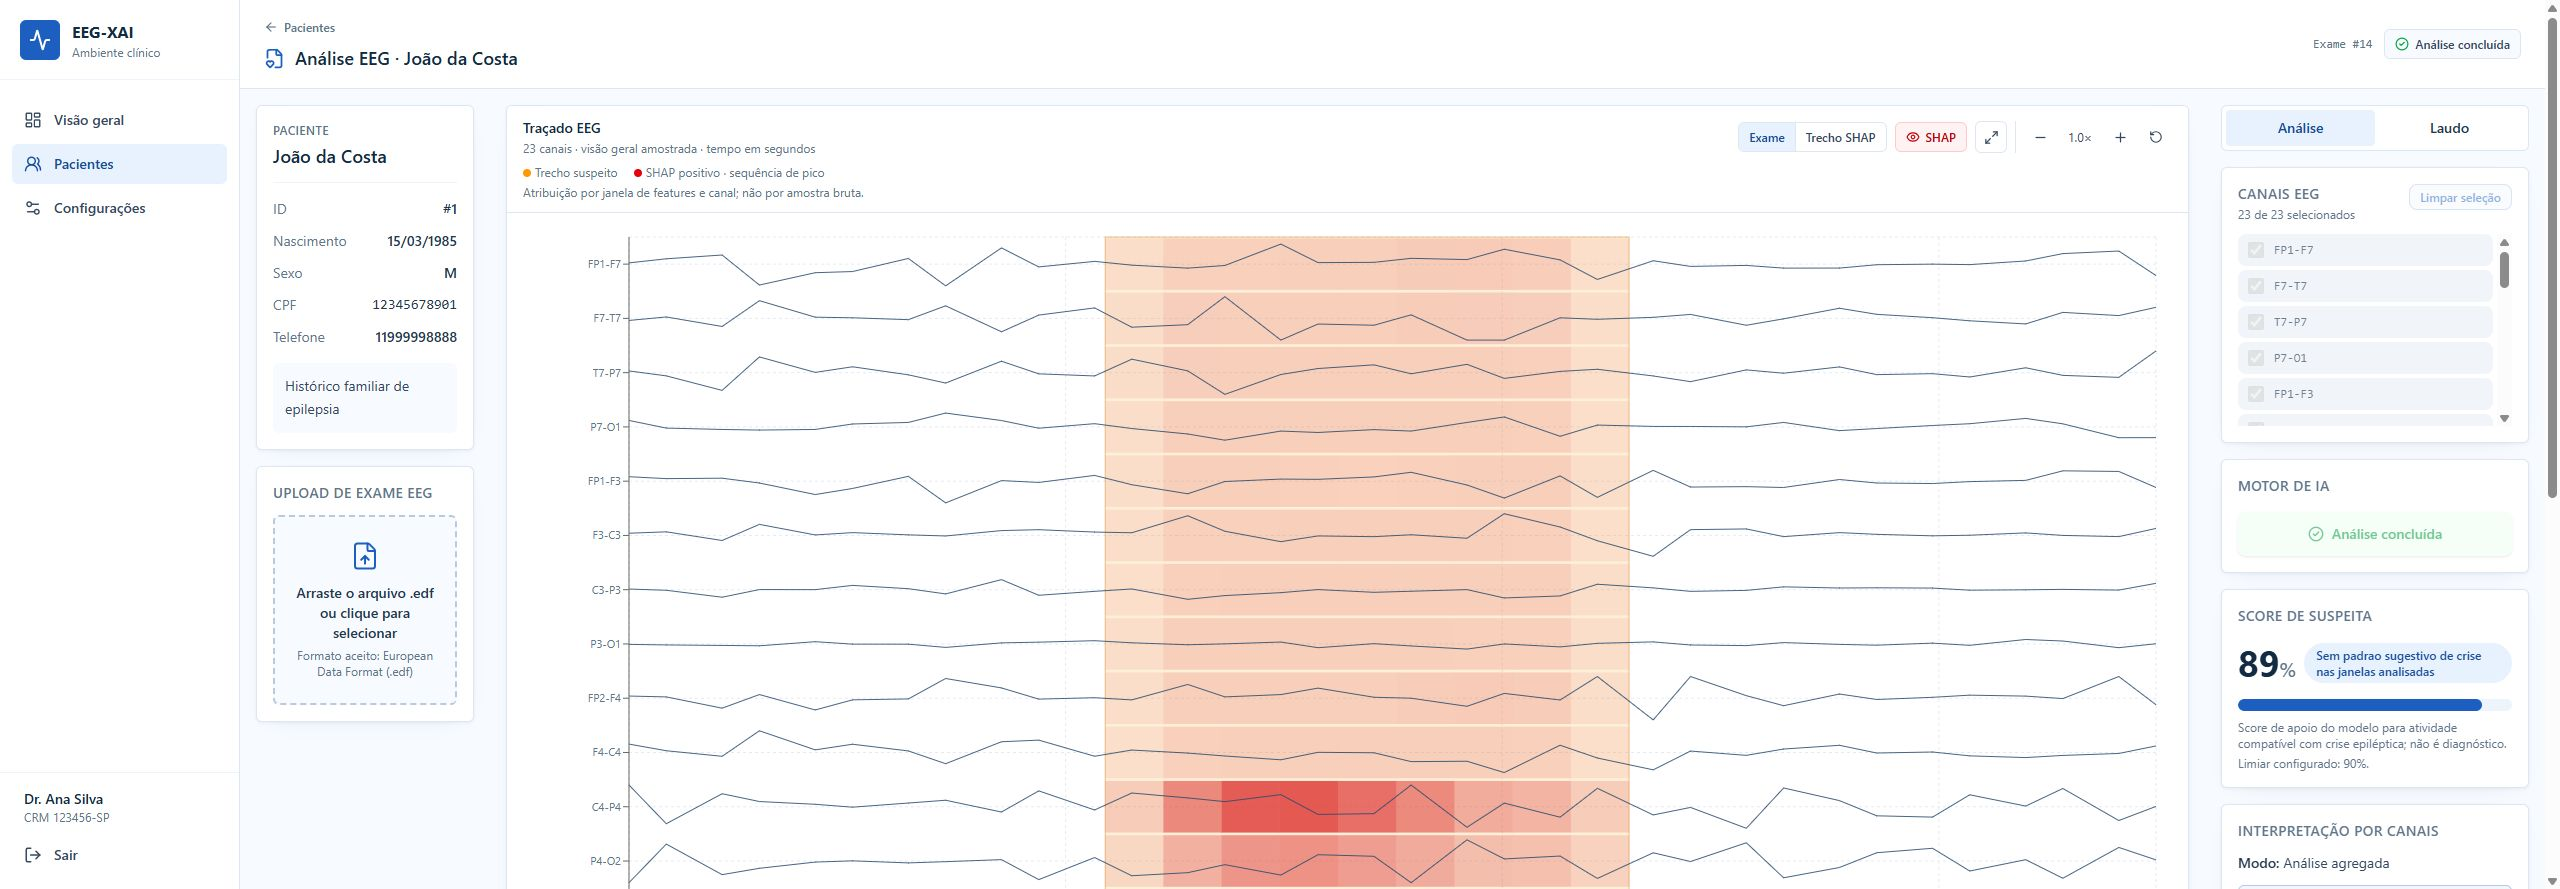
\includegraphics[width=13.60cm,height=0.72\textheight,keepaspectratio]{images/figura_15.png}\par
{\fontsize{10}{12}\selectfont Fonte: Elaborado pelo autor (2026).\par}
\end{figure}
Por fim, a Figura 16 apresenta a área de emissão do parecer médico na coluna lateral direita (aba Laudo), mantendo o traçado de EEG e a sobreposição do SHAP visíveis ao centro para inspeção simultânea. O componente disponibiliza um campo textual para que o especialista descreva a interpretação clínica do exame correlacionando a saída da IA com o quadro do paciente, finalizando o fluxo por meio do botão de emissão do laudo.

\begin{figure}[htbp]
\centering
\caption{Área de emissão do parecer médico após a análise computacional.}
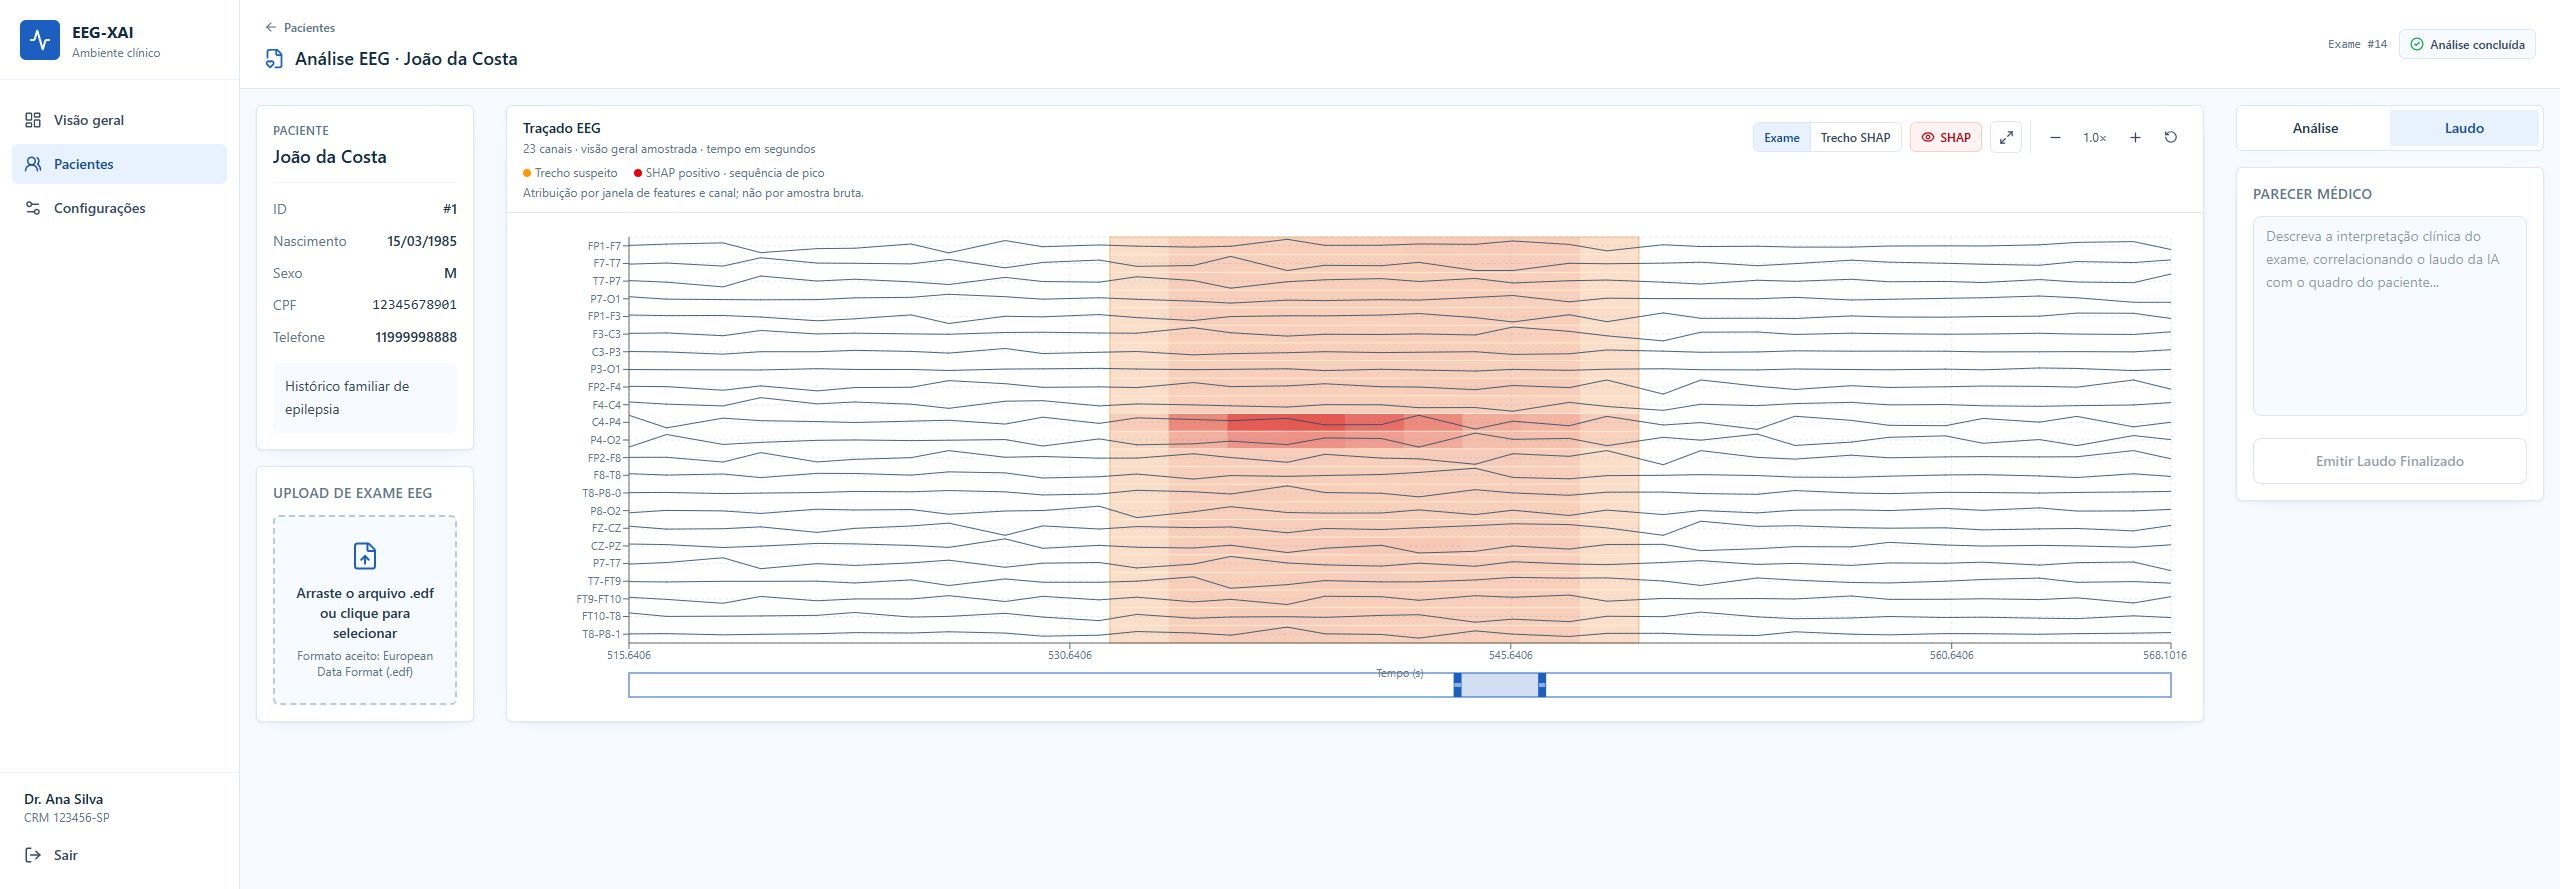
\includegraphics[width=13.60cm,height=0.72\textheight,keepaspectratio]{images/figura_16.png}\par
{\fontsize{10}{12}\selectfont Fonte: Elaborado pelo autor (2026).\par}
\end{figure}
\Needspace{12\baselineskip}\section{Protocolo experimental}
O modelo final selecionado foi a versão v43 com seed 42. A arquitetura CNN-BiLSTM utiliza fusão tardia de 23 canais e 15 características tempo-frequência por canal, entre elas a entropia espectral. Não utiliza a característica histórica de Entropia de Shannon nem medidas de Dinâmica Simbólica. As janelas têm 4 segundos, passo de 2 segundos e sequências de 8 passos. O treinamento utilizou 77 EDFs de 17 grupos identificados na base; a calibração reuniu 13 EDFs de chb16, chb19, chb20 e chb24, separados antes do janelamento.

O ponto operacional foi definido exclusivamente na calibração, com limiar de 0,60, duração mínima de 18 segundos e fechamento de lacunas de 8 segundos. A seleção do checkpoint priorizou desempenho por evento sob limite de falsos alarmes por hora. O conjunto chb09, chb15 e chb18 foi mantido separado no experimento final, mas já havia sido consultado durante o desenvolvimento; por isso, seus resultados são classificados como avaliação histórica, e não como teste final intocado. O limiar é aplicado aos escores temporais de suspeita e não significa que o modelo tenha precisão de 60\% nem equivale a uma probabilidade clínica calibrada.

O Quadro a seguir consolida a receita experimental da versão integrada à aplicação. Além da normalização robusta por EDF, baseada em mediana e intervalo interquartil com limitação de valores extremos, foi aplicado o escalonador ajustado exclusivamente sobre o conjunto de treino. A BCE recebeu pesos por amostra derivados do balanceamento de classes e da amostragem por evento, evitando que crises longas dominassem apenas por produzirem mais janelas.

\FloatBarrier\Needspace{9\baselineskip}
\captionof{table}{Configuração reproduzível do modelo final v43, seed 42}\nopagebreak[4]
\begingroup
\fontsize{10}{12}\selectfont
\setlength{\tabcolsep}{4pt}
\renewcommand{\arraystretch}{1.15}
\addtocounter{table}{-1}
\begin{longtable}{|>{\raggedright\arraybackslash}p{0.30\textwidth}|>{\raggedright\arraybackslash}p{0.63\textwidth}|}
\hline
\textbf{Elemento} & \textbf{Configuração} \\ \hline
\endfirsthead
\hline
\textbf{Elemento} & \textbf{Configuração} \\ \hline
\endhead
Entrada & 23 canais bipolares; 15 características por canal; 345 valores por janela. \\ \hline
Características & Potência absoluta e relativa nas bandas delta (0,5--4 Hz), theta (4--8 Hz), alpha (8--13 Hz), beta (13--30 Hz) e gamma (30--45 Hz); frequência dominante; centroide espectral; entropia espectral; razões theta/alpha e beta/alpha. \\ \hline
Organização temporal & Janelas de 4 s, passo de 2 s, sequência de 8 passos, stride de sequência 2 e rótulo ictal da janela com sobreposição mínima de 50\% em relação à anotação. \\ \hline
Normalização & Normalização robusta por EDF, seguida de scaler ajustado somente no treino; canais ausentes mantidos mascarados após o escalonamento. \\ \hline
Arquitetura & Projeção temporal compartilhada por canal com duas convoluções 2D de 16 filtros, fusão tardia por Conv1D de 64 filtros, Conv1D temporal de 64 filtros, BiLSTM com 48 unidades por direção e saída sigmoide por passo. \\ \hline
Regularização & L2 de $10^{-4}$ nas convoluções por canal; normalização por camada; dropout de 0,20, 0,25 e 0,20. \\ \hline
Otimização & Entropia cruzada binária ponderada, Adam com taxa de aprendizado 0,001, lote 32, limite de 20 épocas e amostragem balanceada por evento. \\ \hline
Seleção & Checkpoint por recall de evento sob FA/h $\leq 0{,}75$, com critério de desempate orientado à localização; melhor época: 14; seed: 42. \\ \hline
Volume efetivo & 77 EDFs de treino, 4.648 sequências de treino, sendo 952 positivas; 13 EDFs de calibração, 11.587 sequências, sendo 153 positivas. \\ \hline
Capacidade & 84.081 parâmetros treináveis. \\ \hline
Pós-processamento & Limiar 0,60, duração mínima 18 s e fechamento de lacunas de até 8 s, definidos somente na calibração. \\ \hline
\end{longtable}
\endgroup
\nopagebreak[4]{\centering\fontsize{10}{12}\selectfont Fonte: Elaborado pelo autor a partir dos artefatos da v43 (2026).\par}

A base Bonn, prevista no planejamento do TCC I, não foi combinada à avaliação final. Seus segmentos curtos e previamente selecionados não preservam o mesmo protocolo de registros contínuos multicanais com início e término de crises do CHB-MIT. A mistura direta dificultaria interpretar métricas de localização temporal e falsos alarmes por hora. Assim, os resultados apresentados nesta pesquisa referem-se ao CHB-MIT; Bonn permanece como referência do planejamento.

O processamento pode ser interpretado em três níveis. Primeiro, cada janela é convertida em características numéricas por canal. Em seguida, a CNN aprende combinações dessas características e a BiLSTM modela sua evolução dentro da sequência, produzindo oito escores temporais. Por fim, as saídas de sequências sobrepostas são agregadas e o pós-processamento forma intervalos para revisão. A saída sigmoide está entre zero e um, mas não foi demonstrado que ela represente uma probabilidade clínica calibrada. O uso de contexto bidirecional e de normalização por EDF caracteriza a análise de um registro disponível, sem demonstração de detecção em tempo real.

\begin{figure}[htbp]
\centering
\caption{Etapas da análise temporal na versão v43.}\label{fig:fluxo-v43}
\begin{minipage}{0.91\textwidth}
\centering\small
\fbox{\parbox{0.94\linewidth}{\centering EDF multicanal: janelas de 4 s, deslocadas a cada 2 s}}\par
$\downarrow$\par
\fbox{\parbox{0.94\linewidth}{\centering 23 canais $\times$ 15 características: 345 valores por janela\\Sequências de 8 passos}}\par
$\downarrow$\par
\fbox{\parbox{0.94\linewidth}{\centering Convoluções temporais por canal $\rightarrow$ fusão tardia\\Convolução temporal $\rightarrow$ BiLSTM $\rightarrow$ escore por passo}}\par
$\downarrow$\par
\fbox{\parbox{0.94\linewidth}{\centering Agregação de saídas sobrepostas\\Limiar 0,60; duração mínima 18 s; união de lacunas até 8 s}}\par
$\downarrow$\par
\fbox{\parbox{0.94\linewidth}{\centering Trechos suspeitos no EEG e contribuições SHAP\\Inspeção do especialista e registro do parecer}}
\end{minipage}\par
{\fontsize{10}{12}\selectfont Fonte: Elaborado pelo autor (2026).\par}
\end{figure}

\Needspace{12\baselineskip}\section{Desempenho do modelo}
\FloatBarrier\Needspace{9\baselineskip}
\captionof{table}{Resultados da v43 na calibração e na avaliação histórica}\nopagebreak[4]
\begingroup
\fontsize{10}{12}\selectfont
\setlength{\tabcolsep}{3pt}
\renewcommand{\arraystretch}{1.15}
\addtocounter{table}{-1}
\begin{longtable}{|>{\raggedright\arraybackslash}p{0.307\textwidth}|>{\raggedright\arraybackslash}p{0.307\textwidth}|>{\raggedright\arraybackslash}p{0.307\textwidth}|}
\hline
\textbf{Métrica} & \textbf{Calibração} & \textbf{Histórico} \\ \hline
\endfirsthead
\hline
\textbf{Métrica} & \textbf{Calibração} & \textbf{Histórico} \\ \hline
\endhead
Precisão por EDF & 100,0\% & 87,5\% \\ \hline
Sensibilidade por EDF & 91,7\% & 77,8\% \\ \hline
F1 por EDF & 95,7\% & 82,4\% \\ \hline
F1 localizado & 90,9\% & 46,2\% \\ \hline
Eventos detectados & 15 de 20 & 4 de 9 \\ \hline
Recall por evento & 75,0\% & 44,4\% \\ \hline
Precisão por evento & 68,2\% & 11,1\% \\ \hline
F1 por evento & 71,4\% & 17,8\% \\ \hline
Falsos alarmes por hora & 0,55 & 2,08 \\ \hline
\end{longtable}
\endgroup
\nopagebreak[4]{\centering\fontsize{10}{12}\selectfont Fonte: Elaborado pelo autor a partir dos artefatos v43 (2026).\par}
\begin{figure}[htbp]
\centering
\caption{Comparação das métricas da v43.}
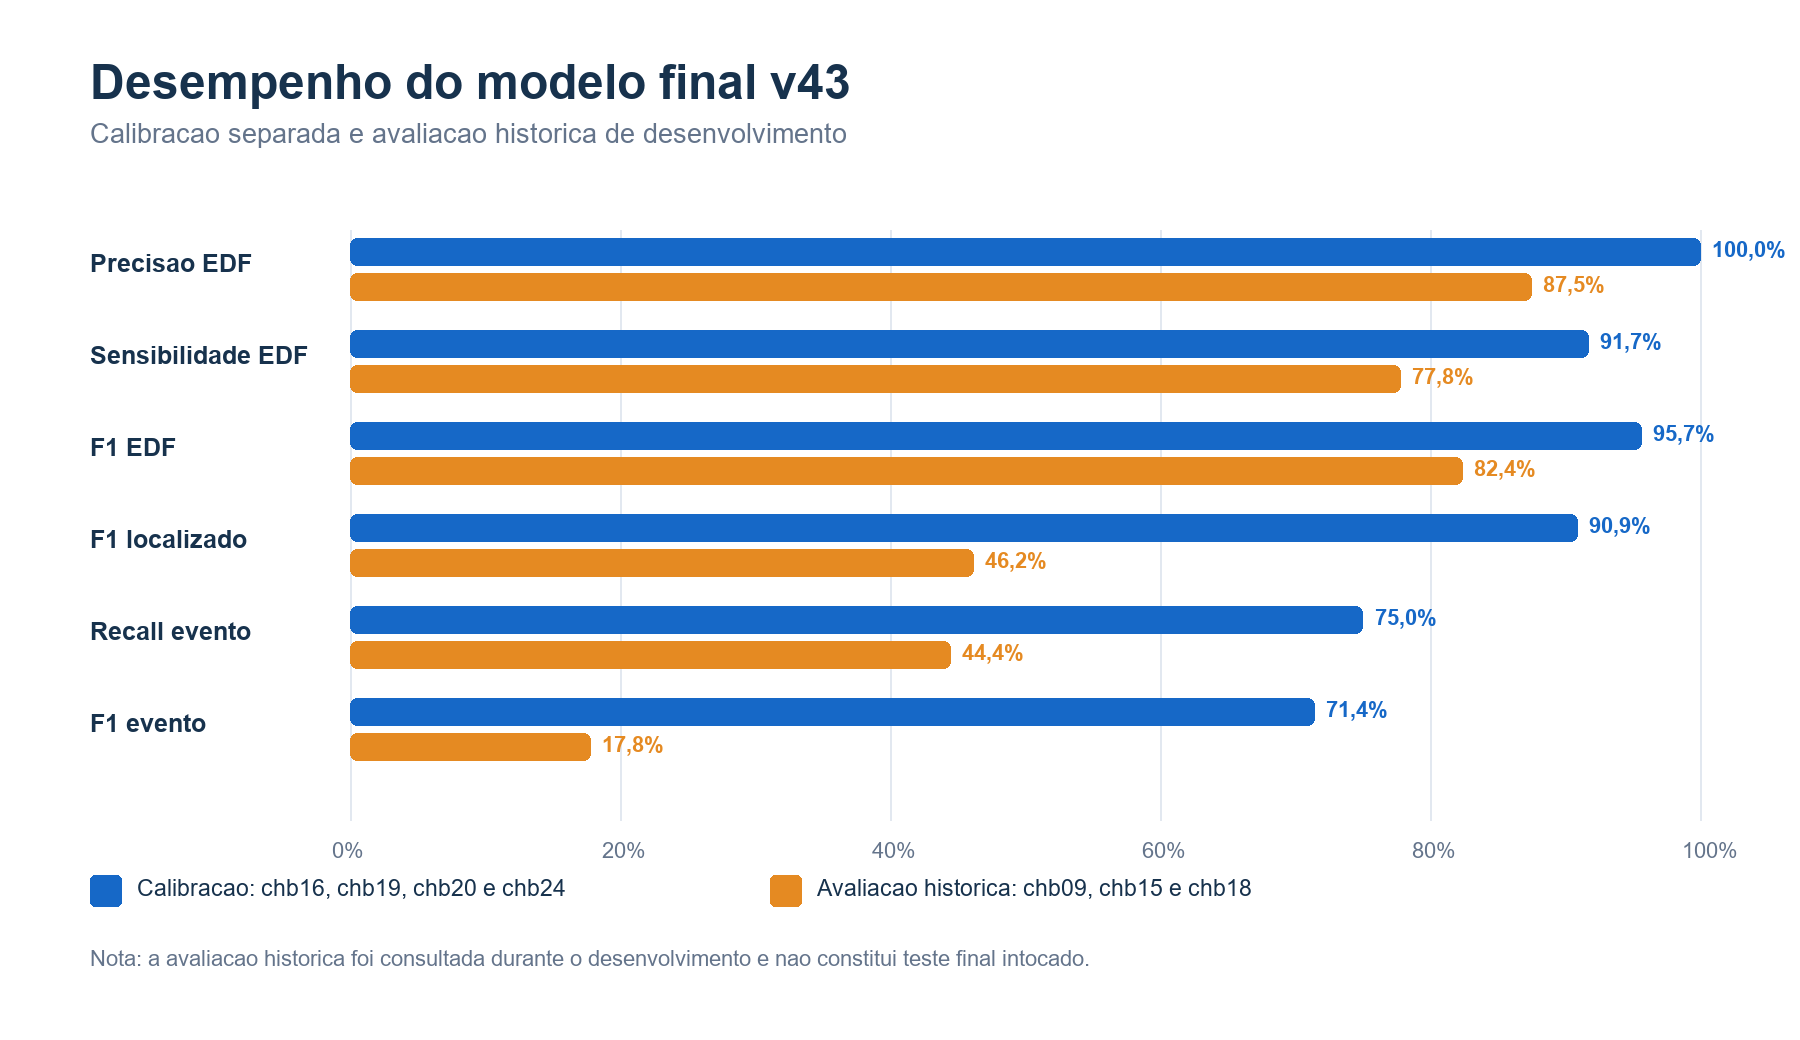
\includegraphics[width=13.60cm,height=0.72\textheight,keepaspectratio]{images/figura_17.png}\par
{\fontsize{10}{12}\selectfont Fonte: Elaborado pelo autor (2026).\par}
\end{figure}
Na calibração, a v43 atingiu F1 por EDF de 95,7\%, F1 localizado de 90,9\% e detectou 15 de 20 eventos, com 0,55 falso alarme por hora. A avaliação histórica apresentou F1 por EDF de 82,4\%, F1 localizado de 46,2\% e detecção de 4 de 9 eventos, com 2,08 falsos alarmes por hora. Entre os quatro eventos históricos detectados, a IoU temporal média foi 73,7\%, o erro absoluto médio de início foi 3,0 s e o erro absoluto médio de término foi 23,5 s. Essas médias descrevem apenas os eventos encontrados e não compensam as cinco crises perdidas. A diferença entre os conjuntos indica perda de generalização entre pacientes e impede interpretar a calibração como estimativa de desempenho clínico externo.

\begin{figure}[htbp]
\centering
\caption{Matrizes de confusão por EDF da v43.}
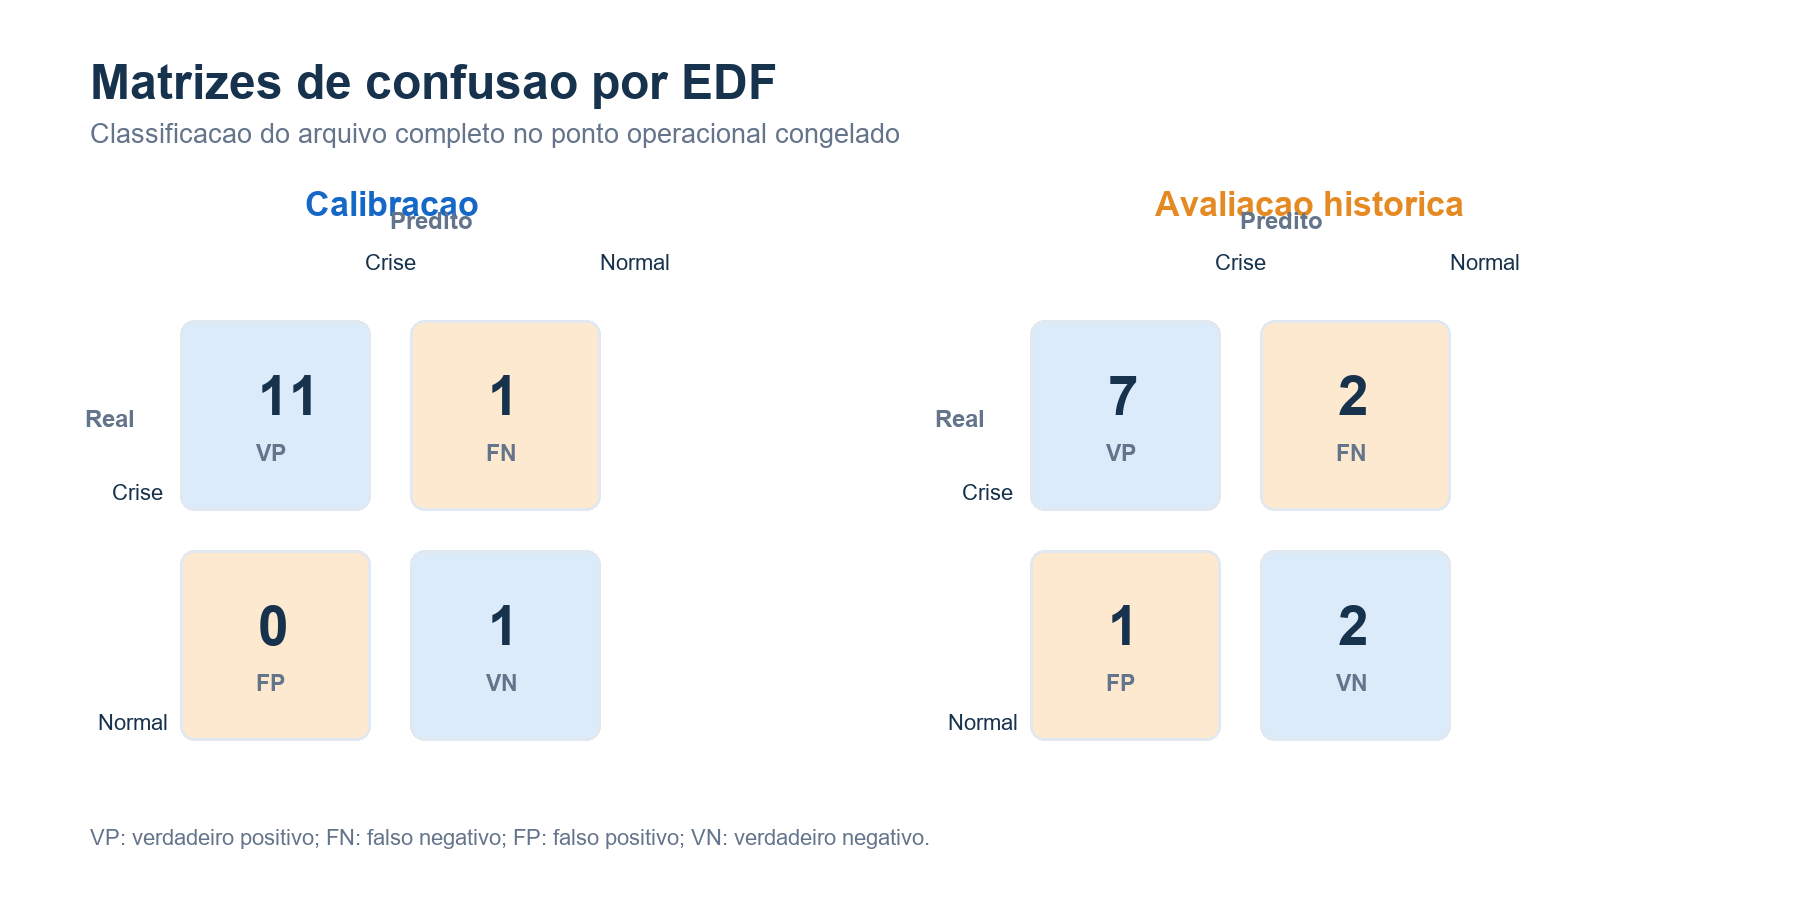
\includegraphics[width=13.60cm,height=0.72\textheight,keepaspectratio]{images/figura_20.png}\par
{\fontsize{10}{12}\selectfont Fonte: Elaborado pelo autor a partir dos artefatos v43 (2026).\par}
\end{figure}

\begin{figure}[htbp]
\centering
\caption{Eventos localizados e falsos alarmes por hora.}
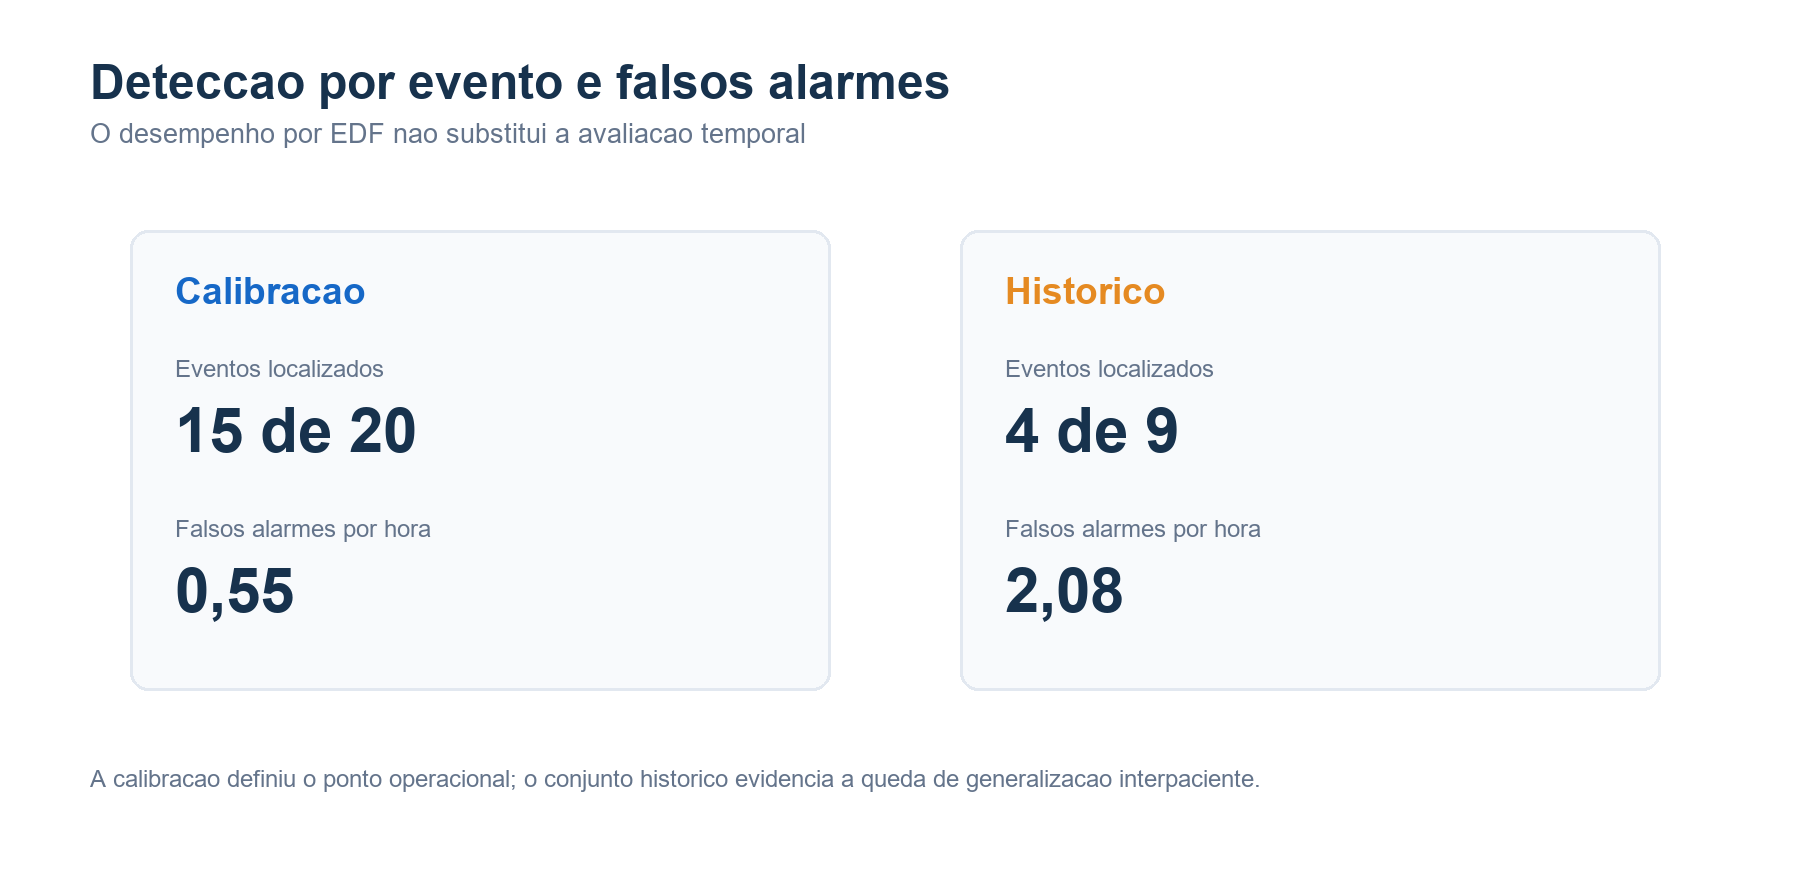
\includegraphics[width=13.60cm,height=0.72\textheight,keepaspectratio]{images/figura_18.png}\par
{\fontsize{10}{12}\selectfont Fonte: Elaborado pelo autor (2026).\par}
\end{figure}
O ponto operacional da v43 foi escolhido na curva de compromisso entre sensibilidade por evento e falsos alarmes por hora (FROC), com teto de 0,75 falso alarme por hora na calibração. Os valores apresentados no quadro representam esse ponto selecionado; não constituem uma curva FROC de teste externo. A precisão por EDF e a localização são analisadas separadamente, pois uma classificação correta do arquivo pode coexistir com uma crise perdida.

\Needspace{12\baselineskip}\section{Evolução experimental e estabilidade entre seeds}
A proposta registrada no TCC I previa a combinação das bases Bonn e CHB-MIT, validação k-fold e uso de Entropia de Shannon e Dinâmica Simbólica em uma CNN-LSTM. Um ensaio inicial de k-fold por janelas foi exploratório e não constitui a validação do modelo final. A avaliação passou a separar grupos antes do janelamento para examinar generalização interpaciente e evitar compartilhamento de janelas do mesmo grupo entre etapas. A base Bonn foi retirada da avaliação temporal final pelas diferenças de estrutura e anotação em relação aos EDFs contínuos da CHB-MIT.

A seleção das 15 características espectrais por canal decorreu das comparações de representação documentadas nos experimentos. A entropia espectral da v43 não equivale à feature histórica de Entropia de Shannon calculada diretamente do sinal, e a Dinâmica Simbólica não alimenta o modelo final. Também foi testada uma representação de sinal bruto, que não substituiu a escolhida. Essas alterações são decisões tomadas ao longo do desenvolvimento, não requisitos definidos dessa forma desde o início. Os resultados abaixo referem-se exclusivamente ao protocolo e aos artefatos da versão final.

A seleção da v43 não decorreu de uma única execução. Nas cinco seeds 42 a 46, a calibração apresentou média de 13,8 eventos detectados em 20, F1 por evento de 65,7\%, F1 localizado de 81,9\%, F1 por EDF de 96,4\% e 0,64 falso alarme por hora. A seed 42 alcançou 15/20 eventos, F1 localizado de 90,9\% e 0,55 falso alarme por hora. A variação entre seeds impede tratar esse melhor resultado isolado como desempenho esperado em novos pacientes.

Em comparação controlada com a CNN-BiLSTM anterior nas seeds 42 a 44, a fusão tardia da v43 elevou a média de eventos de 13,33 para 14,00 em 20, o F1 localizado de 75,0\% para 83,4\% e o F1 por EDF de 92,9\% para 97,1\%. Os falsos alarmes passaram de 0,58 para 0,63 por hora. Esses números são de calibração no mesmo protocolo e não demonstram generalização externa.

Experimentos posteriores avaliaram multirresolução, seleção de checkpoint e expansão dirigida dos dados. A v53, com 26 EDF no treino e três seeds, obteve média de 12,33/20 eventos, F1 localizado de 77,9\%, F1 por EDF de 92,5\% e 0,602 falso alarme por hora. Embora algumas crises tenham melhorado, o conjunto não superou a referência v43 no mesmo protocolo. Por isso, a v53 não substituiu o modelo integrado à aplicação.

A mineração de negativos difíceis foi examinada nas versões v55 e v56, usando somente pacientes de treino. A configuração forte v55 reduziu a média para 12,67/20 eventos e F1 localizado de 71,3\%, sem redução relevante dos falsos alarmes. A configuração leve v56 manteve 15/20 eventos na seed 42, mas reduziu o F1 localizado de 90,9\% para 85,7\%, com os mesmos 0,55 falso alarme por hora. Ambas foram rejeitadas para implantação.

\Needspace{12\baselineskip}\section{Análise dos erros e generalização}
A avaliação histórica em chb09, chb15 e chb18 localizou 4 de 9 eventos, com F1 localizado de 46,2\% e 2,08 falsos alarmes por hora. Esses pacientes haviam sido consultados durante o desenvolvimento e, portanto, os resultados descrevem a dificuldade interpaciente observada, sem constituir teste externo intocado. Crises não localizadas podem refletir baixa evidência ictal, fragmentação temporal ou escolha de candidato principal incorreto. A interpretação por evento é necessária porque F1 por EDF não identifica qual desses erros ocorreu.

Dois casos do artefato histórico ilustram essa distinção. Em \texttt{chb09\_19.edf}, o intervalo de referência reconstruído foi 5.298--5.362 s, enquanto o candidato correspondente foi 5.300--5.354 s. Houve 54 s de interseção, IoU de 84,4\%, início 2 s posterior e término 8 s anterior à referência. Em \texttt{chb15\_10.edf}, o evento de referência ocupou 1.080--1.114 s e nenhum candidato atingiu o critério de detecção. A ausência de candidato correspondente não permite, isoladamente, concluir se a causa foi um escore baixo ou o descarte pelo pós-processamento. Esses exemplos foram selecionados para ilustrar um acerto e uma falha já contabilizados, sem constituir novos experimentos.

Uma classificação positiva por EDF responde apenas se o arquivo recebeu um alerta válido. Ela não demonstra que todas as crises foram encontradas. No conjunto histórico, sete dos nove EDFs ictais receberam classificação positiva, mas somente quatro dos nove eventos corresponderam a candidatos válidos e apenas três EDFs ictais tiveram o candidato principal corretamente localizado. Por isso, o F1 por EDF de 82,4\%, o recall por evento de 44,4\% e o F1 localizado de 46,2\% descrevem aspectos distintos do mesmo resultado.

\Needspace{12\baselineskip}\section{Verificação do software e dos artefatos}
A integração foi verificada no fluxo local completo: autenticação, cadastro do paciente, leitura de EDF, visualização multicanal, recuperação de exame analisado, apresentação do escore, intervalo suspeito, sobreposição SHAP e emissão de laudo. O frontend foi compilado com TypeScript e Vite. Na rodada final direcionada aos componentes alterados, 46 testes do backend foram aprovados, abrangendo inferência sequencial, integração do SHAP, extração dos sinais para visualização, rotas de exames e persistência do pipeline. Essa seleção não equivale à execução integral de todos os testes do repositório. A integração real do Gradient SHAP com a saída temporal da v43 também foi verificada com entrada sintética compatível com o modelo, produzindo a imagem e a matriz de sobreposição; essa verificação comprova compatibilidade técnica, não desempenho em novo EDF. Na configuração final, a API iniciou com PostgreSQL e recuperou os registros migrados de usuários, pacientes, exames e predições. A comparação campo a campo com a origem confirmou a integridade dos registros.

Em 20 de outubro de 2026, a avaliação histórica foi reexecutada com os artefatos congelados da v43, seed 42, sem ajuste de parâmetros. Os códigos SHA-256 do modelo, do escalonador, dos metadados e da calibração coincidiram com o manifesto de artefatos. Com limiar 0,60, duração mínima de 18 s e fechamento de lacunas de 8 s, a execução reproduziu F1 por EDF de 82,4\%, F1 localizado de 46,2\%, detecção de 4 em 9 eventos e 2,08 falsos alarmes por hora. Essa reprodução confirma a consistência computacional dos resultados históricos registrados, mas não transforma o conjunto em teste externo intocado.

\begin{figure}[htbp]
\centering
\caption{Verificação de integridade dos artefatos da v43.}
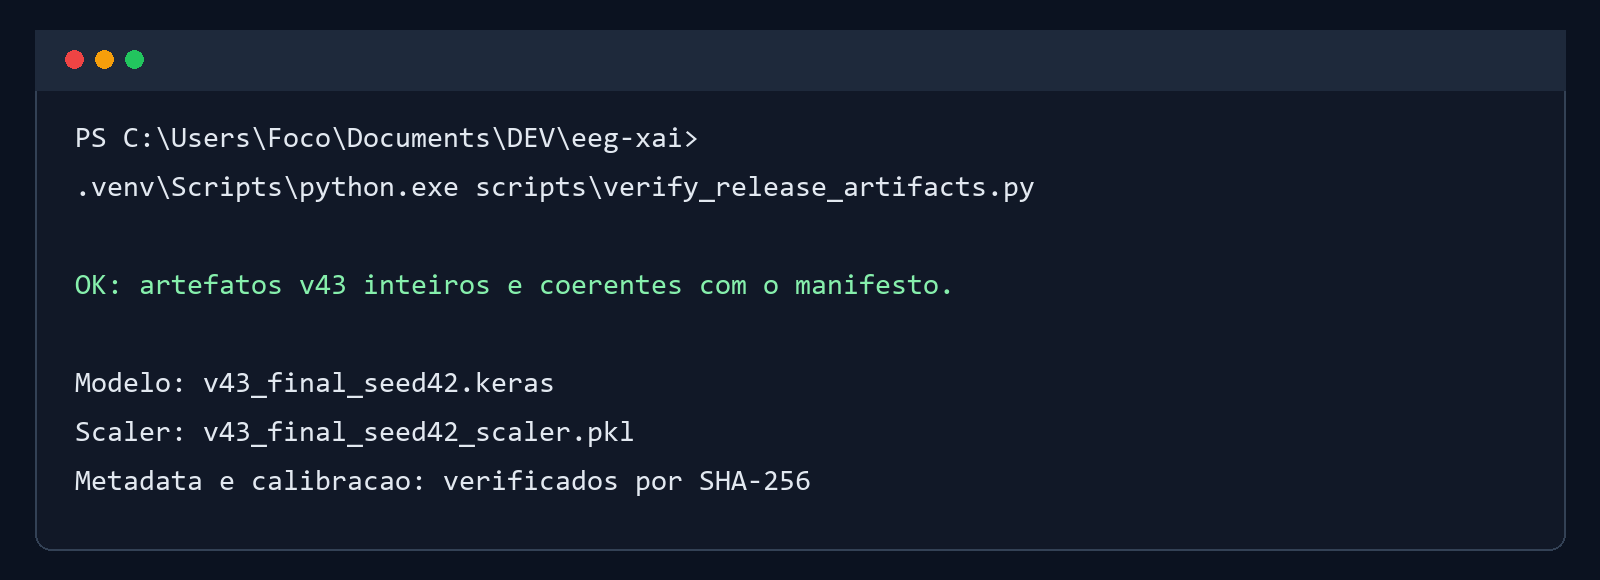
\includegraphics[width=13.60cm,height=0.72\textheight,keepaspectratio]{images/figura_19.png}\par
{\fontsize{10}{12}\selectfont Fonte: Elaborado pelo autor (2026).\par}
\end{figure}
\chapter{DISCUSSÃO}
Os resultados demonstram que o protótipo executa a proposta de apoio à análise temporal de EEG e apresenta evidências interpretáveis no mesmo contexto visual do sinal. A avaliação por EDF, isoladamente, mostrou-se insuficiente: mesmo quando o arquivo foi classificado corretamente, o sistema pôde deixar de localizar eventos específicos ou produzir alarmes fora do intervalo ictal. Por esse motivo, o estudo passou a registrar métricas por evento, localização temporal e falsos alarmes por hora.

A fusão tardia preservou a identidade dos canais por mais etapas da rede e foi superior às tentativas que agregavam precocemente a dimensão espacial. Entretanto, crises com morfologia, duração ou topografia pouco representadas no treino continuaram recebendo escores baixos. O pós-processamento temporal melhorou continuidade e reduziu fragmentação, mas não recuperou eventos que o primeiro estágio não representou.

O SHAP aumenta a inspecionabilidade ao destacar quais canais e janelas de características contribuíram para a sequência de pico. Essa explicação não comprova causalidade fisiológica, não substitui a interpretação do traçado e pode refletir correlações aprendidas pelo modelo. Sua utilidade deverá ser avaliada com especialistas em estudo posterior.

\Needspace{12\baselineskip}\section{Limitações e ameaças à validade}
\begin{itemize}[leftmargin=1.25cm,itemsep=0pt,topsep=0pt]
\item não existe conjunto CHB-MIT local completamente intocado, pois todos os grupos disponíveis foram utilizados em treino, calibração ou desenvolvimento histórico;
\item a calibração contém apenas quatro grupos de pacientes e vinte eventos, quantidade insuficiente para estimar generalização clínica;
\item não foi realizada validação externa em outra instituição ou base temporal multicanal equivalente;
\item não houve estudo formal de usabilidade com neurologistas ou técnicos de EEG;
\item o sistema é um protótipo local, sem validação de desempenho concorrente, conformidade integral com a LGPD ou regularização sanitária;
\item a rodada final de testes foi direcionada aos componentes modificados e não substitui uma execução integral da suíte em ambiente de integração.
\end{itemize}
\chapter{CONCLUSÃO}
Este trabalho desenvolveu um protótipo web de apoio à análise de EEG que integra autenticação, gestão de pacientes, ingestão de EDF, visualização multicanal, detecção temporal com CNN-BiLSTM, explicabilidade por Gradient SHAP e emissão de laudo. A implementação atende ao objetivo de reunir o fluxo técnico em uma única aplicação e mantém explícito que a saída da IA representa apoio à decisão, não diagnóstico autônomo.

A v43 apresentou desempenho elevado na calibração, mas a queda observada na avaliação histórica confirmou que a generalização interpaciente permanece o principal gargalo. Portanto, o protótipo pode ser apresentado como resultado de Engenharia de Software e experimento de IA explicável, mas não como sistema clinicamente validado.

Como trabalhos futuros, recomenda-se obter uma coorte externa mantida intocada, ampliar a diversidade de eventos ictais, avaliar arquiteturas espaciais e temporais em ablações controladas, calibrar o ponto operacional sem acesso ao teste, medir usabilidade com profissionais, completar controles de segurança e privacidade e avaliar requisitos regulatórios antes de qualquer uso assistencial.

\postextual\begin{SingleSpace}\chapter*{REFERÊNCIAS}\addcontentsline{toc}{chapter}{REFERÊNCIAS}
{\raggedright\setlength{\parindent}{0pt} ABOALAYON, K. A. I. et al. Seizure detection using EEG signals: a review of different EEG recording modalities, signal analysis techniques, and seizure detection systems. Informatics in Medicine Unlocked, v. 6, p. 1-18, 2016. Disponível em: \url{https://catalog.nlm.nih.gov/discovery/fulldisplay?docid=alma9916189513406676&context=L&vid=01NLM_INST:01NLM_INST&lang=en.} Acesso em: 05 nov. 2025.\par}\smallskip

{\raggedright\setlength{\parindent}{0pt} ACETO, G.; PERSICO, V.; PESCO, A. Industry 4.0 and Health: Internet of Things, Big Data, and Cloud Computing for Healthcare 4.0. Journal of Industrial Information Integration, v. 18, p. 100129, 2020. Disponível em: \url{https://www.sciencedirect.com/science/article/abs/pii/S2452414X19300135} . Acesso em: 05 nov. 2025.\par}\smallskip

{\raggedright\setlength{\parindent}{0pt} ACHARYA, U. R. et al. Deep convolutional neural network for the automated detection and diagnosis of seizure using EEG signals. Computers in Biology and Medicine, v. 100, p. 270-278, 2018. Disponível em: \url{https://www.sciencedirect.com/science/article/abs/pii/S0010482517303153} . Acesso em: 06 nov. 2025.\par}\smallskip

{\raggedright\setlength{\parindent}{0pt} ADADI, A.; BERRADA, M. Peeking inside the black-box: a survey on explainable artificial intelligence (XAI). IEEE Access, v. 6, p. 52138-52160, 2018. Disponível em: \url{https://www.researchgate.net/publication/327709435_Peeking_Inside_the_Black-Box_A_Survey_on_Explainable_Artificial_Intelligence_XAI.} Acesso em: 06 nov. 2025.\par}\smallskip

{\raggedright\setlength{\parindent}{0pt} AGARWAL, R. et al. The digital transformation of healthcare: current status and the road ahead. Information Systems Research, v. 21, n. 4, p. 796-809, 2010. Disponível em: \url{https://www.researchgate.net/publication/220079558_The_Digital_Transformation_of_Healthcare_Current_Status_and_the_Road_Ahead} . Acesso em: 07 nov. 2025.\par}\smallskip

{\raggedright\setlength{\parindent}{0pt} AMANN, J. et al. Explainability for artificial intelligence in healthcare: a multidisciplinary perspective. BMC Medical Informatics and Decision Making, v. 20, n. 1, p. 310, 2020. Disponível em: \url{https://www.researchgate.net/publication/346542270_Explainability_for_artificial_intelligence_in_healthcare_a_multidisciplinary_perspective} . Acesso em: 07 nov. 2025.\par}\smallskip

{\raggedright\setlength{\parindent}{0pt} ARRIETA, A. B. et al. Explainable Artificial Intelligence (XAI): Concepts, taxonomies, opportunities and challenges toward responsible AI. Information Fusion, v. 58, p. 82-115, 2020. Disponível em: \url{https://www.sciencedirect.com/science/article/abs/pii/S1566253519308103.} Acesso em: 08 nov. 2025.\par}\smallskip

{\raggedright\setlength{\parindent}{0pt} BANKS, A.; PORCELLO, E. Learning React: Modern Patterns for Developing React Apps. 2. ed. Sebastopol: O'Reilly Media, 2020. Disponível em: \url{https://phanindra-reddy.github.io/portfolio/static/media/learningreact.da253db3.pdf}\par}\smallskip

{\raggedright\setlength{\parindent}{0pt} BECK, K. et al. Manifesto for Agile Software Development. 2001. Disponível em: \url{http://agilemanifesto.org/.} Acesso em: 16 nov. 2025.\par}\smallskip

{\raggedright\setlength{\parindent}{0pt} BRASIL. Agência Nacional de Vigilância Sanitária. Resolução da Diretoria Colegiada - RDC nº 657, de 24 de março de 2022. Dispõe sobre a regularização de software como dispositivo médico. Brasília, DF: Anvisa, 2022. Disponível em: \url{https://www.gov.br/anvisa/.} Acesso em: 13 out. 2026.\par}\smallskip

{\raggedright\setlength{\parindent}{0pt} BRASIL. Agência Nacional de Vigilância Sanitária. Software como dispositivo médico: perguntas e respostas. Brasília, DF: Anvisa, 2022. Disponível em: \url{https://www.gov.br/anvisa/pt-br/centraisdeconteudo/publicacoes/produtos-para-a-saude/manuais/software-como-dispositivo-medico-perguntas-e-respostas.} Acesso em: 13 out. 2026.\par}\smallskip

{\raggedright\setlength{\parindent}{0pt} BRASIL. Governo Digital. Modelo de Acessibilidade em Governo Eletrônico - eMAG, versão 3.1. Brasília, DF: Governo Federal. Disponível em: \url{https://www.gov.br/governodigitallogin/pt-br/acessibilidade-e-usuario/acessibilidade-digital/modelo-de-acessibilidade.} Acesso em: 13 out. 2026.\par}\smallskip

{\raggedright\setlength{\parindent}{0pt} CRAIK, A.; HE, Y.; CONTRERAS-VIDAL, J. L. Deep learning for electroencephalogram (EEG) classification tasks: a review. Journal of Neural Engineering, v. 16, n. 3, 2019. Disponível em: \url{https://pubmed.ncbi.nlm.nih.gov/30808014/} . Acesso em: 08 nov. 2025.\par}\smallskip

{\raggedright\setlength{\parindent}{0pt} ELMASRI, R.; NAVATHE, S. B. Fundamentals of Database Systems. 6. ed. Boston: Addison-Wesley, 2011. Disponível em: \url{https://www.uoitc.edu.iq/images/documents/informatics-institute/Competitive_exam/Database_Systems.pdf}\par}\smallskip

{\raggedright\setlength{\parindent}{0pt} ESTEVA, A. et al. A guide to deep learning in healthcare. Nature Medicine, v. 25, n. 1, p. 24-29, 2019. Disponível em: \url{https://pubmed.ncbi.nlm.nih.gov/30617335/.} Acesso em: 09 nov. 2025.\par}\smallskip

{\raggedright\setlength{\parindent}{0pt} FAUST, O. et al. Deep learning for healthcare applications based on physiological signals: A review. Computer Methods and Programs in Biomedicine, v. 161, p. 1-13, 2018. Disponível em: \url{https://www.sciencedirect.com/science/article/abs/pii/S0169260718301226} . Acesso em: 09 nov. 2025.\par}\smallskip

{\raggedright\setlength{\parindent}{0pt} FIELDING, R. T. Architectural Styles and the Design of Network-based Software Architectures. 2000. Tese (Doutorado em Ciência da Computação) - University of California, Irvine, 2000. Disponível em: \url{https://roy.gbiv.com/pubs/dissertation/fielding_dissertation.pdf}\par}\smallskip

{\raggedright\setlength{\parindent}{0pt} FOWLER, M. Refactoring: Improving the Design of Existing Code. 2. ed. Boston: Addison-Wesley, 2018. Disponível em: \url{https://www.kufunda.net/publicdocs/Refatora%C3%A7%C3%A3o%20(Fowler,%20Martin).pdf}\par}\smallskip

{\raggedright\setlength{\parindent}{0pt} GOLDBERGER, A. L. et al. PhysioBank, PhysioToolkit, and PhysioNet: components of a new research resource for complex physiologic signals. Circulation, v. 101, n. 23, p. e215-e220, 2000. Disponível em: \url{https://www.ahajournals.org/doi/10.1161/01.cir.101.23.e215} . Acesso em: 10 nov. 2025.\par}\smallskip

{\raggedright\setlength{\parindent}{0pt} GRAMFORT, A. et al. MEG and EEG data analysis with MNE-Python. Frontiers in Neuroscience, v. 7, p. 267, 2013. Disponível em: \url{https://www.frontiersin.org/journals/neuroscience/articles/10.3389/fnins.2013.00267/full.} Acesso em: 10 nov. 2025.\par}\smallskip

{\raggedright\setlength{\parindent}{0pt} GUNNING, D. et al. XAI—Explainable artificial intelligence. Science Robotics, v. 4, n. 37, 2019. Disponível em: \url{https://www.researchgate.net/publication/338039379_XAI-Explainable_artificial_intelligence} . Acesso em: 11 nov. 2025.\par}\smallskip

{\raggedright\setlength{\parindent}{0pt} HOCHREITER, S.; SCHMIDHUBER, J. Long short-term memory. Neural Computation, v. 9, n. 8, p. 1735-1780, 1997. Disponível em: \url{https://www.researchgate.net/publication/13853244_Long_Short-Term_Memory.} Acesso em: 11 nov. 2025.\par}\smallskip

{\raggedright\setlength{\parindent}{0pt} KLEPPMANN, M. Designing Data-Intensive Applications. Sebastopol: O'Reilly Media, 2017. Disponível em: \url{https://www.oreilly.com/library/view/designing-data-intensive-applications/9781491903063/}\par}\smallskip

{\raggedright\setlength{\parindent}{0pt} LECUN, Y.; BENGIO, Y.; HINTON, G. Deep learning. Nature, v. 521, p. 436-444, 2015. Disponível em: \url{https://www.nature.com/articles/nature14539.} Acesso em: 12 nov. 2025.\par}\smallskip

{\raggedright\setlength{\parindent}{0pt} LUNDBERG, S. M.; LEE, S.-I. A unified approach to interpreting model predictions. In: ADVANCES IN NEURAL INFORMATION PROCESSING SYSTEMS, 30. Anais... Long Beach, CA: NeurIPS, 2017. Disponível em: \url{https://papers.nips.cc/paper_files/paper/2017/hash/8a20a8621978632d76c43dfd28b67767-Abstract.html} . Acesso em: 12 nov. 2025.\par}\smallskip

{\raggedright\setlength{\parindent}{0pt} MCKINNEY, W. Python for Data Analysis. Sebastopol: O'Reilly Media, 2012.\par}\smallskip

{\raggedright\setlength{\parindent}{0pt} META PLATFORMS. React: the library for web and native user interfaces. Disponível em: \url{https://react.dev/.} Acesso em: 13 out. 2026.\par}\smallskip

{\raggedright\setlength{\parindent}{0pt} MOREIRA, Karollyne Evangelista; MARQUES, Eduardo Henrique Guimarães; TORQUATO, Thiane Marques; SOUZA, Lynwood Livi de. Identificação de Padrões Genéticos para Diagnóstico de Doenças Utilizando Inteligência Artificial (Relatório Final de Iniciação em Desenvolvimento Tecnológico e Inovação - PIBITI). Uruaçu: Instituto Federal de Educação, Ciência e Tecnologia de Goiás (IFG), 2025.\par}\smallskip

{\raggedright\setlength{\parindent}{0pt} NEWMAN, S. Building Microservices: Designing Fine-Grained Systems. 2. ed. Sebastopol: O'Reilly Media, 2021. Disponível em: \url{https://github.com/iamindian/References_Books/blob/master/Building%20Microservices%20Designing%20Fine-Grained%20Systems%202nd%20By%20Sam%20Newman.pdf}\par}\smallskip

{\raggedright\setlength{\parindent}{0pt} NIEDERMEYER, E.; LOPES DA SILVA, F. H. Electroencephalography: Basic Principles, Clinical Applications, and Related Fields. 5. ed. Philadelphia: Lippincott Williams \& Wilkins, 2005. Disponível em: \url{https://books.google.com.br/books/about/Electroencephalography.html?id=tndqYGPHQdEC&redir_esc=y}\par}\smallskip

{\raggedright\setlength{\parindent}{0pt} PRESSMAN, R. S.; MAXIM, B. R. Engenharia de Software: Uma Abordagem Profissional. 8. ed. Porto Alegre: AMGH, 2016.\par}\smallskip

{\raggedright\setlength{\parindent}{0pt} RAGHUPATHI, W.; RAGHUPATHI, V. Big data analytics in healthcare: promise and potential. Health Information Science and Systems, v. 2, n. 3, 2014. Disponível em: \url{https://pubmed.ncbi.nlm.nih.gov/25825667/} . Acesso em: 13 nov. 2025.\par}\smallskip

{\raggedright\setlength{\parindent}{0pt} RAMÍREZ, S. FastAPI. Disponível em: \url{https://fastapi.tiangolo.com/.} Acesso em: 18 nov. 2025.\par}\smallskip

{\raggedright\setlength{\parindent}{0pt} REISMAN, M. EHRs: the challenge of making electronic data usable and interoperable. Pharmacy and Therapeutics, v. 42, n. 9, p. 572-575, 2017. Disponível em: \url{https://pmc.ncbi.nlm.nih.gov/articles/PMC5565131/.} Acesso em: 13 out. 2026.\par}\smallskip

{\raggedright\setlength{\parindent}{0pt} RICHARDS, M. Software Architecture Patterns. Sebastopol: O'Reilly Media, 2015.\par}\smallskip

{\raggedright\setlength{\parindent}{0pt} ROY, Y. et al. Deep learning-based electroencephalography analysis: a comprehensive review. Journal of Neural Engineering, v. 16, n. 5, 2019. Disponível em: \url{https://iopscience.iop.org/article/10.1088/1741-2552/ab260c} . Acesso em: 14 nov. 2025.\par}\smallskip

{\raggedright\setlength{\parindent}{0pt} SHANNON, C. E. A mathematical theory of communication. The Bell System Technical Journal, v. 27, n. 3, p. 379–423, 1948. Disponível em: \url{https://people.math.harvard.edu/~ctm/home/text/others/shannon/entropy/entropy.pdf} . Acesso em: 14 nov. 2025.\par}\smallskip

{\raggedright\setlength{\parindent}{0pt} SHOEB, A. H. Application of machine learning to epileptic seizure onset detection and treatment. 2009. Tese (Doutorado) - Massachusetts Institute of Technology, Cambridge, 2009.\par}\smallskip

{\raggedright\setlength{\parindent}{0pt} SOMMERVILLE, I. Software Engineering. 9. ed. Boston: Addison-Wesley, 2011.\par}\smallskip

{\raggedright\setlength{\parindent}{0pt} SUTTON, R. T. et al. An overview of clinical decision support systems: benefits, risks, and strategies for success. NPJ Digital Medicine, v. 3, n. 17, 2020. Disponível em: \url{https://www.nature.com/articles/s41746-020-0221-y} . Acesso em: 15 nov. 2025.\par}\smallskip

{\raggedright\setlength{\parindent}{0pt} TATUM, W. O. Handbook of EEG Interpretation. 2. ed. New York: Demos Medical Publishing, 2014. Disponível em: \url{https://books.google.com/books?id=PZnSCgAAQBAJ.} Acesso em: 15 out. 2026.\par}\smallskip

{\raggedright\setlength{\parindent}{0pt} TOPOL, E. J. High-performance medicine: the convergence of human and artificial intelligence. Nature Medicine, v. 25, p. 44-56, 2019. Disponível em: \url{https://pubmed.ncbi.nlm.nih.gov/30617339/} . Acesso em: 15 nov. 2025.\par}\smallskip

{\raggedright\setlength{\parindent}{0pt} VAN ROSSUM, G.; DRAKE, F. L. Python 3 Reference Manual. Scotts Valley, CA: CreateSpace, 2009.\par}\smallskip

{\raggedright\setlength{\parindent}{0pt} WHO - WORLD HEALTH ORGANIZATION. Epilepsy. 2024. Disponível em: \url{https://www.who.int/news-room/fact-sheets/detail/epilepsy.} Acesso em: 17 nov. 2025.\par}\smallskip

{\raggedright\setlength{\parindent}{0pt} YAMASHITA, R. et al. Convolutional neural networks: an overview and application in radiology. Insights into Imaging, v. 9, n. 4, p. 611-629, 2018. Disponível em: \url{https://pubmed.ncbi.nlm.nih.gov/29934920/.} Acesso em: 16 nov. 2025.\par}\smallskip

\end{SingleSpace}\begin{apendicesenv}\chapter{RECURSOS E CRONOGRAMA}
O desenvolvimento foi organizado conforme o cronograma do Quadro 10. Os recursos previstos são apresentados no Quadro 9, cujo total é R\$ 3.650,00.

\Needspace{12\baselineskip}\section{Recursos}
\FloatBarrier\Needspace{9\baselineskip}
\captionof{table}{Descrição Orçamentária}\nopagebreak[4]
\begingroup
\fontsize{9}{11}\selectfont
\setlength{\tabcolsep}{2pt}
\renewcommand{\arraystretch}{1.15}
\addtocounter{table}{-1}
\begin{longtable}{|>{\raggedright\arraybackslash}p{0.050\textwidth}|>{\raggedright\arraybackslash}p{0.250\textwidth}|>{\raggedright\arraybackslash}p{0.080\textwidth}|>{\raggedright\arraybackslash}p{0.200\textwidth}|>{\raggedright\arraybackslash}p{0.150\textwidth}|>{\raggedright\arraybackslash}p{0.160\textwidth}|}
\hline
\textbf{Nº} & \textbf{Descrição} & \textbf{Quant.} & \textbf{Fonte financiadora} & \textbf{Valor Unitário} & \textbf{Valor Total} \\ \hline
\endfirsthead
\hline
\textbf{Nº} & \textbf{Descrição} & \textbf{Quant.} & \textbf{Fonte financiadora} & \textbf{Valor Unitário} & \textbf{Valor Total} \\ \hline
\endhead
1 & PC Desktop (i3, 16GB RAM, SSD) & 1 & Recurso próprio & R\$ 3.500,00 & R\$ 3.500,00 \\ \hline
2 & Ferramentas de API & 1 & Recurso próprio & R\$ 50,00 & R\$ 50,00 \\ \hline
3 & Domínio Web e Hospedagem & 1 ano & Recurso próprio & R\$ 100,00 & R\$ 100,00 \\ \hline
\multicolumn{6}{|r|}{\textbf{TOTAL: R\$ 3.650,00}} \\ \hline
\end{longtable}
\endgroup
\nopagebreak[4]{\centering\fontsize{10}{12}\selectfont Fonte: Elaborado pelo autor (2026).\par}
\Needspace{12\baselineskip}\section{Cronograma}
\FloatBarrier\Needspace{9\baselineskip}
\captionof{table}{Cronograma de trabalho dividido em meses e atividades a serem realizadas}\nopagebreak[4]
\begingroup
\scriptsize
\setlength{\tabcolsep}{2pt}
\renewcommand{\arraystretch}{1.15}
\addtocounter{table}{-1}
\begin{longtable}{|>{\raggedright\arraybackslash}p{0.200\textwidth}|>{\raggedright\arraybackslash}p{0.055\textwidth}|>{\raggedright\arraybackslash}p{0.055\textwidth}|>{\raggedright\arraybackslash}p{0.055\textwidth}|>{\raggedright\arraybackslash}p{0.055\textwidth}|>{\raggedright\arraybackslash}p{0.055\textwidth}|>{\raggedright\arraybackslash}p{0.055\textwidth}|>{\raggedright\arraybackslash}p{0.055\textwidth}|>{\raggedright\arraybackslash}p{0.055\textwidth}|>{\raggedright\arraybackslash}p{0.055\textwidth}|>{\raggedright\arraybackslash}p{0.055\textwidth}|>{\raggedright\arraybackslash}p{0.055\textwidth}|>{\raggedright\arraybackslash}p{0.055\textwidth}|}
\hline
\textbf{Atividades} & \multicolumn{12}{c|}{\textbf{2026}} \\ \hline
\endfirsthead
\hline
\textbf{Atividades} & \multicolumn{12}{c|}{\textbf{2026}} \\ \hline
\endhead
Atividades & Jan. & Fev. & Mar. & Abr. & Mai. & Jun. & Jul. & Ago. & Set. & Out. & Nov. & Dez. \\ \hline
Levantamento do referencial teórico & X & X & X &  &  &  &  &  &  &  &  &  \\ \hline
Levantamento dos requisitos &  & X & X &  &  &  &  &  &  &  &  &  \\ \hline
Desenvolvimento do sistema &  & X & X & X & X & X & X & X & X & X &  &  \\ \hline
Testes &  &  &  & X & X & X & X & X &  & X & X &  \\ \hline
Apresentação TCC 1 &  &  &  &  &  & X &  &  &  &  &  &  \\ \hline
Apresentação TCC 2 &  &  &  &  &  &  &  &  &  &  &  & X \\ \hline
\end{longtable}
\endgroup
\nopagebreak[4]{\centering\fontsize{10}{12}\selectfont Fonte: Elaborado pelo autor (2026).\par}
\end{apendicesenv}

\end{document}
